% ============================================================================
% 本科毕业设计 (论文) 答辩演示文稿
% 编译方式：xelatex -> bibtex -> xelatex -> xelatex
% ============================================================================

\documentclass{beamer}

% ---------- 导入配置文件 ----------
% ============================================================================
% 版式配置文件 (layout.tex)
% 包含：包导入、页面布局、列表样式、代码块设置等
% ============================================================================

% ---------- 基础宏包 ----------
\usepackage{ctex, hyperref}
\usepackage[T1]{fontenc}

% 数学与表格宏包
\usepackage{latexsym,amsmath,xcolor,multicol,booktabs,calligra}
\usepackage{graphicx,listings,stackengine}
\usepackage{caption, subfigure}
\usepackage{tikz}
\usetikzlibrary{positioning, arrows.meta, shapes.geometric}
\usepackage{algorithm, algorithmic}

% PSTricks (可选，用于绘制图形示例)
% 如果缺少 pstricks，请安装：texlive-pstricks 或 miktex-pstricks
\IfFileExists{pstricks.sty}{\usepackage{pstricks}}{}

% ---------- 厦门大学主题 ----------
% 主题颜色：厦大蓝（默认）
\xdefinecolor{xmu}{RGB}{30 , 55 , 113}

% ============================================================================
% 厦门大学 Beamer 主题配置
% ============================================================================

\mode<presentation>

% ---------- 主题颜色定义 ----------
% 默认：厦大蓝，无背景
\xdefinecolor{xmu}{RGB}{30 , 55 , 113}
\xdefinecolor{xmu@orange}{RGB}{240,140,0}

% ---------- 外部主题 ----------
\useoutertheme[footline=authorinstitutetitle,subsection=false]{smoothbars}

% ---------- 页脚模板 ----------
\makeatletter
\newcommand{\frameofframes}{/}
\newcommand{\setframeofframes}[1]{\renewcommand{\frameofframes}{#1}}

\defbeamertemplate*{footline}{xmu_beamer}{%
	\leavevmode%
	\hbox{%
		\begin{beamercolorbox}[wd=.25\paperwidth,ht=2.5ex,dp=1.125ex,center]{title in head/foot}%
			\usebeamerfont{author in head/foot}\insertshortauthor
		\end{beamercolorbox}%
		\begin{beamercolorbox}[wd=.25\paperwidth,ht=2.5ex,dp=1.125ex,center]{title in head/foot}%
			\usebeamerfont{author in head/foot}\insertshortdate
		\end{beamercolorbox}%
		\begin{beamercolorbox}[wd=.435\paperwidth,ht=2.5ex,dp=1.125ex,center]{author in head/foot}%
			\usebeamerfont{title in head/foot}\insertshorttitle
		\end{beamercolorbox}%
		\begin{beamercolorbox}[wd=0.065\paperwidth,ht=2.5ex,dp=1.125ex,right]{author in head/foot}%
			\insertframenumber{} / \inserttotalframenumber\hspace*{1ex}
	\end{beamercolorbox}}%
	\vskip0pt%
}
\makeatother

% ---------- 内部主题 ----------
\useinnertheme{circles}
\usefonttheme{professionalfonts}

% ---------- 颜色设置 ----------
\setbeamercolor{footline}{bg=xmu}
\setbeamercolor{frametitle}{bg=xmu,fg=white}
\setbeamercolor{title}{bg=xmu}
\setbeamertemplate{bibliography item}[text]
\setbeamertemplate{caption}[numbered]

% 引用颜色设置为红色
\setbeamercolor{bibliography entry}{fg=red}
\setbeamercolor{citation}{fg=red}

\setbeamercolor{palette primary}{use=structure,fg=white,bg=structure.fg}
\setbeamercolor{palette secondary}{use=structure,fg=white,bg=structure.fg!75!black}
\setbeamercolor{palette tertiary}{use=structure,fg=white,bg=structure.fg!50!black}
\setbeamercolor{palette quaternary}{fg=white,bg=structure.fg!50!black}
\setbeamercolor{titlelike}{parent=palette primary}

% Block 颜色
\setbeamercolor{block title}{bg=xmu,fg=white}
\setbeamercolor{block title alerted}{use=alerted text,fg=white,bg=xmu@orange}
\setbeamercolor{block title example}{use={normal text,example text},bg=white,fg=xmu}

% 其他颜色
\setbeamercolor{fine separation line}{}
\setbeamercolor{item projected}{fg=white}
\setbeamercolor{palette sidebar primary}{use=normal text,fg=normal text.fg}
\setbeamercolor{palette sidebar quaternary}{use=structure,fg=structure.fg}
\setbeamercolor{palette sidebar secondary}{use=structure,fg=structure.fg}
\setbeamercolor{palette sidebar tertiary}{use=normal text,fg=normal text.fg}
\setbeamercolor{section in sidebar}{fg=brown}
\setbeamercolor{section in sidebar shaded}{fg=grey}
\setbeamercolor{separation line}{}
\setbeamercolor{sidebar}{bg=xmu}
\setbeamercolor{sidebar}{parent=palette primary}
\setbeamercolor{structure}{fg=xmu}
\setbeamercolor{subsection in sidebar}{fg=brown}
\setbeamercolor{subsection in sidebar shaded}{fg=grey}

% ---------- 章节开始时显示目录 ----------
\AtBeginSection[]{
	\begin{frame}
		\tableofcontents[sectionstyle=show/shaded,subsectionstyle=show/shaded/hide,subsubsectionstyle=hide]
	\end{frame}
}


\mode<all>


% ---------- 列表环境设置 ----------
% 设置 itemize 的标记符号
\setbeamertemplate{itemize items}[circle]
\setbeamertemplate{itemize subitem}{--}

% ---------- 代码 listings 设置 ----------
\lstset{
    basicstyle=\ttfamily\small,
    keywordstyle=\bfseries\color{red!0!green!0!blue!100},
    emphstyle=\ttfamily\color{red!100!green!0!blue!0},
    stringstyle=\color{red!0!green!100!blue!0},
    numbers=left,
    numberstyle=\small\color{gray!50},
    rulesepcolor=\color{red!20!green!20!blue!20},
    frame=shadowbox,
    breaklines=true,
    breakatwhitespace=true,
}

% ---------- 图片路径设置 ----------
\graphicspath{{pic/}{../pic/}}

% ---------- 超链接设置 ----------
\hypersetup{
    colorlinks=true,
    linkcolor=xmu,
    filecolor=magenta,
    urlcolor=xmu,
    citecolor=red!70!white,
}
    % 版式配置：宏包、主题、样式设置
% ============================================================================
% 宏定义文件 (macros.tex)
% 包含：自定义命令、文档元数据等
% ============================================================================

% ---------- 文档元数据 ----------
\author[邓凯璇]{邓凯璇}
\title{基于表格型 Q-Learning 的运动想象时间窗优化方法}
\subtitle{本科毕业设计 (论文) 答辩}
\institute{厦门大学 信息学院}
\date{\today}

% ---------- 自定义命令 ----------
% 用于显示 LaTeX 命令（红色）
\def\cmd#1{\texttt{\color{red}\footnotesize $\backslash$#1}}

% 用于显示 LaTeX 环境（蓝色）
\def\env#1{\texttt{\color{blue}\footnotesize #1}}
    % 宏定义：自定义命令、文档元数据

% ---------- 参考文献设置 (必须在 document 之前) ----------
\bibliographystyle{plain}

% ============================================================================
% 文档正文
% ============================================================================

\begin{document}

% ---------- 标题页 ----------
\begin{frame}
    \titlepage
    \begin{figure}[htpb]
        \begin{center}
            \includegraphics[width=0.2\linewidth]{xmu-logo.pdf}
        \end{center}
    \end{figure}
\end{frame}

% ---------- 目录页 ----------
\begin{frame}
    \tableofcontents[sectionstyle=show,subsectionstyle=show/shaded/hide]
\end{frame}

% ---------- 各章节内容 ----------
% ============================================================================
% 第一章：研究背景与意义
% ============================================================================

\section{研究背景}

\begin{frame}{研究背景}
    \begin{block}{运动想象脑机接口 (MI-BCI)}
        \begin{itemize}
            \item 通过解码运动想象诱发的 ERD 现象实现用户意图识别
            \item 为运动功能障碍患者提供重建运动功能的可能性
            \item 无需外部刺激、用户可自主控制
        \end{itemize}
    \end{block}
    
    \vspace{0.5cm}
    \begin{alertblock}{关键问题：时间窗选择}
        \begin{itemize}
            \item ERD 动态特性存在显著的\textbf{个体间差异}
            \item 时间窗长度需在\textbf{信息完整性}与\textbf{噪声抑制}之间平衡
            \item 在线 BCI 系统需要\textbf{毫秒级响应}
        \end{itemize}
    \end{alertblock}
\end{frame}

\begin{frame}{时间窗选择的重要性}
    \begin{center}
    \begin{tabular}{|c|c|c|}
        \hline
        \textbf{因素} & \textbf{影响} & \textbf{挑战} \\
        \hline
        个体差异 & ERD 模式不同 & 固定窗口无法适应 \\
        \hline
        信噪比 & 窗口长度影响 & 需要权衡 \\
        \hline
        实时性 & 响应延迟 & 在线决策要求 \\
        \hline
    \end{tabular}
    \end{center}
    
    \vspace{0.5cm}
    \begin{exampleblock}{结论}
        自适应时间窗优化是提升 MI-BCI 分类性能的关键途径
    \end{exampleblock}
\end{frame}

% ============================================================================
% 问题提出
% ============================================================================
\section{问题提出}

\begin{frame}{现有方法及其局限}
    \begin{table}[h]
        \centering
        \footnotesize
        \begin{tabular}{l|c|c|c}
            \hline
            \textbf{方法} & \textbf{计算开销} & \textbf{适应性} & \textbf{可解释性} \\
            \hline
            固定时间窗 & 低 & 差 & 好 \\
            滑动窗 & 中 & 中 & 中 \\
            贝叶斯优化 & 高 & 中 & 中 \\
            深度强化学习 & 很高 & 好 & 差 \\
            \hline
        \end{tabular}
    \end{table}
    
    \vspace{0.5cm}
    \begin{alertblock}{深度强化学习的困境}
        \begin{itemize}
            \item 百万级参数 $\rightarrow$ 难以嵌入式部署
            \item 训练不稳定 $\rightarrow$ 对超参数敏感
            \item 黑盒决策 $\rightarrow$ 难以调试分析
            \item 数据需求大 $\rightarrow$ 与 BCI 数据稀缺矛盾
        \end{itemize}
    \end{alertblock}
\end{frame}

\begin{frame}{核心研究问题}
    \begin{alertblock}{研究问题}
        在运动想象时间窗优化任务中，是否存在一种方法，能够在保持与深度强化学习相当性能的同时，显著降低模型复杂度、提升训练稳定性和可解释性？
    \end{alertblock}
    
    \vspace{0.5cm}
    \begin{exampleblock}{核心矛盾}
        \begin{center}
        深度强化学习对大量训练数据和高计算资源的依赖 \\
        \vspace{0.3cm}
        \Large\textbf{vs} \\
        \vspace{0.3cm}
        BCI 系统中数据稀缺、设备资源受限的现实
        \end{center}
    \end{exampleblock}
\end{frame}

% ============================================================================
% 研究内容
% ============================================================================
\section{研究内容}

\begin{frame}{研究思路}
    \begin{block}{核心洞察}
        时间窗优化任务的状态空间是\textbf{有限的}（136 个状态）
    \end{block}
    
    \vspace{0.5cm}
    \begin{exampleblock}{关键问题}
        在状态空间有限的特定任务中，是否真的需要复杂的深度神经网络？
    \end{exampleblock}
    
    \vspace{0.5cm}
    \begin{alertblock}{本研究方案}
        使用\textbf{表格型 Q-Learning}替代深度 Q 网络
        \begin{itemize}
            \item 维护状态 - 动作价值表（Q 表）
            \item 无需函数近似
            \item 理论收敛保证
        \end{itemize}
    \end{alertblock}
\end{frame}

\begin{frame}{研究目标}
    \begin{block}{总体目标}
        设计一种轻量化的时间窗优化方法，在保持性能的同时满足便携式 BCI 设备的资源约束
    \end{block}
    
    \vspace{0.5cm}
    \begin{itemize}
        \item \textbf{性能目标}: 与深度强化学习方法相当（准确率差异不显著）
        \item \textbf{效率目标}: 显著降低计算资源需求（训练时间、推理延迟、内存占用）
        \item \textbf{可解释性目标}: 决策过程可追踪、可分析
    \end{itemize}
\end{frame}

\begin{frame}{技术路线}
    \begin{enumerate}
        \item \textbf{问题建模}
        \begin{itemize}
            \item 将时间窗优化形式化为马尔可夫决策过程 (MDP)
            \item 定义状态空间、动作空间、奖励函数
        \end{itemize}
        
        \item \textbf{算法设计}
        \begin{itemize}
            \item 设计表格型 Q-Learning 算法
            \item 采用$\varepsilon$-贪婪策略平衡探索与利用
        \end{itemize}
        
        \item \textbf{实验验证}
        \begin{itemize}
            \item 在 BCI Competition IV 2a 数据集上评估
            \item 与多种基线方法进行对比分析
        \end{itemize}
    \end{enumerate}
\end{frame}

% ============================================================================
% 主要贡献
% ============================================================================
\section{主要贡献}

\begin{frame}{主要贡献}
    \begin{enumerate}
        \item \textbf{轻量化设计范式}
        \begin{itemize}
            \item 将深度强化学习简化为表格型强化学习
            \item 544 个参数 vs DQN 百万级参数
        \end{itemize}
        
        \item \textbf{算法选择准则}
        \begin{itemize}
            \item 状态空间 $< 10^4$ 时，表格型方法优于 DQN
            \item 收敛性保证、样本效率高、可解释性强
        \end{itemize}
        
        \item \textbf{实验验证}
        \begin{itemize}
            \item BCI Competition IV 2a 数据集
            \item 性能与 DQN 相当 ($p = 0.981$)
            \item 训练加速 3 倍、推理延迟降低 1000 倍
        \end{itemize}
    \end{enumerate}
\end{frame}

\begin{frame}{核心实验结果}
    \begin{table}[h]
        \centering
        \begin{tabular}{lcc}
            \hline
            \textbf{指标} & \textbf{Table Q} & \textbf{DQN} \\
            \hline
            准确率 & 62.68\% & 62.70\% \\
            统计检验 & \multicolumn{2}{c}{$p = 0.981$} \\
            训练时间 & \textbf{快 3 倍} & 慢 \\
            推理延迟 & \textbf{低 1000 倍} & 高 \\
            内存占用 & \textbf{低 125 倍} & 高 \\
            收敛性 & \checkmark 理论保证 & $\times$ 无保证 \\
            可解释性 & \checkmark 完全可解释 & $\times$ 黑盒 \\
            \hline
        \end{tabular}
    \end{table}
    
    \vspace{0.5cm}
    \begin{alertblock}{核心结论}
        表格型 Q-Learning 在保持与 DQN 相当性能的同时，显著降低了计算资源需求
    \end{alertblock}
\end{frame}

\begin{frame}{本章小结}
    \begin{block}{研究背景}
        时间窗选择是 MI-BCI 性能的关键影响因素
    \end{block}
    
    \vspace{0.3cm}
    \begin{block}{核心问题}
        如何在保持性能的前提下实现轻量化、可解释的时间窗优化
    \end{block}
    
    \vspace{0.3cm}
    \begin{block}{研究方案}
        使用表格型 Q-Learning 替代深度 Q 网络
    \end{block}
    
    \vspace{0.3cm}
    \begin{block}{主要贡献}
        轻量化设计范式、算法选择准则、实验验证
    \end{block}
\end{frame}
    % 引言
% ============================================================================
% 第二章：相关工作
% 优化说明：使用\small 字体，减小间距，合并页面
\section{相关工作}
% ============================================================================

{\small

\subsection{运动想象 BCI 系统}

\begin{frame}{运动想象 BCI 系统}
    \begin{block}{ERD/ERS 现象\cite{pfurtscheller1999event}}
        \begin{itemize}
            \item \textbf{运动想象 (MI)}：个体在头脑中模拟执行特定动作的心理过程
            \item \textbf{ERD 现象}：$\mu$ (8--13 Hz) 和$\beta$ (13--30 Hz) 频段功率显著降低
            \item \textbf{空间分布}：具有任务特异性，为分类提供神经生理基础
        \end{itemize}
    \end{block}

    \vspace{0.2cm}
    \begin{alertblock}{关键挑战}
        ERD 的时间动态特性存在显著的\textbf{个体间差异}\cite{lotte2011regularizing}
    \end{alertblock}

    \vspace{0.2cm}
    \begin{exampleblock}{BCI 系统架构\cite{tangermann2012review}}
        数据采集 $\rightarrow$ 预处理 $\rightarrow$ 特征提取 $\rightarrow$ 特征选择 $\rightarrow$ 分类
        
        时间窗选择属于\textbf{特征选择}子任务
    \end{exampleblock}
\end{frame}

% ============================================================================
% EEG 特征提取与分类
% ============================================================================
\subsection{EEG 特征提取与分类}

\begin{frame}{EEG 特征提取与分类}
    \begin{columns}[T]
        \column{0.48\textwidth}
        \begin{block}{共空间模式 (CSP)\cite{blankertz2008optimizing}}
            \begin{itemize}
                \item \textbf{核心思想}：最大化两类任务方差差异
                \item \textbf{步骤}：
                \begin{enumerate}
                    \item 计算平均协方差矩阵$\mathbf{C}_c$
                    \item 求解$\mathbf{C}_1 \mathbf{w} = \lambda (\mathbf{C}_1 + \mathbf{C}_2) \mathbf{w}$
                    \item 构建空间滤波器$\mathbf{W}$
                    \item 提取对数方差$\mathbf{f} = \log(\text{var}(\mathbf{W}\mathbf{X}))$
                \end{enumerate}
                \item \textbf{多类别扩展}：近似对角化方法
            \end{itemize}
        \end{block}

        \column{0.48\textwidth}
        \begin{block}{支持向量机 (SVM)\cite{lotte2007review}}
            \begin{itemize}
                \item \textbf{目标函数}：
                \begin{equation*}
                \min_{\mathbf{w}, b} \frac{1}{2} \|\mathbf{w}\|^2 + C \sum_{i=1}^N \xi_i
                \end{equation*}
                \item \textbf{优势}：最大间隔、小样本稳健
                \item \textbf{局限}：性能依赖特征质量
            \end{itemize}
        \end{block}
    \end{columns}

    \vspace{0.2cm}
    \begin{exampleblock}{CSP-SVM 流水线}
        CSP 提取特征 $\rightarrow$ SVM 分类 -- 经典 MI-BCI 方案
    \end{exampleblock}
\end{frame}

% ============================================================================
% 时间窗优化方法
% ============================================================================
\subsection{时间窗优化方法}

\begin{frame}{时间窗优化方法}
    \begin{columns}[T]
        \column{0.55\textwidth}
        \begin{block}{固定时间窗方法\cite{lotte2007review}}
            \renewcommand{\arraystretch}{1.2}
            \begin{tabular}{l|l}
                \hline
                \textbf{策略} & \textbf{局限} \\
                \hline
                刺激后固定延迟 & 忽略个体差异 \\
                基于 ERD 峰值 & 需额外校准 \\
                经验时间窗 & 缺乏理论依据 \\
                \hline
            \end{tabular}

            \vspace{0.2cm}
            \textbf{局限性}：无法适应个体差异、依赖经验调参
        \end{block}

        \column{0.45\textwidth}
        \begin{block}{基于优化的方法}
            \begin{itemize}
                \item \textbf{贝叶斯优化}\cite{yang2015time}：高斯过程 + 采集函数，$O(n^3)$复杂度
                \item \textbf{网格/随机搜索}：效率低
                \item \textbf{遗传算法}：收敛慢
                \item \textbf{稀疏组空间模式}\cite{zhang2019temporally}：增加复杂度
            \end{itemize}
        \end{block}
    \end{columns}

    \vspace{0.2cm}
    \begin{alertblock}{评估标准\cite{tangermann2012review}}
        分类准确率、Kappa 系数、计算效率、稳定性
    \end{alertblock}
\end{frame}

% ============================================================================
% 强化学习在 BCI 中的应用
% ============================================================================
\subsection{强化学习在 BCI 中的应用}

\begin{frame}{强化学习基础}
    \begin{columns}[T]
        \column{0.48\textwidth}
        \begin{block}{MDP 五元组\cite{sutton2018reinforcement}}
            $(\mathcal{S}, \mathcal{A}, \mathcal{R}, \mathcal{P}, \gamma)$
            \begin{itemize}
                \item $\mathcal{S}$：状态空间
                \item $\mathcal{A}$：动作空间
                \item $\mathcal{R}$：奖励函数
                \item $\mathcal{P}$：转移概率
                \item $\gamma$：折扣因子
            \end{itemize}
        \end{block}

        \column{0.48\textwidth}
        \begin{block}{Q-Learning\cite{watkins1992q}}
            \begin{itemize}
                \item 维护 Q 表
                \item TD 误差迭代更新
                \item 有限状态收敛保证
                \item 无需环境模型
            \end{itemize}
        \end{block}
    \end{columns}
\end{frame}

\begin{frame}{深度 Q 网络 (DQN)}
    \begin{columns}[T]
        \column{0.48\textwidth}
        \begin{block}{DQN\cite{mnih2015human}}
            \begin{itemize}
                \item \textbf{核心}：深度网络近似 Q 函数
                \item \textbf{技术}：经验回放、目标网络
                \item \textbf{局限}：百万参数、需大量数据、可解释性差
            \end{itemize}
        \end{block}

        \column{0.48\textwidth}
        \begin{block}{改进方法}
            \begin{itemize}
                \item Double Q-Learning\cite{van2016deep}
                \item Dueling 架构\cite{wang2016dueling}
                \item Rainbow\cite{hessel2018rainbow}
            \end{itemize}
        \end{block}
    \end{columns}
\end{frame}

\begin{frame}{强化学习在 BCI 中的应用}
    \begin{enumerate}
        \item \textbf{动态窗口选择}\cite{chen2019dynamic}：SSVEP 范式，Q-Learning 学习最优窗口
        \item \textbf{多智能体特征选择 (MARS)}\cite{zhang2021mars}：联合优化空间 - 频谱 - 时间特征，计算复杂
        \item \textbf{自适应 BCI 控制}\cite{jayaram2016transfer}：迁移学习减少校准时间
    \end{enumerate}

    \vspace{0.3cm}
    \begin{alertblock}{现有方法局限}
        MARS 等方法计算开销大，难以应用于资源受限的在线 BCI 系统
    \end{alertblock}
\end{frame}

% ============================================================================
% 本章小结
% ============================================================================
\subsection{本章小结}

\begin{frame}{本章小结与研究问题}
    \begin{block}{文献总结}
        \begin{itemize}
            \item 时间窗选择是 MI-BCI 性能的关键
            \item 现有方法难以平衡性能与效率
            \item 强化学习展现潜力但计算开销大
        \end{itemize}
    \end{block}

    \vspace{0.2cm}
    \begin{exampleblock}{核心研究问题}
        \centering
        在状态空间有限 (136 状态) 的时间窗优化任务中，\\
        能否采用\textbf{表格型 Q-Learning}在避免复杂性的同时保留自适应能力？
    \end{exampleblock}
\end{frame}

} % end of \small
    % 相关工作
% ============================================================================
% 第三章：基于表格型 Q-Learning 的时间窗优化方法
% 优化说明：修复页面超出问题，添加奖励计算和预测流程
\section{方法}
% ============================================================================

{\small

\subsection{问题形式化}

\begin{frame}{问题形式化：MDP 建模}
    \begin{block}{马尔可夫决策过程五元组 $(\mathcal{S}, \mathcal{A}, \mathcal{R}, \mathcal{P}, \gamma)$}
        \begin{itemize}
            \item \textbf{状态空间 $\mathcal{S}$}\cite{blankertz2008optimizing}：$(t_{\text{start}}, t_{\text{end}})$
            \begin{itemize}
                \item 步长$\Delta t = 0.2$秒，$t_{\text{end}} - t_{\text{start}} \geq 0.5$秒
                \item 有效状态：\textbf{136 个}
            \end{itemize}
            \item \textbf{动作空间 $\mathcal{A}$}：$\{a_0, a_1, a_2, a_3\}$（边界调整）
            \item \textbf{奖励函数 $\mathcal{R}$}：$r(s, a) = \text{Accuracy}_{\text{CV}}(s')$
            \item \textbf{状态转移 $\mathcal{P}$}：确定性过程
        \end{itemize}
    \end{block}

    \vspace{0.2cm}
    \begin{alertblock}{优化目标}
        \centering
        $\pi^* = \arg\max_{\pi} \mathbb{E}_{\pi} \left[ \sum_{t=0}^{\infty} \gamma^t r_t \right]$
    \end{alertblock}
\end{frame}

% ============================================================================
% 表格型 Q-Learning 算法
% ============================================================================
\subsection{表格型 Q-Learning 算法}

\begin{frame}{Q-Learning 算法原理}
    \begin{columns}[T]
        \column{0.48\textwidth}
        \begin{block}{Q 函数定义\cite{watkins1992q}}
            \footnotesize
            $Q(s, a)$ 表示状态$s$执行动作$a$后的期望累积奖励：
            \begin{equation*}
            \footnotesize
            Q(s, a) = \mathbb{E}\left[\sum_{t=0}^{\infty} \gamma^t r_t\right]
            \end{equation*}
            最优 Q 函数满足 Bellman 方程：
            \begin{equation*}
            \footnotesize
            Q^*(s, a) = \mathbb{E}\left[ r + \gamma \max_{a'} Q^*(s', a') \right]
            \end{equation*}
        \end{block}

        \column{0.48\textwidth}
        \begin{block}{时序差分更新}
            \footnotesize
            Q 值更新规则：
            \begin{equation*}
            \footnotesize
            Q(s_t, a_t) \leftarrow Q(s_t, a_t) + \alpha \cdot \text{TD}_t
            \end{equation*}
            其中 TD 误差：
            \begin{equation*}
            \footnotesize
            \text{TD}_t = r_{t+1} + \gamma \max_{a} Q(s_{t+1}, a) - Q(s_t, a_t)
            \end{equation*}
        \end{block}
    \end{columns}

    \begin{exampleblock}{核心思想}
        \footnotesize
        \begin{itemize}
            \item 维护 Q 表，无需函数近似
            \item 通过 TD 误差迭代更新，自举学习
            \item $\varepsilon$-贪婪策略平衡探索与利用
        \end{itemize}
    \end{exampleblock}
\end{frame}

\begin{frame}{Q-Learning 时间窗优化算法伪代码}
    \begin{algorithm}[H]
    \scriptsize
    \begin{algorithmic}[1]
    \REQUIRE EEG 训练数据$\mathcal{D}$，状态空间$\mathcal{S}$，动作空间$\mathcal{A}$
    \ENSURE 最优时间窗$(t_{\text{start}}^*, t_{\text{end}}^*)$

    \STATE 初始化$Q[s, a] \leftarrow 0, \forall s, a$
    \FOR{$\text{episode} = 1$ \TO $N$}
        \STATE 随机初始化状态$s_0$
        \FOR{$t = 0$ \TO $T-1$}
            \IF{$\text{random} < \varepsilon$}
                \STATE 随机选择动作$a_t$
            \ELSE
                \STATE $a_t \leftarrow \arg\max_a Q[s_t, a]$
            \ENDIF
            \STATE 执行动作：$s_{t+1} \leftarrow f(s_t, a_t)$
            \STATE 计算奖励：$r_t \leftarrow \text{EvaluateWindow}(s_{t+1}, \mathcal{D})$
            \STATE 更新 Q 值：$Q[s_t, a_t] \leftarrow Q[s_t, a_t] + \alpha[r_t + \gamma\max_a Q[s_{t+1}, a] - Q[s_t, a_t]]$
            \STATE $s_t \leftarrow s_{t+1}$
        \ENDFOR
        \STATE $\varepsilon \leftarrow \max(\varepsilon_{\text{min}}, \varepsilon \times \text{decay})$
    \ENDFOR
    \STATE \RETURN $s^* = \arg\max_s \max_a Q[s, a]$
    \end{algorithmic}
    \end{algorithm}
\end{frame}

\begin{frame}{算法流程图}
    \begin{center}
    \resizebox{1.0\textwidth}{!}{%
    \begin{tikzpicture}[
        node distance=0.4cm,
        block/.style={rectangle, draw, rounded corners, minimum width=2cm, minimum height=0.45cm, align=center},
        decision/.style={diamond, draw, aspect=2, minimum width=1.8cm, minimum height=0.45cm, align=center},
        arrow/.style={->, thick}
    ]
    % 第一行
    \node[block, fill=blue!10] (init) {初始化 Q 表};
    \node[block, fill=green!10, right=of init] (episode) {开始 Episode};
    \node[block, fill=yellow!10, right=of episode] (action) {$\varepsilon$-贪婪\\选择动作};
    
    % 第二行
    \node[block, fill=orange!10, below=of action] (transition) {状态转移};
    \node[block, fill=red!10, left=of transition] (reward) {计算奖励};
    \node[block, fill=purple!10, right=of transition] (update) {更新 Q 值};
    
    % 第三行
    \node[decision, below=of transition] (check) {达到最大\\步数？};
    \node[block, fill=gray!10, below=of check] (end) {返回最优$s^*$};
    
    % 连接箭头
    \draw[arrow] (init) -- (episode);
    \draw[arrow] (episode) -- (action);
    \draw[arrow] (action) -- (transition);
    \draw[arrow] (transition) -- (reward);
    \draw[arrow] (transition) -- (update);
    \draw[arrow] (update) |- (check);
    \draw[arrow] (reward) |- (check);
    \draw[arrow] (check.east) -- ++(0.6,0) |- (action);
    \draw[arrow] (check) -- (end);
    \end{tikzpicture}%
    }
    \end{center}
\end{frame}

% ============================================================================
% 奖励计算与预测
% ============================================================================
\subsection{奖励计算与预测}

\begin{frame}{奖励计算：EvaluateWindow}
    \begin{block}{输入与输出}
        \footnotesize
        \begin{itemize}
            \item \textbf{输入}：状态$s = (t_{\text{start}}, t_{\text{end}})$，EEG 训练数据$\mathcal{D}$
            \item \textbf{输出}：5 折交叉验证准确率$\text{acc}$
        \end{itemize}
    \end{block}

    \vspace{0.2cm}
    \begin{alertblock}{计算步骤\cite{blankertz2008optimizing}}
        \footnotesize
        \begin{enumerate}
            \item \textbf{截取时间窗}：$\mathbf{X}_i^{\text{window}} \leftarrow \mathbf{X}_i[:, t_{\text{start}}:t_{\text{end}}]$
            \item \textbf{多类别 CSP 特征提取}：
            \begin{itemize}
                \item 计算各类别协方差矩阵：$\mathbf{C}_c = \frac{1}{N_c}\sum_{i \in \text{class}_c} \mathbf{X}_i^{\text{window}} (\mathbf{X}_i^{\text{window}})^\top$
                \item 近似对角化：$\mathbf{C}_1 \mathbf{w} = \lambda (\mathbf{C}_1 + \mathbf{C}_2 + \mathbf{C}_3 + \mathbf{C}_4) \mathbf{w}$
                \item 构建空间滤波器$\mathbf{W}$（4 个分量）
            \end{itemize}
            \item \textbf{对数方差特征}：$\mathbf{f}_i = \log(\text{var}(\mathbf{W} \mathbf{X}_i^{\text{window}}))$
            \item \textbf{Z-score 标准化}：$\mathbf{f}_i \leftarrow (\mathbf{f}_i - \mu_f) / \sigma_f$
            \item \textbf{5 折交叉验证}：训练线性 SVM（4 类分类），计算平均准确率
        \end{enumerate}
    \end{alertblock}
\end{frame}

\begin{frame}{预测流程}
    \begin{columns}[T]
        \column{0.48\textwidth}
        \begin{block}{训练阶段（离线）}
            \footnotesize
            \begin{enumerate}
                \item 初始化 Q 表
                \item 执行 Q-Learning 算法
                \item 每步调用 EvaluateWindow
                \item 迭代更新 Q 值
                \item 输出最优时间窗$s^*$
            \end{enumerate}
            
            \vspace{0.2cm}
            \textbf{计算开销}：4000 次奖励评估（一次性）
        \end{block}

        \column{0.48\textwidth}
        \begin{alertblock}{推理阶段（在线）}
            \footnotesize
            \begin{enumerate}
                \item 加载训练好的 Q 表
                \item 查表找到最优状态：
                \begin{equation*}
                \footnotesize
                s^* = \arg\max_{s} \max_{a} Q(s, a)
                \end{equation*}
                \item 使用$s^*$截取 EEG 信号
                \item CSP-SVM 分类预测
            \end{enumerate}
            
            \vspace{0.2cm}
            \textbf{时间复杂度}：$O(544) \approx O(1)$
        \end{alertblock}
    \end{columns}

    \vspace{0.2cm}
    \begin{exampleblock}{效率对比}
        \footnotesize
        \begin{tabular}{l|c|c}
            \hline
            \textbf{阶段} & \textbf{表格型 Q-Learning} & \textbf{DQN}\cite{mnih2015human} \\
            \hline
            训练 & 4000 次评估 & 百万级参数训练 \\
            推理 & $O(1)$查表 & $O(\text{网络前向传播})$ \\
            \hline
        \end{tabular}
    \end{exampleblock}
\end{frame}

% ============================================================================
% 收敛性分析
% ============================================================================
\subsection{收敛性分析}

\begin{frame}{收敛性保证}
    \begin{block}{Q-Learning 收敛性定理\cite{watkins1992q}}
        \footnotesize
        对于有限 MDP，若满足：
        \begin{itemize}
            \item 所有状态 - 动作对被无限次访问
            \item 学习率序列满足 Robbins-Monro 条件
            \item 采用适当探索策略（如$\varepsilon$-贪婪）
        \end{itemize}
        则 Q 值序列以概率 1 收敛到最优动作价值函数$Q^*$
    \end{block}

    \begin{alertblock}{本研究的收敛性条件}
        \footnotesize
        \begin{itemize}
            \item \textbf{有限状态空间}：136 状态 × 4 动作 = 544 个 Q 值条目
            \item \textbf{充分探索}：$\varepsilon$-贪婪策略，4000 步充分访问
            \item \textbf{确定性转移}：时间窗参数调整是可预测的离散操作
        \end{itemize}
    \end{alertblock}

    \begin{exampleblock}{结论}
        \footnotesize
        本研究算法在理论上保证收敛到最优时间窗选择策略
    \end{exampleblock}
\end{frame}

% ============================================================================
% 与 DQN 的理论对比
% ============================================================================
\subsection{与 DQN 的理论对比}

\begin{frame}{表格型 Q-Learning vs DQN}
    \begin{center}
    \footnotesize
    \renewcommand{\arraystretch}{1.4}
    \begin{tabular}{l|cc}
        \hline
        \textbf{维度} & \textbf{表格型 Q-Learning} & \textbf{DQN}\cite{mnih2015human} \\
        \hline
        价值函数表示 & $Q(s,a)$表格存储 & $Q(s,a;\theta)$神经网络近似 \\
        更新规则 & $Q \leftarrow Q + \alpha \cdot \text{TD}$ & $\theta \leftarrow \theta - \eta \nabla_\theta \mathcal{L}$ \\
        收敛性保证 & 理论保证\cite{watkins1992q} & 经验性收敛 \\
        样本效率 & 单步传播奖励 & 批量梯度下降 \\
        推理复杂度 & $O(1)$查表 & $O(\text{网络前向传播})$ \\
        可解释性 & Q 值透明可视 & 黑盒决策 \\
        \hline
    \end{tabular}
    \end{center}

    \vspace{0.2cm}
    \begin{alertblock}{DQN 损失函数}
        \footnotesize
        \begin{equation*}
        \mathcal{L}(\theta) = \mathbb{E}\left[ \left( r + \gamma \max_{a'} Q(s', a'; \theta^-) - Q(s, a; \theta) \right)^2 \right]
        \end{equation*}
    \end{alertblock}
\end{frame}

\begin{frame}{方法选择依据}
    \begin{columns}[T]
        \column{0.48\textwidth}
        \begin{block}{本任务特性}
            \footnotesize
            \begin{itemize}
                \item \textbf{状态空间规模}：$|\mathcal{S}| = 136$（小规模）
                \item \textbf{状态可离散化}：时间窗参数精确离散
                \item \textbf{转移确定性}：参数调整可预测
                \item \textbf{数据稀缺}：BCI 试次有限
            \end{itemize}
        \end{block}

        \column{0.48\textwidth}
        \begin{alertblock}{选择表格型的理由}
            \footnotesize
            \begin{itemize}
                \item Q 表仅 544 条目（约 4 KB 内存）
                \item 严格收敛性保证
                \item 单步奖励传播，样本效率高
                \item Q 值表可直接可视化分析
            \end{itemize}
        \end{alertblock}
    \end{columns}

    \vspace{0.2cm}
    \begin{exampleblock}{核心结论}
        \footnotesize
        在时间窗优化（136 状态）任务中，表格型 Q-Learning 是更合适的选择
    \end{exampleblock}
\end{frame}

% ============================================================================
% 本章小结
% ============================================================================
\subsection{本章小结}

\begin{frame}{本章小结}
    \begin{block}{方法创新点}
        \footnotesize
        \begin{itemize}
            \item \textbf{问题建模简洁性}：离散化避免深度强化学习复杂性
            \item \textbf{理论保证严格性}：有限状态空间下收敛性保证
            \item \textbf{计算效率优势}：离线训练 4000 次评估，在线推理$O(1)$查表
            \item \textbf{可解释性强}：Q 值表可直接可视化和分析
        \end{itemize}
    \end{block}

    \vspace{0.2cm}
    \begin{alertblock}{局限性}
        \footnotesize
        \begin{itemize}
            \item 状态空间需人工离散化，可能丢失连续信息
            \item 奖励计算依赖 5 折交叉验证，训练开销较大
            \item 仅适用于时间窗优化特定任务
        \end{itemize}
    \end{alertblock}
\end{frame}

} % end of \small
          % 方法
% ============================================================================
% 第四章：实验与结果分析
% 优化说明：每图/表单独一页，配合介绍和文字分析在下一页
\section{实验与结果分析}
% ============================================================================

{\small

\subsection{实验设计}

\begin{frame}{实验环境与数据集}
    \begin{columns}[T]
        \column{0.48\textwidth}
        \begin{block}{实验环境}
            \footnotesize
            \begin{itemize}
                \item \textbf{硬件}：AMD Ryzen 7 6800H, NVIDIA RTX 2050
                \item \textbf{软件}：Ubuntu 25.10, CUDA 12.8
                \item \textbf{框架}：PyTorch 2.10, scikit-learn 1.8, MNE 1.11
            \end{itemize}
        \end{block}

        \column{0.48\textwidth}
        \begin{alertblock}{BCI Competition IV 2a 数据集\cite{tangermann2012review}}
            \footnotesize
            \begin{itemize}
                \item \textbf{被试}：9 名健康被试
                \item \textbf{任务}：4 类运动想象（左手、右手、脚、舌头）
                \item \textbf{采集}：22 通道 EEG, 250 Hz
                \item \textbf{数据}：训练集 288 试次，测试集 288 试次
            \end{itemize}
        \end{alertblock}
    \end{columns}

    \vspace{0.2cm}
    \begin{exampleblock}{预处理流程}
        \footnotesize
        带通滤波 (8--30 Hz) $\rightarrow$ 陷波滤波 (50 Hz) $\rightarrow$ 平均参考 $\rightarrow$ 时间窗截取
    \end{exampleblock}
\end{frame}

\begin{frame}{对比方法与评估协议}
    \begin{columns}[T]
        \column{0.48\textwidth}
        \begin{block}{10 种对比方法}
            \footnotesize
            \begin{itemize}
                \item \textbf{固定时间窗}：FL-2s, FL-1.5s, FL-1s
                \item \textbf{搜索优化}：Grid-Search, Random-Search
                \item \textbf{强化学习}：Standard Q-Learning, Double Q-Learning, Dueling Q-Learning, Dueling Double Q-Learning, DQN
            \end{itemize}
        \end{block}

        \column{0.48\textwidth}
        \begin{alertblock}{评估指标\cite{tangermann2012review,cohen1960coefficient}}
            \footnotesize
            \begin{itemize}
                \item \textbf{准确率}：分类正确试次比例
                \item \textbf{Cohen's Kappa}：考虑随机猜测的一致性系数
                \item \textbf{F1 分数}：精确率和召回率调和平均
                \item \textbf{标准差}：跨被试性能波动
                \item \textbf{变异系数}：标准差/平均值
            \end{itemize}
        \end{alertblock}
    \end{columns}

    \vspace{0.2cm}
    \begin{exampleblock}{统计检验}
        \footnotesize
        配对样本$t$检验 ($\alpha=0.05$) + Cohen's $d$效应量
    \end{exampleblock}
\end{frame}

% ============================================================================
% 基线方法性能分析
% ============================================================================
\subsection{基线方法性能分析}

\begin{frame}{基线方法性能对比}
    \begin{center}
    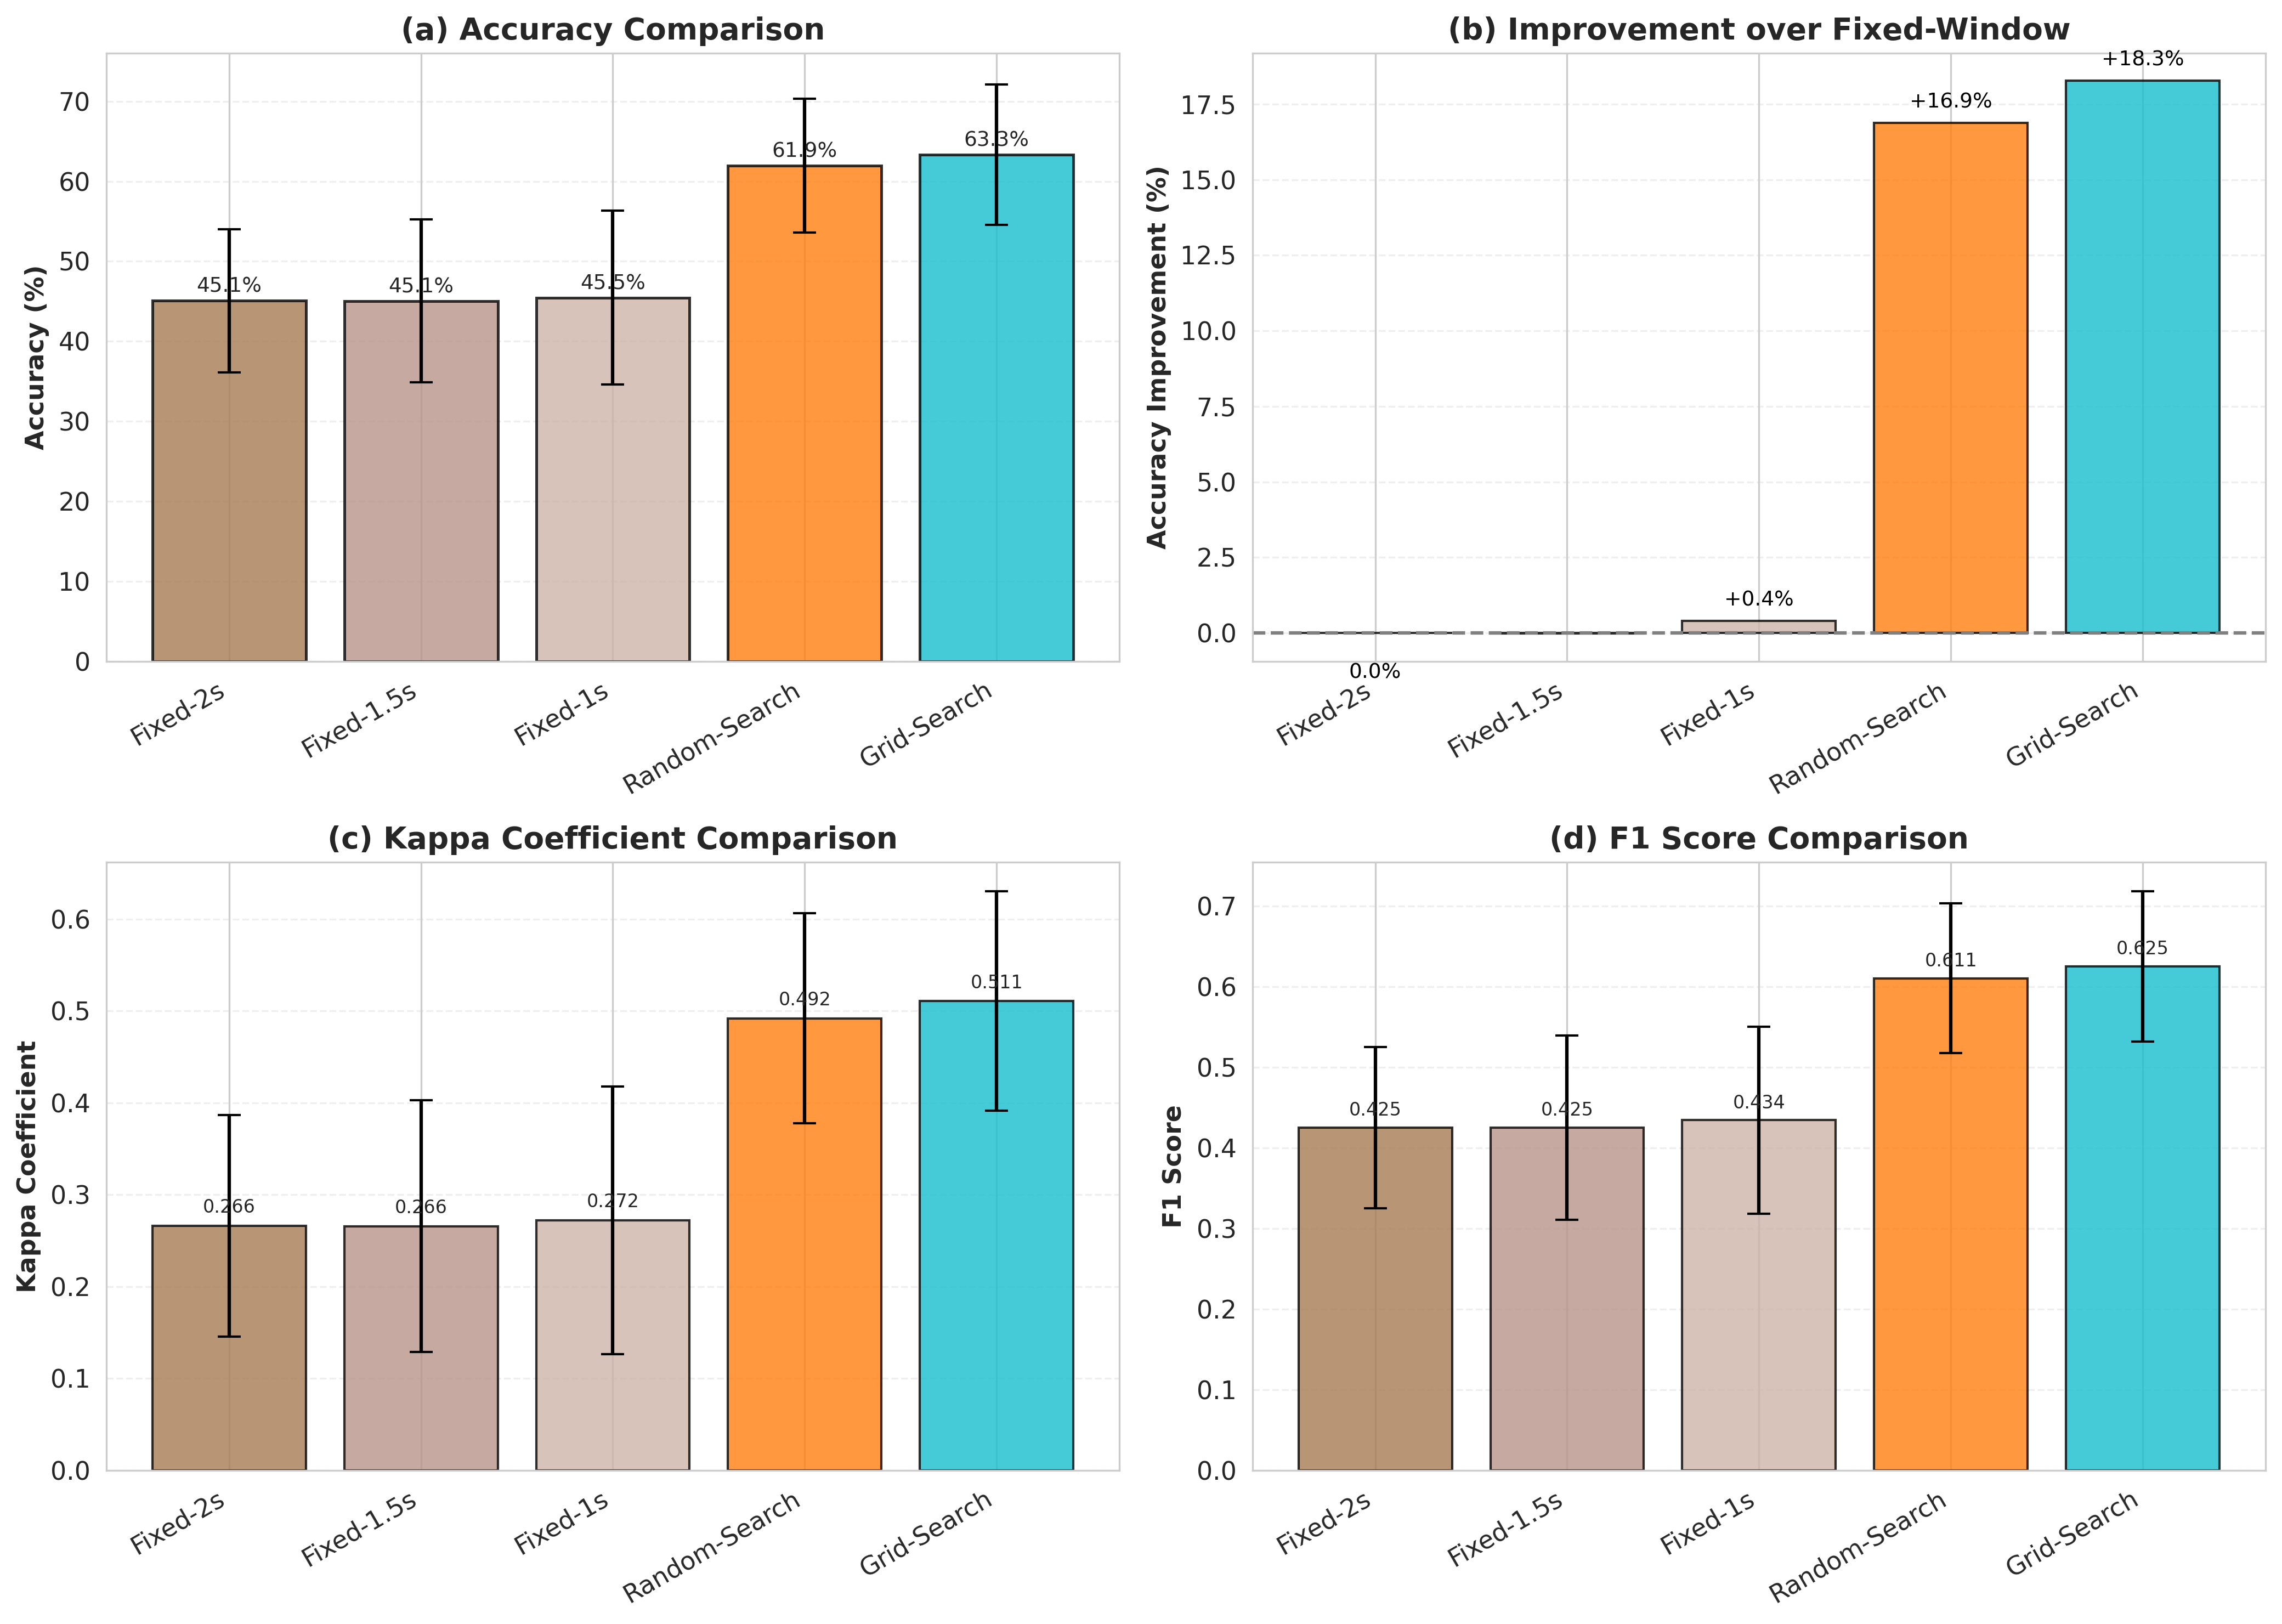
\includegraphics[width=0.85\textwidth]{figures/baseline/01_performance_comparison.png}
    \end{center}
\end{frame}

\begin{frame}{基线方法性能分析}
    \begin{alertblock}{主要发现}
        \footnotesize
        \begin{itemize}
            \item \textbf{准确率}：搜索策略 (61.9\%--63.3\%) 显著优于固定窗口 (约 45\%)
            \item \textbf{提升百分比}：Grid-Search 和 Random-Search 分别实现 +18.3\% 和 +16.9\%
            \item \textbf{Kappa 系数}：搜索策略 (0.49--0.51) 中等一致性，优于固定窗口 (0.27)
            \item \textbf{F1 分数}：搜索策略 (0.61--0.63) 较固定窗口 (0.43) 提升约 44\%
        \end{itemize}
    \end{alertblock}

    \vspace{0.2cm}
    \begin{exampleblock}{结果分析}
        \footnotesize
        搜索优化方法显著优于固定窗口策略。Grid-Search 准确率达 63.35\%，较 Fixed-2s 提升 18.3\%（相对提升 40.6\%）。Kappa 系数从 0.27 提升至 0.51，F1 分数从 0.43 提升至 0.63。这表明\textbf{自适应时间窗口能有效捕捉最优信号片段}，克服固定窗口无法适应 EEG 信号动态变化的局限。
    \end{exampleblock}
\end{frame}

\begin{frame}{基线方法稳定性分析}
    \begin{center}
    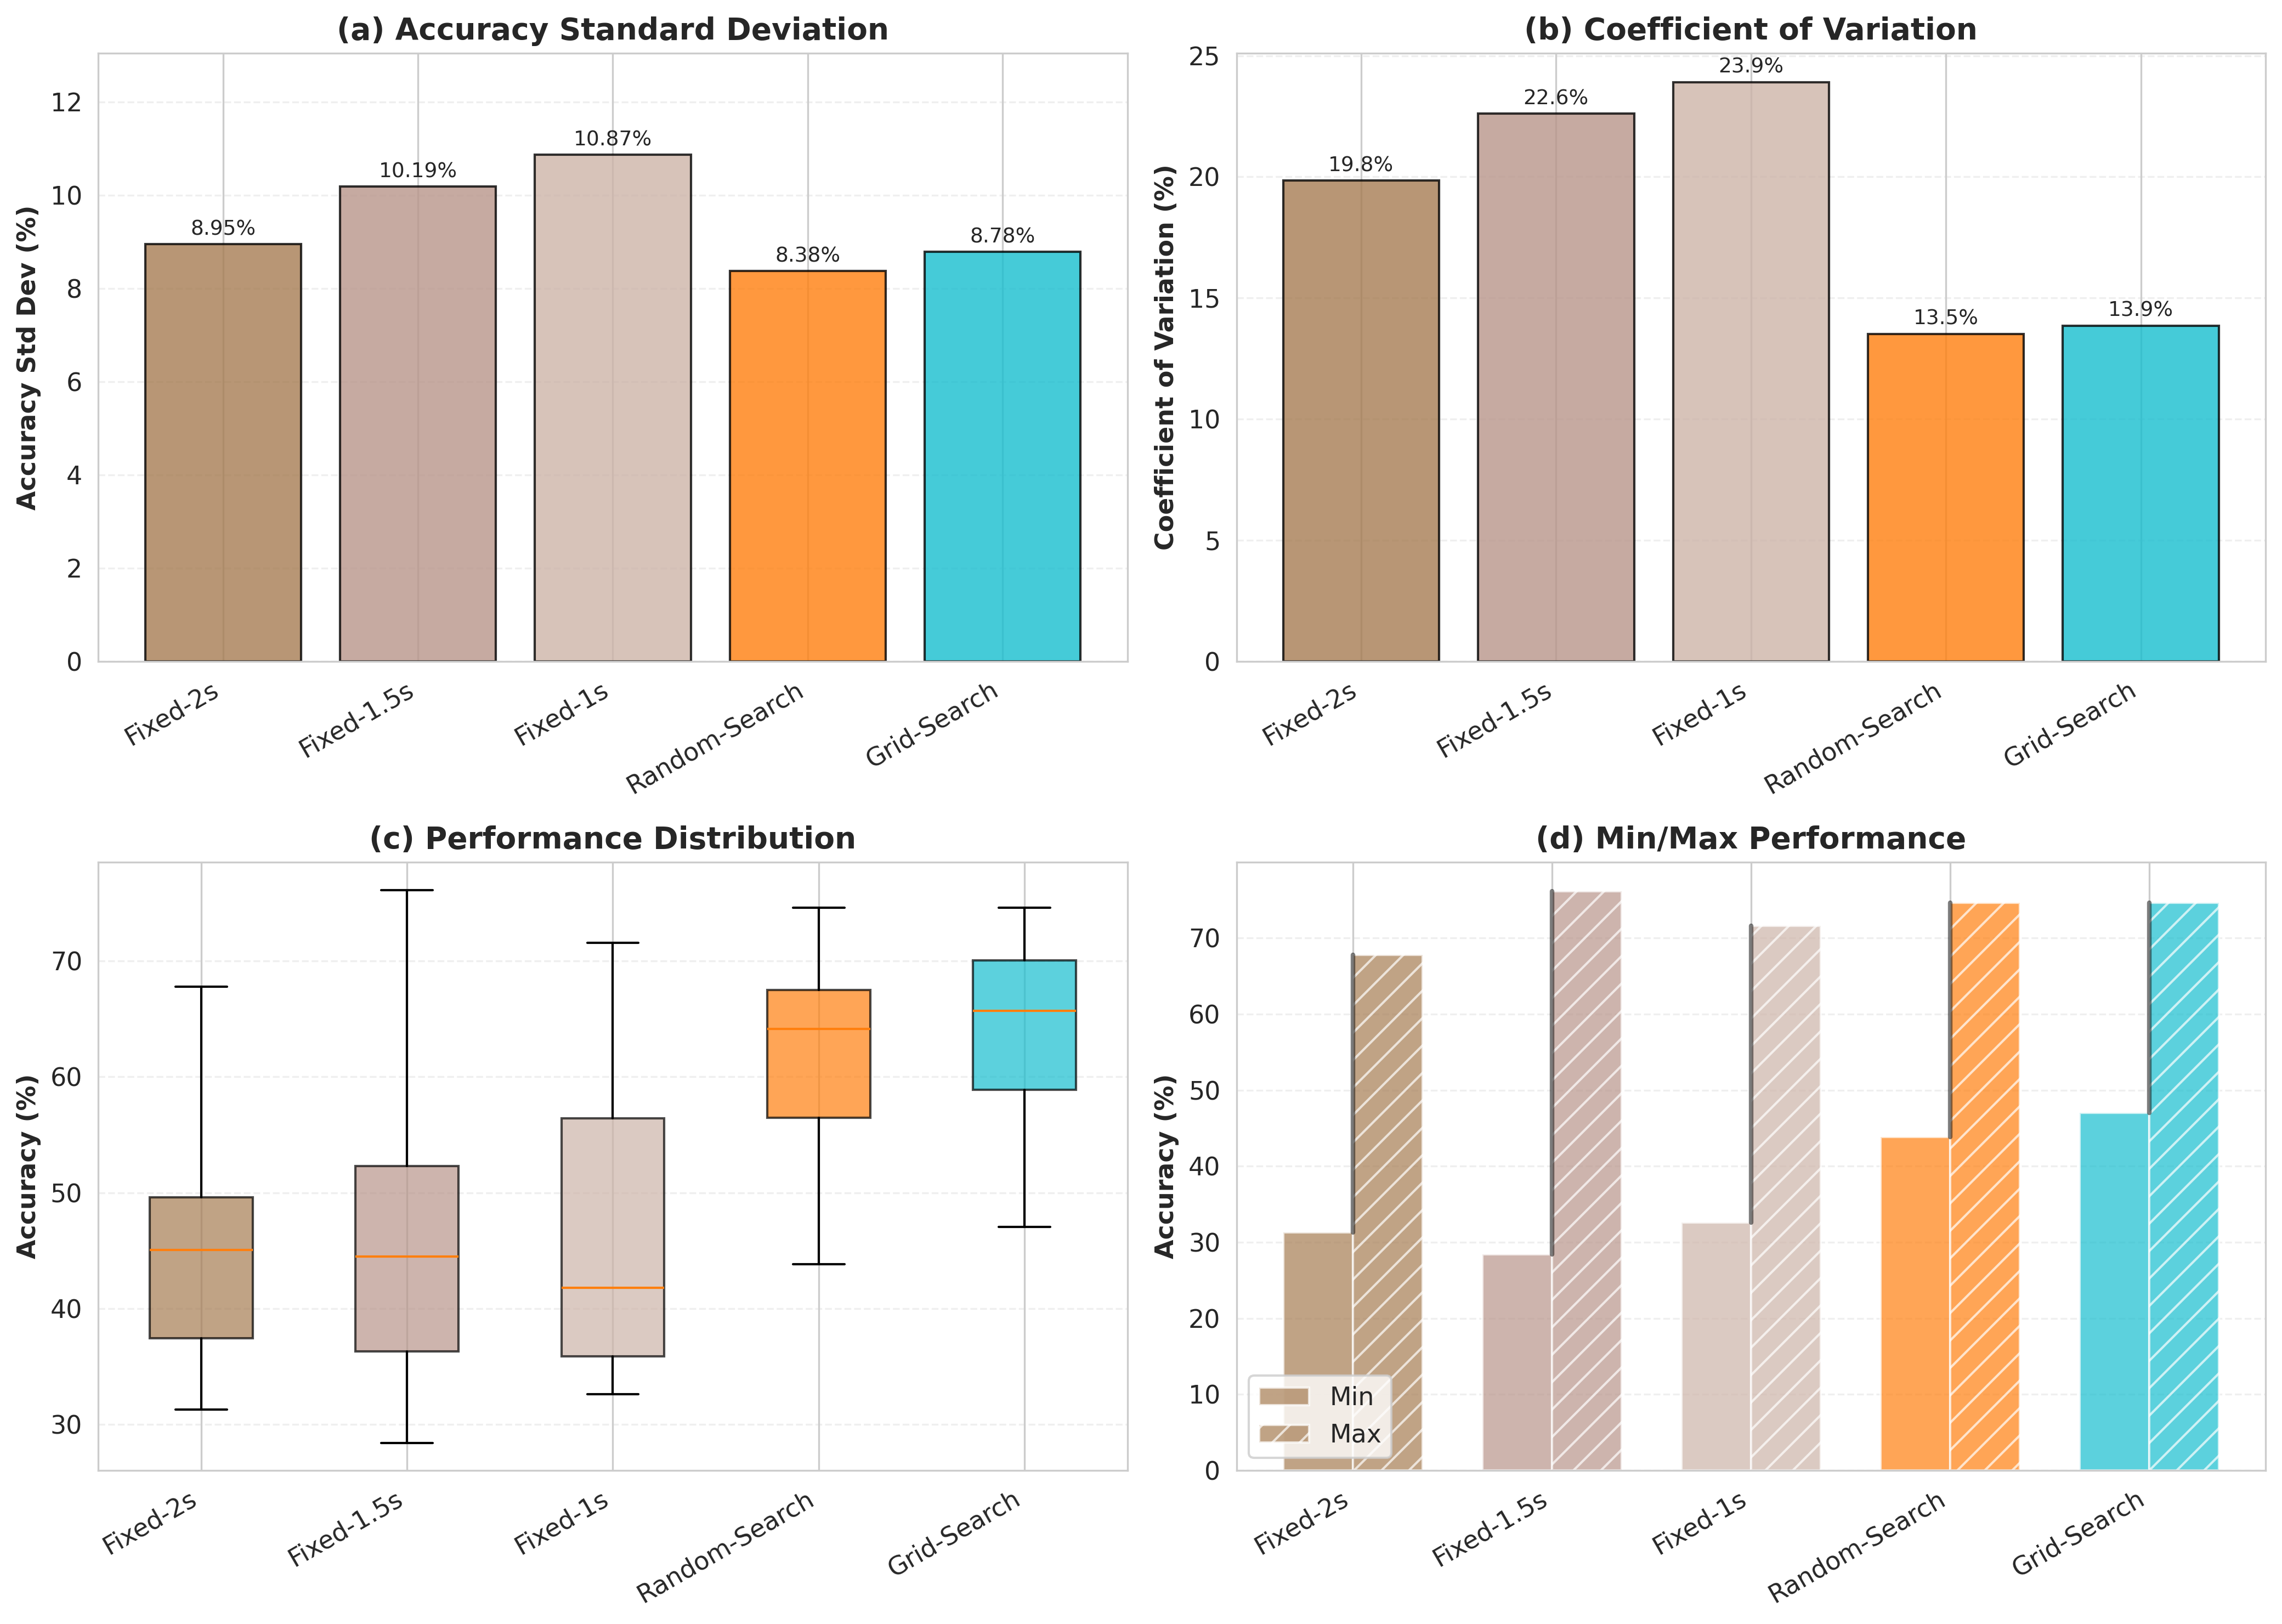
\includegraphics[width=0.85\textwidth]{figures/baseline/01_stability_analysis.png}
    \end{center}
\end{frame}

\begin{frame}{基线方法稳定性分析}
    \begin{exampleblock}{稳定性评估}
        \footnotesize
        \begin{itemize}
            \item \textbf{标准差}：搜索策略显著降低性能波动
            \item \textbf{变异系数}：搜索策略 (13.5\%--13.9\%) vs 固定窗口 (19.8\%--23.9\%)
            \item \textbf{最小准确率}：搜索方法 (约 47\%) 远高于固定窗口 (28\%--33\%)
            \item \textbf{结论}：搜索策略有效提升性能下限保障
        \end{itemize}
    \end{exampleblock}

    \vspace{0.2cm}
    \begin{alertblock}{结果分析}
        \footnotesize
        尽管搜索方法的绝对标准差与 Fixed-2s 相近，但其变异系数显著降低（13.5\%--13.9\% vs 19.8\%--23.9\%）。更重要的是，搜索方法的最小准确率（约 47\%）远高于固定窗口（约 28\%--33\%），\textbf{有效避免了极端差性能的出现}，提高了方法的下限保障。
    \end{alertblock}
\end{frame}

\begin{frame}{各被试准确率分布}
    \begin{center}
    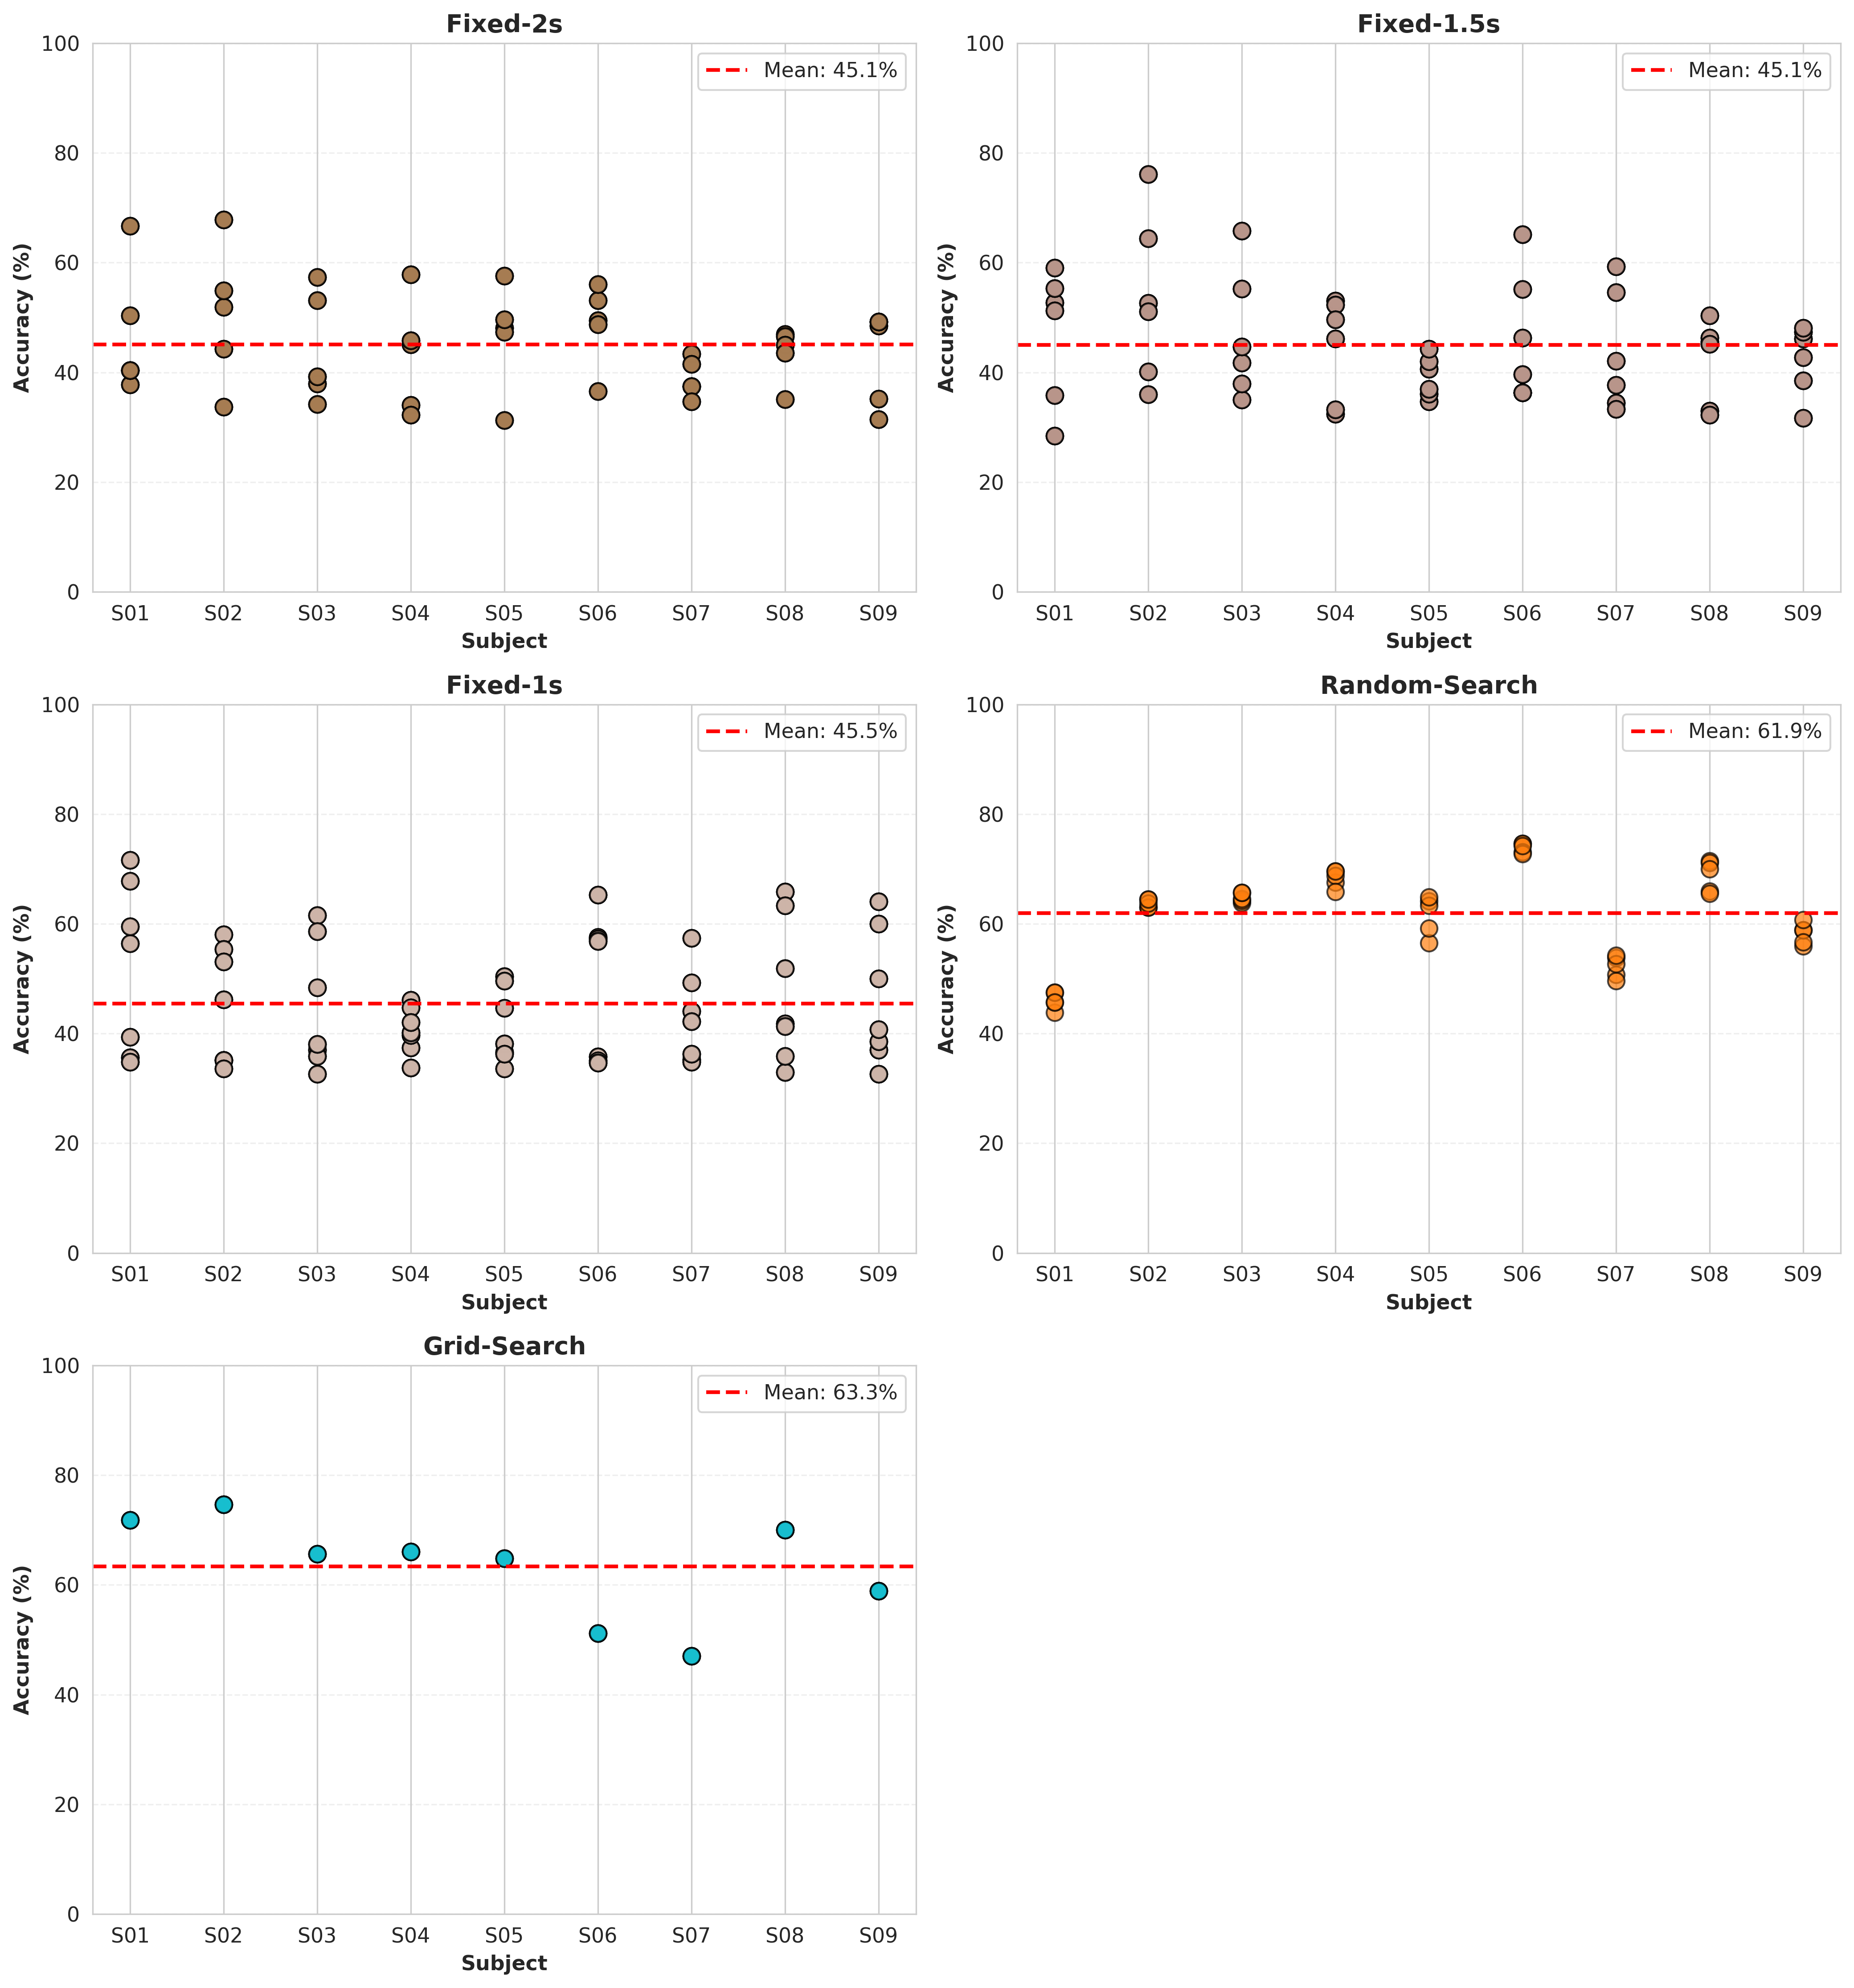
\includegraphics[width=0.6\textwidth]{figures/baseline/01_subject_distribution.png}
    \end{center}
\end{frame}

\begin{frame}{各被试准确率分布分析}
    \begin{alertblock}{个体差异分析}
        \footnotesize
        \begin{itemize}
            \item \textbf{固定窗口}：被试间差异大 (30\%--70\%)，平均停滞在 45\%
            \item \textbf{Random-Search}：同一被试多次运行高度聚集，均值提升至 61.9\%
            \item \textbf{Grid-Search}：最高平均准确率 63.3\%
            \item \textbf{结论}：搜索策略有效缓解个体差异带来的性能波动
        \end{itemize}
    \end{alertblock}

    \vspace{0.2cm}
    \begin{exampleblock}{结果分析}
        \footnotesize
        固定窗口方法在被试间表现出极大波动（30\%--70\%），而 Random-Search 在同一被试的多次运行中高度一致。这验证了\textbf{个体间神经响应模式的异质性}，搜索策略通过为每个样本独立优化窗口，有效适应了这种差异。
    \end{exampleblock}
\end{frame}

\begin{frame}{基线方法详细对比}
    \begin{center}
    \footnotesize
    \renewcommand{\arraystretch}{1.3}
    \begin{tabular}{lccccc}
        \hline
        \textbf{Method} & \textbf{Accuracy (\%)} & \textbf{Kappa} & \textbf{F1} & \textbf{Std Dev (\%)} & \textbf{CV (\%)} \\
        \hline
        Fixed-2s & 45.08 $\pm$ 8.95 & 0.266 & 0.426 & 8.95 & 19.85 \\
        Fixed-1.5s & 45.05 $\pm$ 10.19 & 0.266 & 0.425 & 10.19 & 22.61 \\
        Fixed-1s & 45.47 $\pm$ 10.87 & 0.272 & 0.434 & 10.87 & 23.91 \\
        Random-Search & 61.95 $\pm$ 8.38 & 0.492 & 0.611 & 8.38 & 13.52 \\
        Grid-Search & \textbf{63.35 $\pm$ 8.78} & \textbf{0.511} & \textbf{0.625} & 8.78 & 13.86 \\
        \hline
    \end{tabular}
    \end{center}
\end{frame}

\begin{frame}{基线方法结果分析}
    \begin{alertblock}{结果分析}
        \footnotesize
        \begin{itemize}
            \item Grid-Search 准确率达 63.35\%，较 Fixed-2s 提升 18.3\%
            \item Kappa 系数从 0.27 提升至 0.51，F1 从 0.43 提升至 0.63
            \item 搜索策略变异系数显著降低，有效避免极端差性能
        \end{itemize}
    \end{alertblock}

    \vspace{0.2cm}
    \begin{exampleblock}{搜索策略比较}
        \footnotesize
        Grid-Search 略优于 Random-Search（+1.4\%），但差异微小（< 2.3\%）。考虑到 Random-Search 的计算效率优势，\textbf{在实时 BCI 系统中可能更具实用价值}。三种固定窗口长度性能几乎相同（45.05\%--45.47\%），表明\textbf{简单调整窗口长度无法解决固定窗口的固有局限}，自适应策略是必然选择。
    \end{exampleblock}
\end{frame}

% ============================================================================
% Q-Learning 方法与基线方法对比
% ============================================================================
\subsection{Q-Learning 方法与基线方法对比}

\begin{frame}{Q-Learning 与基线方法性能对比}
    \begin{center}
    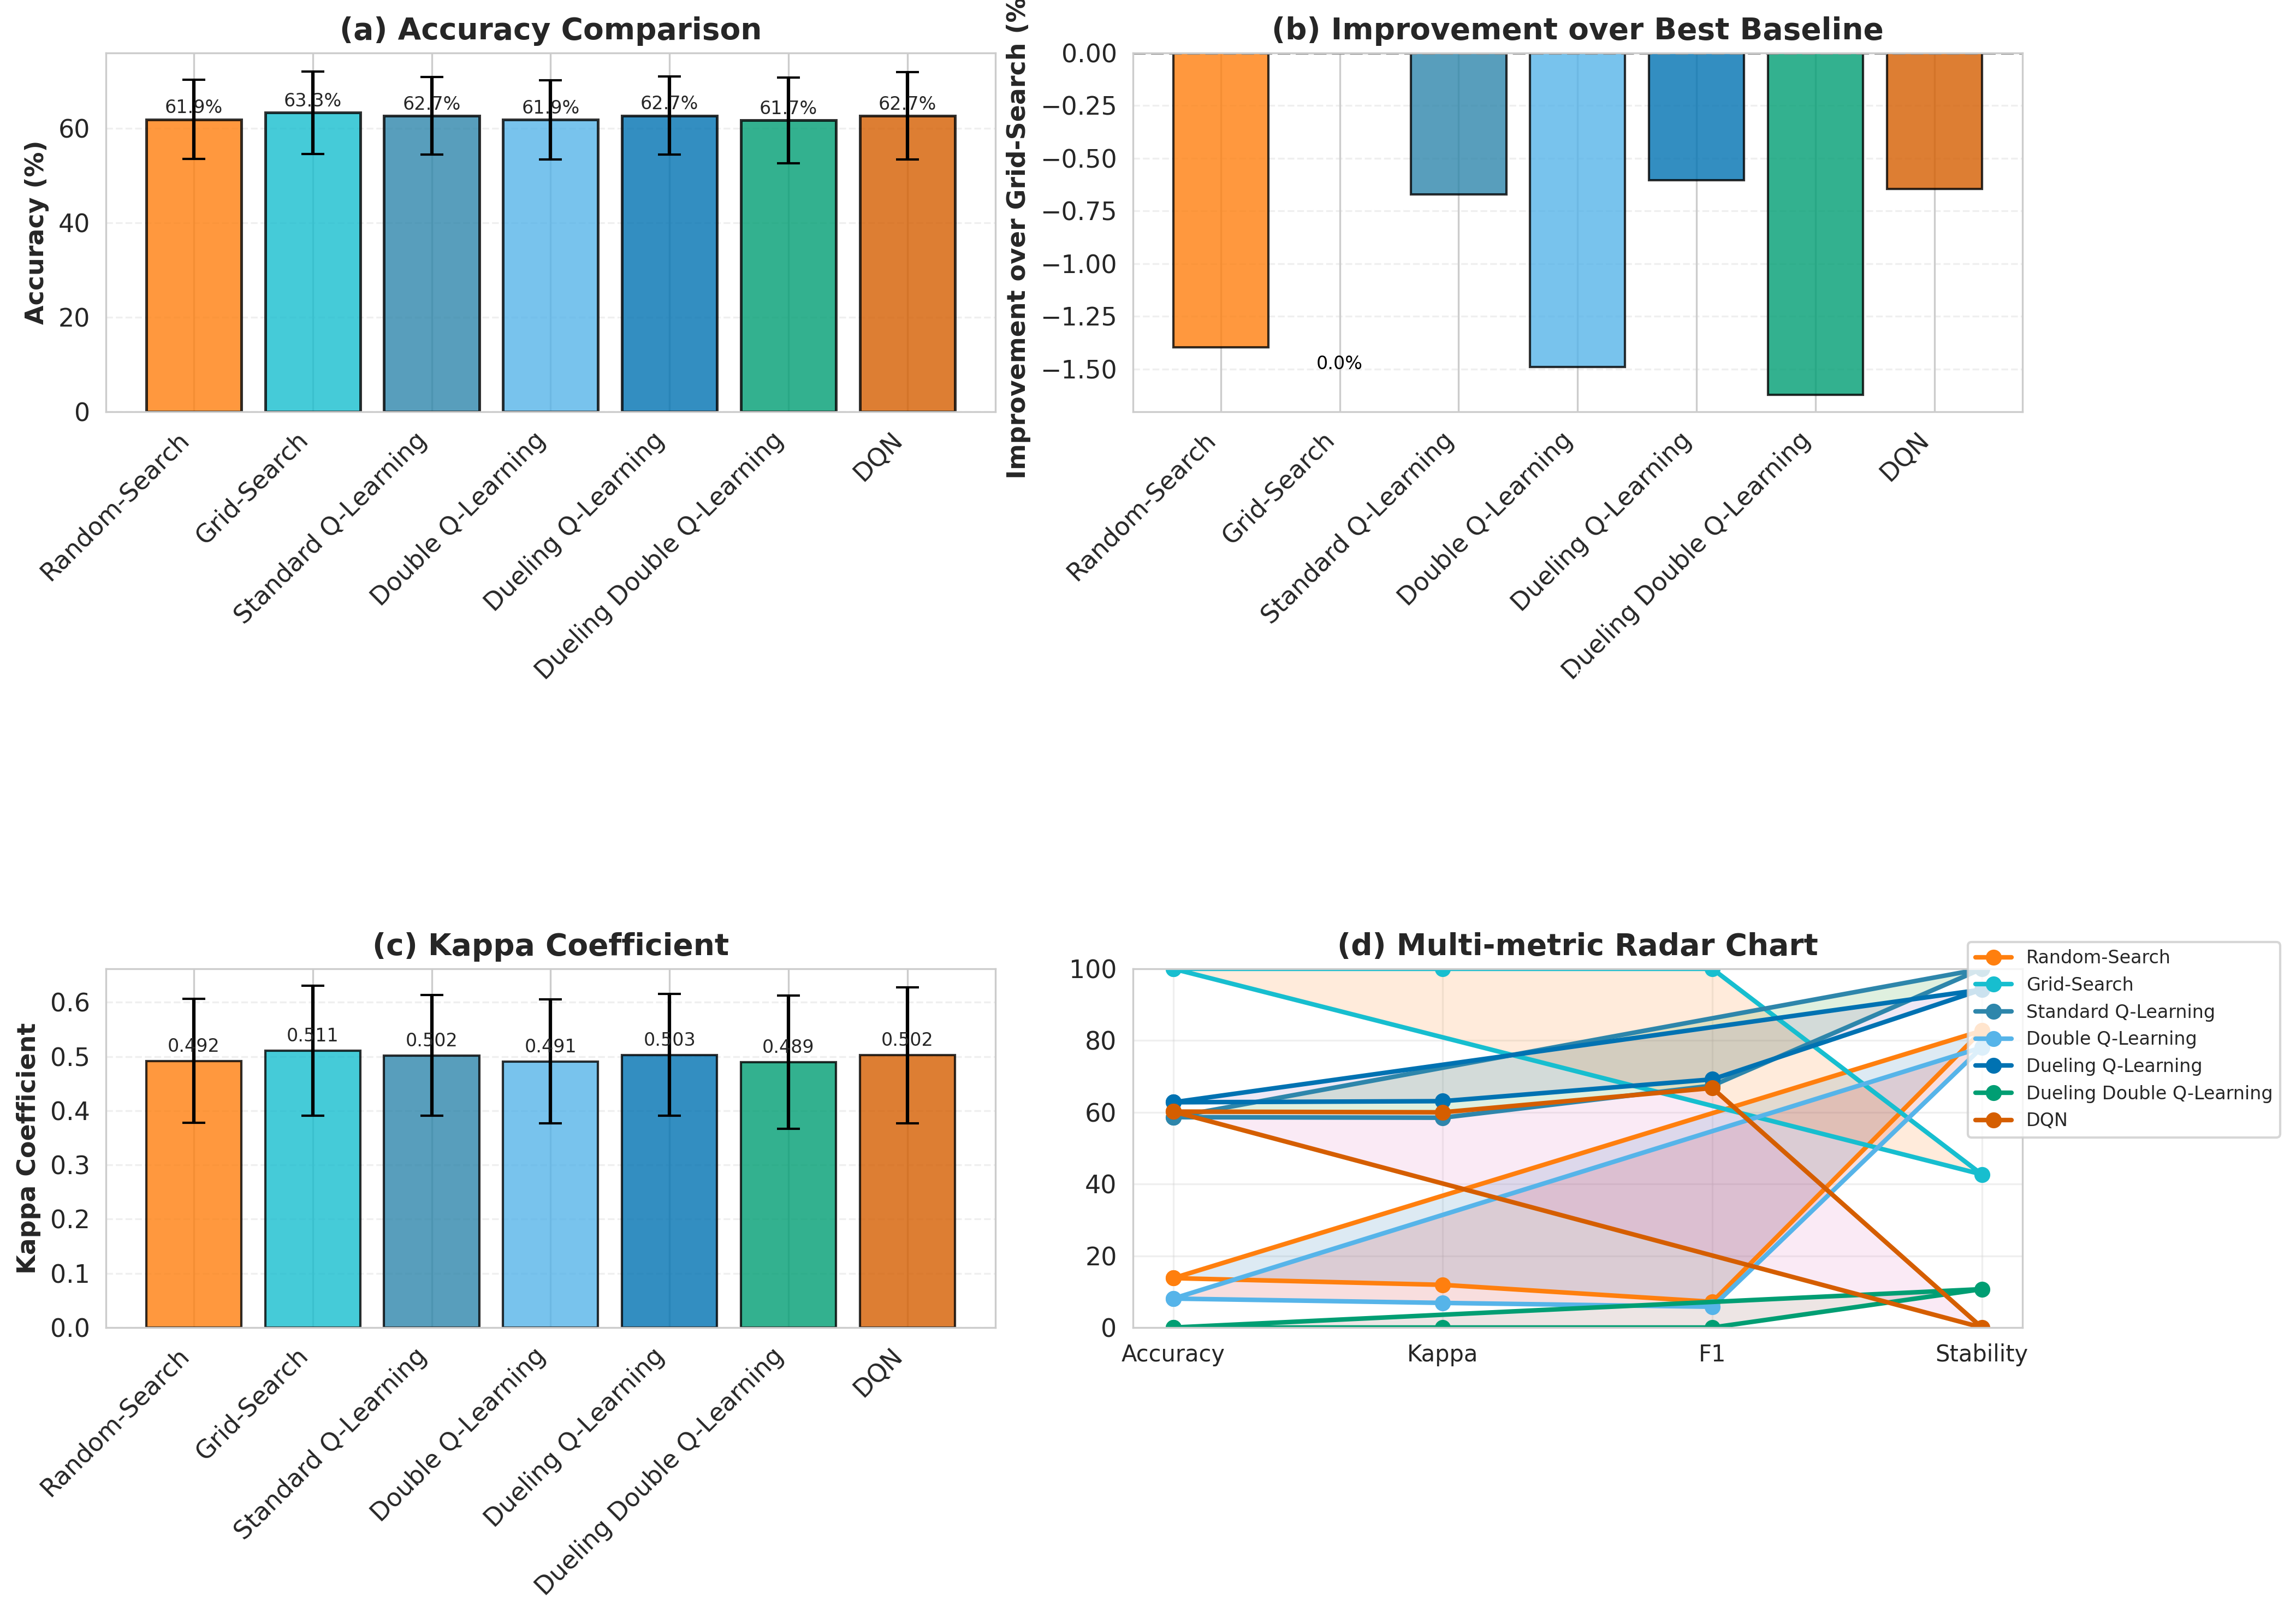
\includegraphics[width=0.85\textwidth]{figures/q_vs_baseline/02_performance_comparison.png}
    \end{center}
\end{frame}

\begin{frame}{Q-Learning 与基线方法性能分析}
    \begin{exampleblock}{性能对比}
        \footnotesize
        \begin{itemize}
            \item \textbf{准确率}：所有方法相近 (61.7\%--63.3\%)，Grid-Search 略居首位
            \item \textbf{相对改进}：强化学习方法略低于 Grid-Search (-0.6\% 至 -1.6\%)
            \item \textbf{Kappa 系数}：各方法集中在 0.49--0.51，一致性水平相当
            \item \textbf{雷达图}：Grid-Search 在准确率和 F1 最优，强化学习在稳定性略有优势
        \end{itemize}
    \end{exampleblock}

    \vspace{0.2cm}
    \begin{alertblock}{结果分析}
        \footnotesize
        Grid-Search 以 63.3\% 的准确率位居首位，所有强化学习方法的性能均略低于 Grid-Search（-0.6\% 至 -1.6\%），Random-Search 差距为 -1.4\%。各方法 Kappa 系数集中在 0.49--0.51 之间，分类一致性水平相当。实验结果表明，强化学习方法能够以较低的计算成本达到与网格搜索相近的性能水平，为实时自适应时间窗口选择提供了可行方案。
    \end{alertblock}
\end{frame}

\begin{frame}{统计显著性分析}
    \begin{center}
    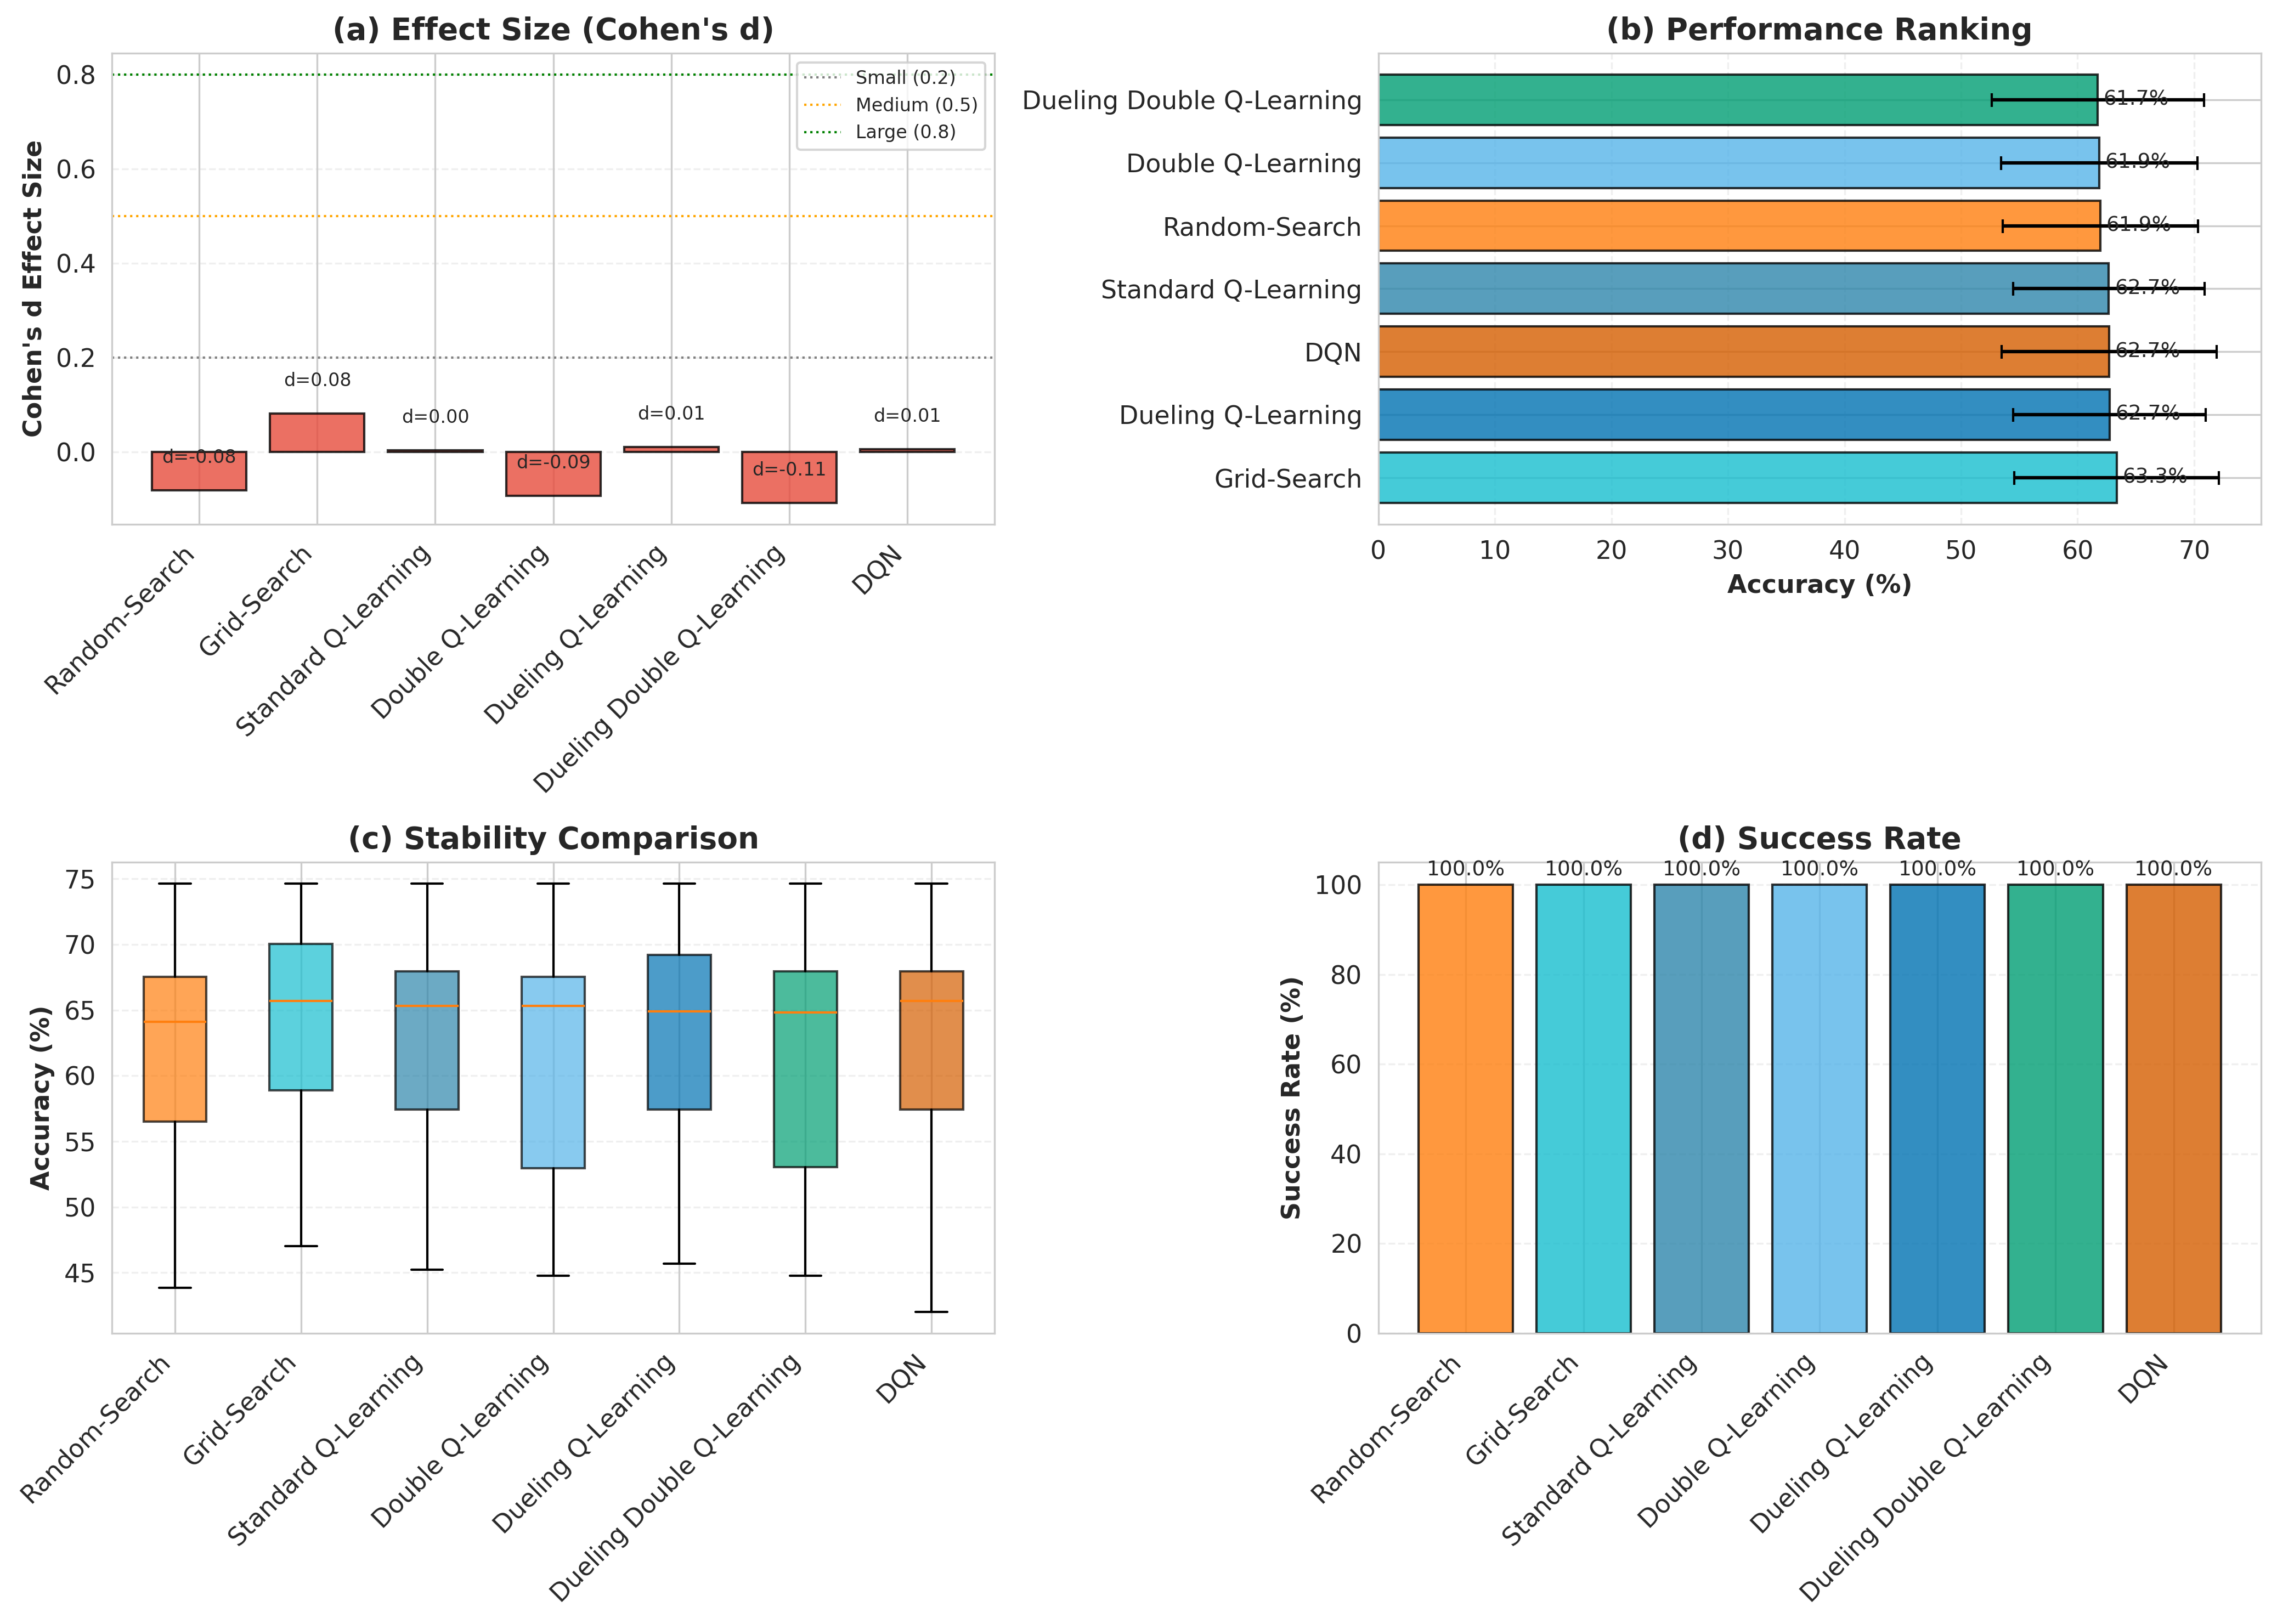
\includegraphics[width=0.85\textwidth]{figures/q_vs_baseline/02_statistical_analysis.png}
    \end{center}
\end{frame}

\begin{frame}{统计显著性分析}
    \begin{alertblock}{统计评估}
        \footnotesize
        \begin{itemize}
            \item \textbf{效应量}：所有方法效应量远小于小效应阈值 ($|d| < 0.2$)
            \item \textbf{性能排名}：Grid-Search (63.3\%) 第一，Q-Learning 变体 (62.7\%) 并列第二
            \item \textbf{稳定性}：各方法准确率分布范围相近 (45\%--75\%)
            \item \textbf{成功率}：所有方法均达 100\% 成功率
        \end{itemize}
    \end{alertblock}

    \vspace{0.2cm}
    \begin{exampleblock}{结果分析}
        \footnotesize
        所有 Q-Learning 方法与 Grid-Search 的 Cohen's d 值均远小于小效应阈值（$|d| < 0.2$），其中 Dueling Double Q-Learning 的效应量最大（$d=-0.11$）。这表明\textbf{尽管 Grid-Search 在数值上略优，但差异在统计学上不显著}，Q-Learning 方法可视为与 Grid-Search 性能等效。
    \end{exampleblock}
\end{frame}

\begin{frame}{时间窗选择模式分析}
    \begin{center}
    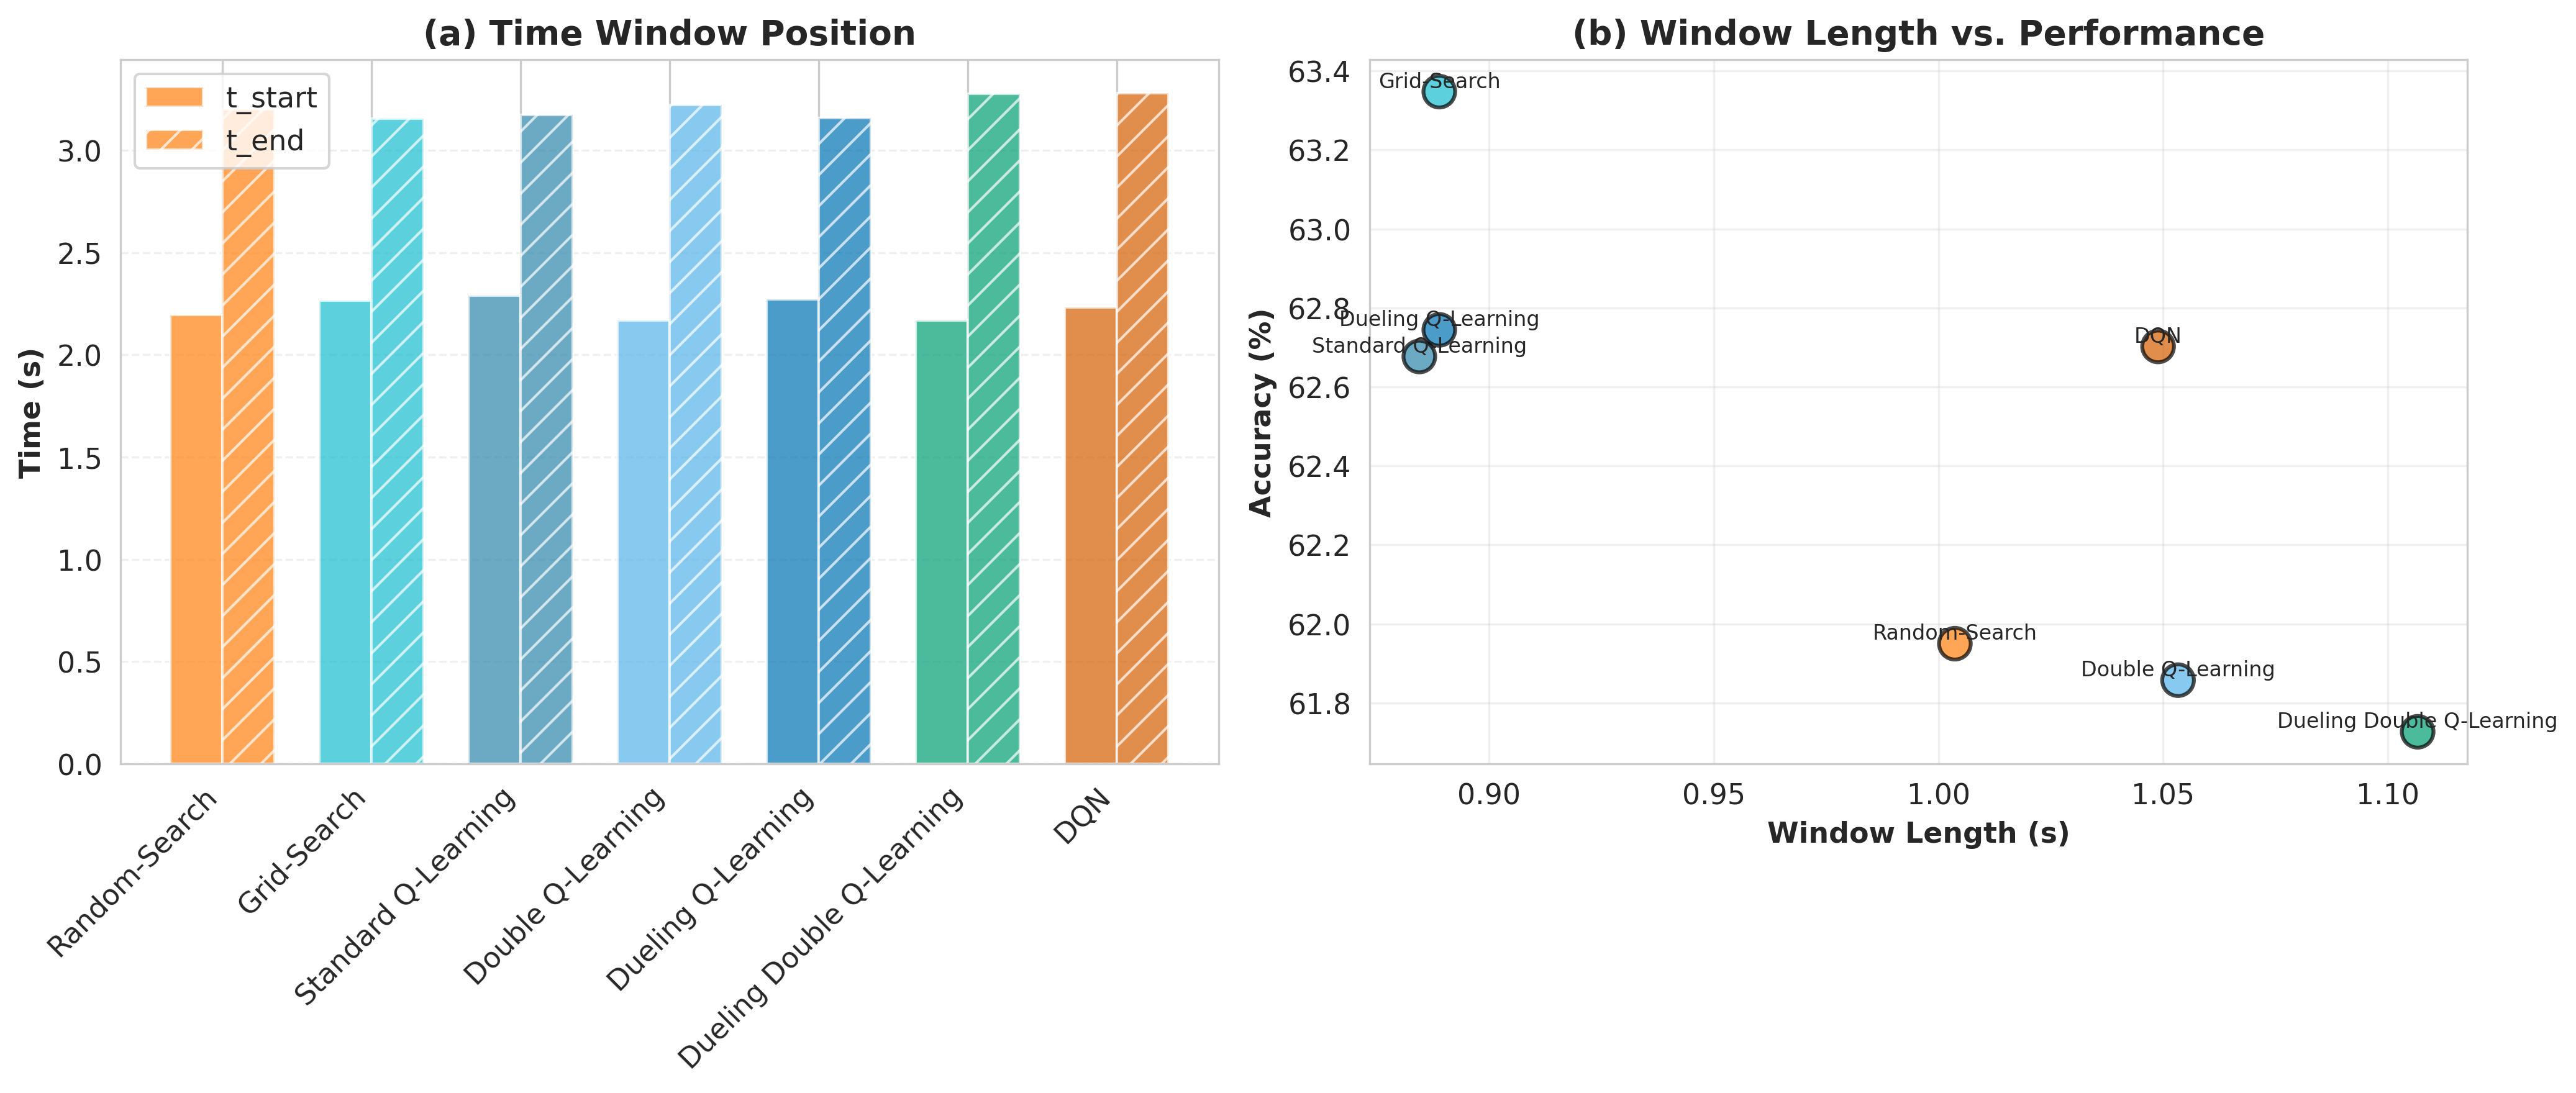
\includegraphics[width=0.85\textwidth]{figures/q_vs_baseline/02_window_performance.png}
    \end{center}
\end{frame}

\begin{frame}{时间窗选择模式分析}
    \begin{exampleblock}{时间窗分析}
        \footnotesize
        \begin{itemize}
            \item \textbf{位置分布}：所有方法倾向选择试验后期 ($t_{start} \approx 2.2$s, $t_{end} \approx 3.3$s)
            \item \textbf{关键发现}：运动想象关键神经特征主要分布在 trials 后半段
            \item \textbf{窗口长度与性能}：显著负相关，较短窗口 (约 0.9s) 准确率更高
            \item \textbf{结论}：精简时间窗口有助于减少噪声干扰并提升分类性能
        \end{itemize}
    \end{exampleblock}

    \vspace{0.2cm}
    \begin{alertblock}{结果分析}
        \footnotesize
        所有方法均倾向于选择试验后期的时间片段（$t_{start} \approx 2.2$s，$t_{end} \approx 3.3$s），验证了运动想象关键特征分布在 trials 后半段的假设。此外，窗口长度与性能呈负相关趋势，较短窗口（约 0.9s）比较长窗口（>1.0s）准确率更高，表明\textbf{精简窗口有助于减少噪声干扰}。Q-Learning 代理在训练过程中逐渐收敛至这一最优窗口范围，体现了其学习能力。
    \end{alertblock}
\end{frame}

\begin{frame}{Q-Learning 方法详细对比}
    \begin{center}
    \footnotesize
    \renewcommand{\arraystretch}{1.3}
    \begin{tabular}{lcccc}
        \hline
        \textbf{Method} & \textbf{Accuracy (\%)} & \textbf{Kappa} & \textbf{F1} & \textbf{Std Dev (\%)} \\
        \hline
        Random-Search & 61.95 $\pm$ 8.38 & 0.492 & 0.611 & 8.38 \\
        Grid-Search & \textbf{63.35 $\pm$ 8.78} & \textbf{0.511} & \textbf{0.625} & 8.78 \\
        Standard Q-Learning & 62.68 $\pm$ 8.20 & 0.502 & 0.620 & \textbf{8.20} \\
        Double Q-Learning & 61.86 $\pm$ 8.42 & 0.491 & 0.610 & 8.42 \\
        Dueling Q-Learning & 62.74 $\pm$ 8.26 & 0.503 & 0.620 & 8.26 \\
        Dueling Double Q-Learning & 61.73 $\pm$ 9.11 & 0.489 & 0.609 & 9.11 \\
        DQN & 62.70 $\pm$ 9.21 & 0.502 & 0.620 & 9.21 \\
        \hline
    \end{tabular}
    \end{center}
\end{frame}

\begin{frame}{Q-Learning 方法结果分析}
    \begin{alertblock}{结果分析}
        \footnotesize
        \begin{itemize}
            \item Standard Q-Learning 和 Dueling Q-Learning 表现最佳 (62.7\%)
            \item 与 Grid-Search 差距仅 0.6\%--1.6\%，统计上不显著
            \item Standard Q-Learning 稳定性最优 (Std Dev = 8.20\%)
        \end{itemize}
    \end{alertblock}

    \vspace{0.2cm}
    \begin{exampleblock}{稳定性与计算效率}
        \footnotesize
        从标准差来看，Standard Q-Learning（8.20\%）和 Dueling Q-Learning（8.26\%）的稳定性略优于 Grid-Search（8.78\%）和 Random-Search（8.38\%）。更重要的是，Q-Learning 方法在推理阶段仅需单次前向传播即可确定时间窗口，而 Grid-Search 需要遍历所有候选窗口组合。考虑到两者性能差异不显著（$< 1.6\%$），\textbf{Q-Learning 方法在实时 BCI 系统中具有明显的计算效率优势}。
    \end{exampleblock}
\end{frame}

% ============================================================================
% 表格型 Q-Learning 与 DQN 对比
% ============================================================================
\subsection{表格型 Q-Learning 与 DQN 对比}

\begin{frame}{Q-Learning 变体性能对比}
    \begin{center}
    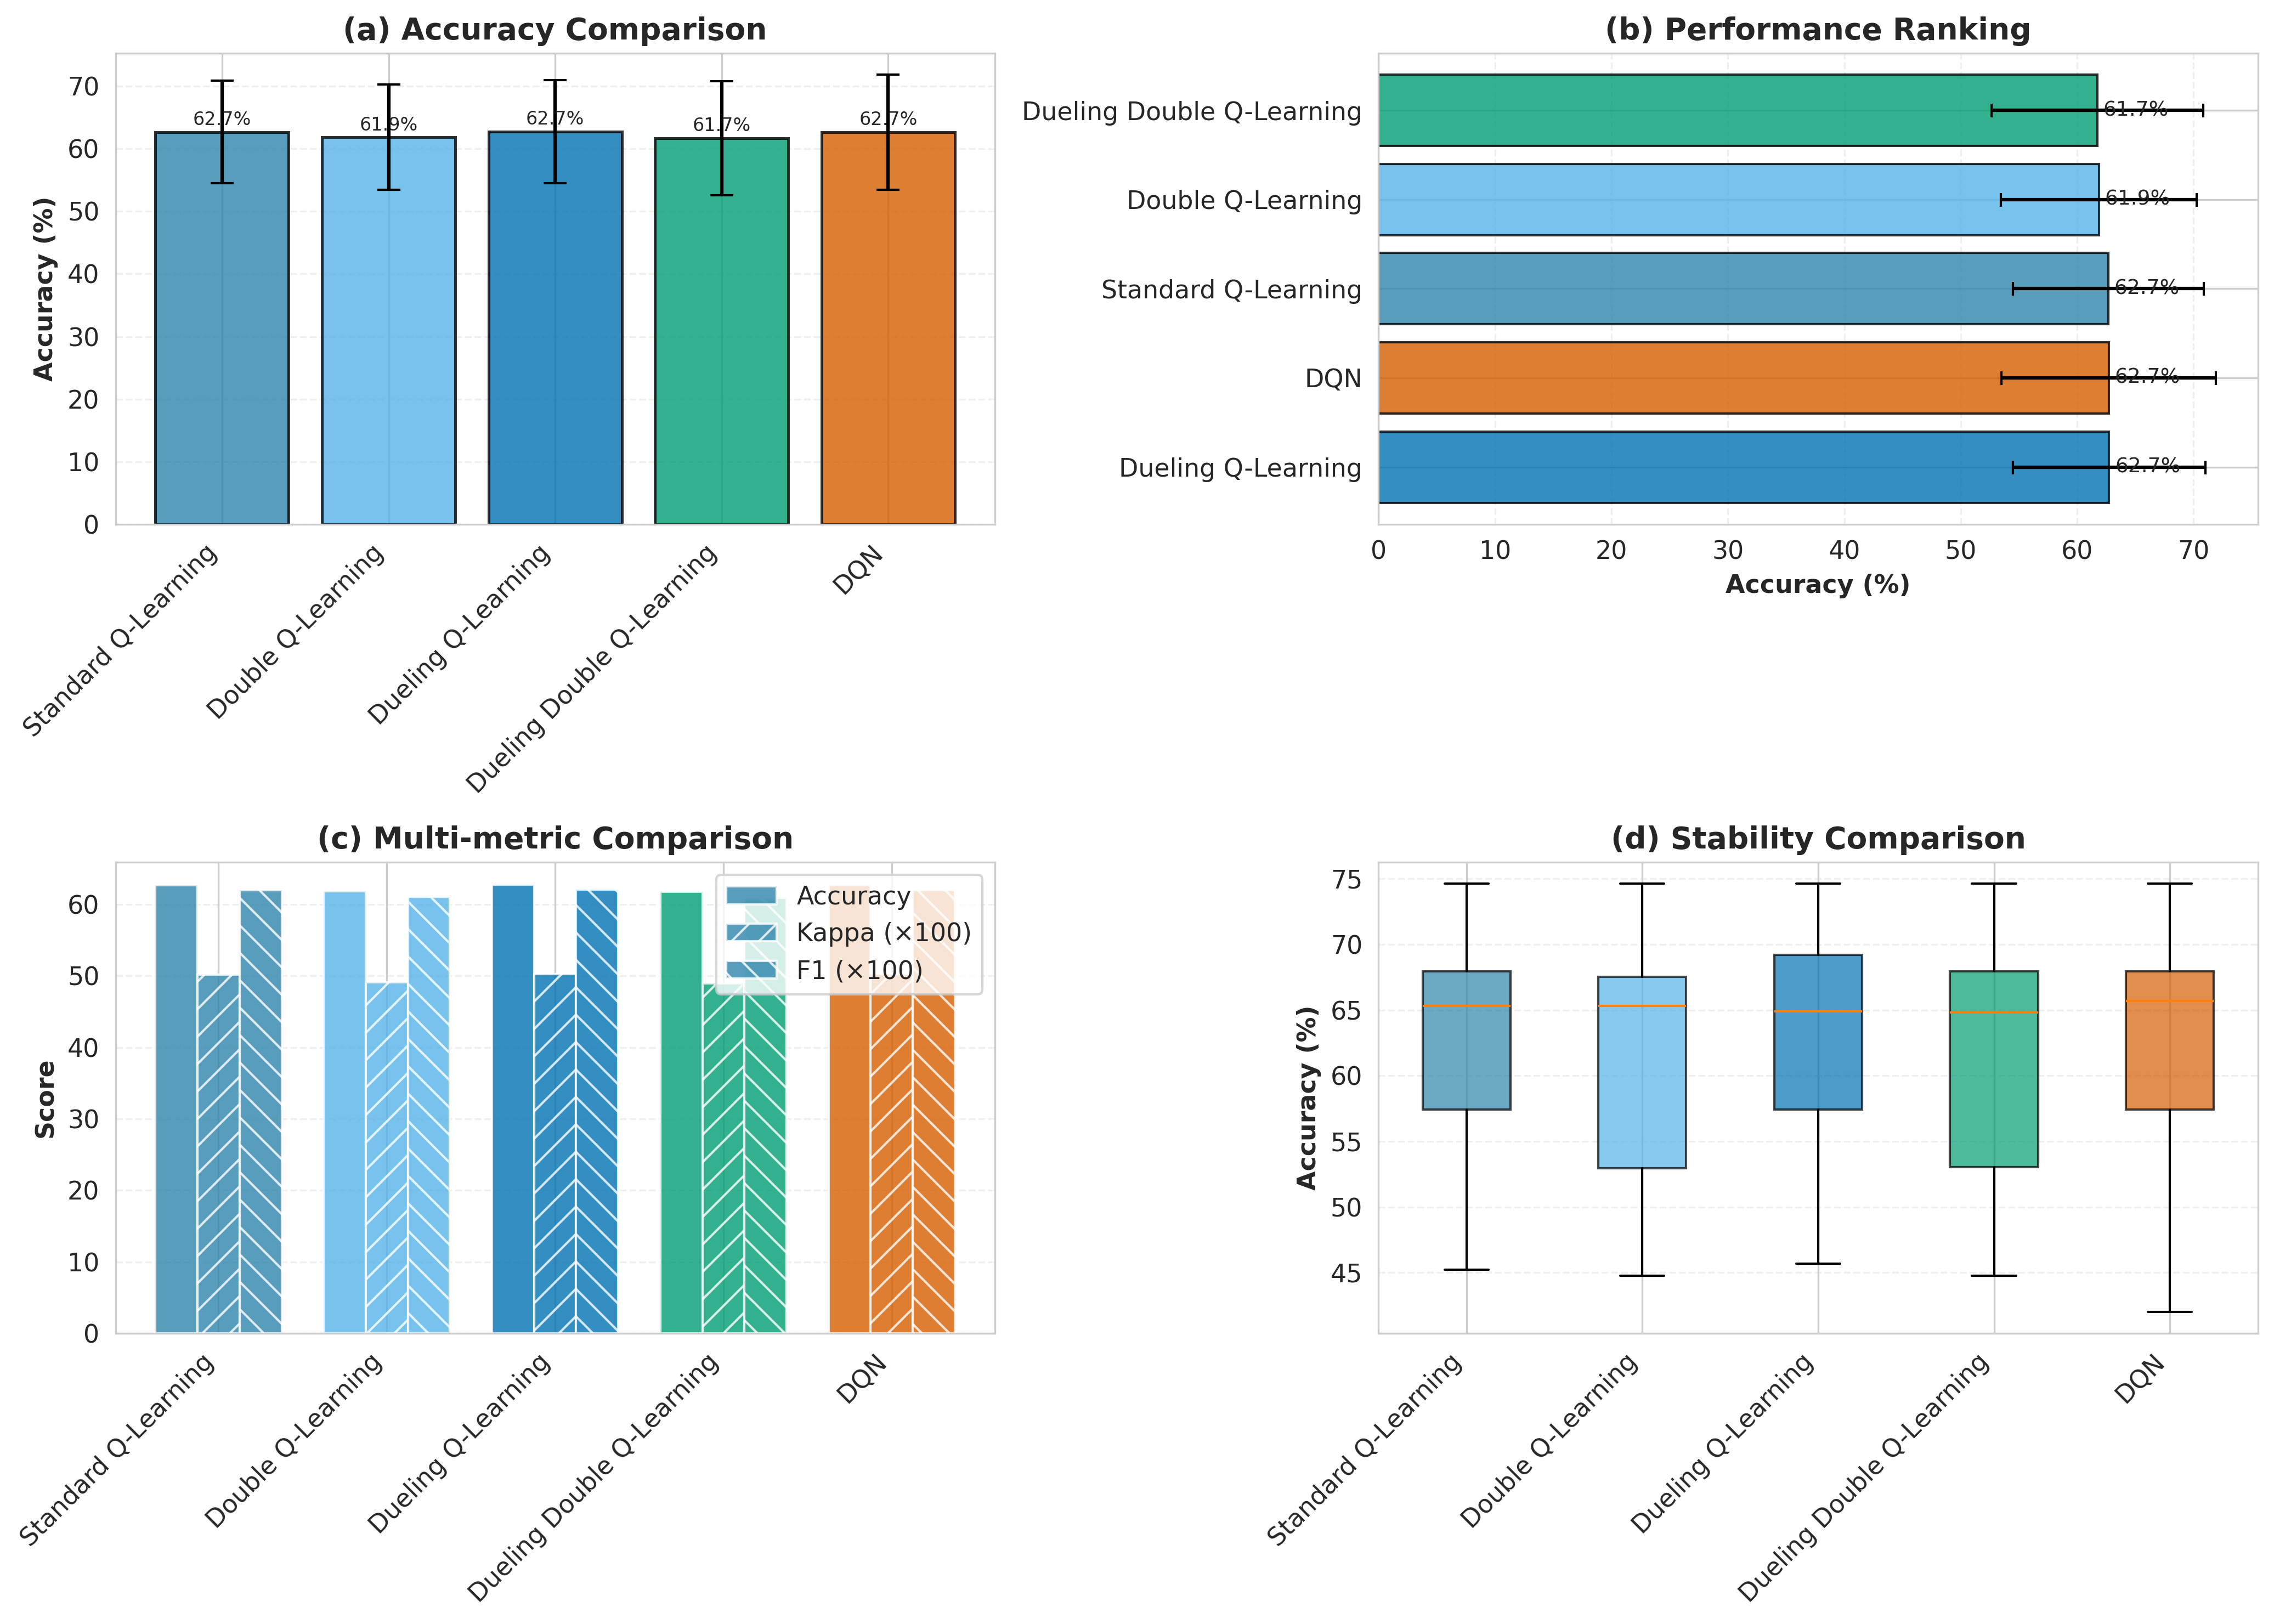
\includegraphics[width=0.85\textwidth]{figures/q_internal/03_performance_comparison.png}
    \end{center}
\end{frame}

\begin{frame}{Q-Learning 变体性能分析}
    \begin{exampleblock}{变体对比}
        \footnotesize
        \begin{itemize}
            \item \textbf{准确率}：各变体高度接近 (61.7\%--62.7\%)
            \item \textbf{最佳性能}：Standard Q-Learning、Dueling Q-Learning 和 DQN 并列 (62.7\%)
            \item \textbf{多指标}：所有变体在准确率、Kappa、F1 上表现一致
            \item \textbf{结论}：Standard Q-Learning 已足以捕捉策略，复杂变体未带来显著增益
        \end{itemize}
    \end{exampleblock}

    \vspace{0.2cm}
    \begin{alertblock}{结果分析}
        \footnotesize
        各变体性能高度接近（61.7\%--62.7\%），Standard Q-Learning、Dueling Q-Learning 和 DQN 并列最佳（62.7\%）。性能排名进一步确认了 Standard Q-Learning 等三种方法的领先地位，Dueling Double Q-Learning 略低（61.7\%）。多指标综合对比显示，所有变体在各项指标上表现一致，未见特定变体在某项指标上有显著优势。结果表明，在本任务中，\textbf{Standard Q-Learning 已足以捕捉时间窗口选择的策略，复杂的变体改进并未带来显著的性能增益}。
    \end{alertblock}
\end{frame}

\begin{frame}{Table Q-Learning 与 DQN 深度对比}
    \begin{center}
    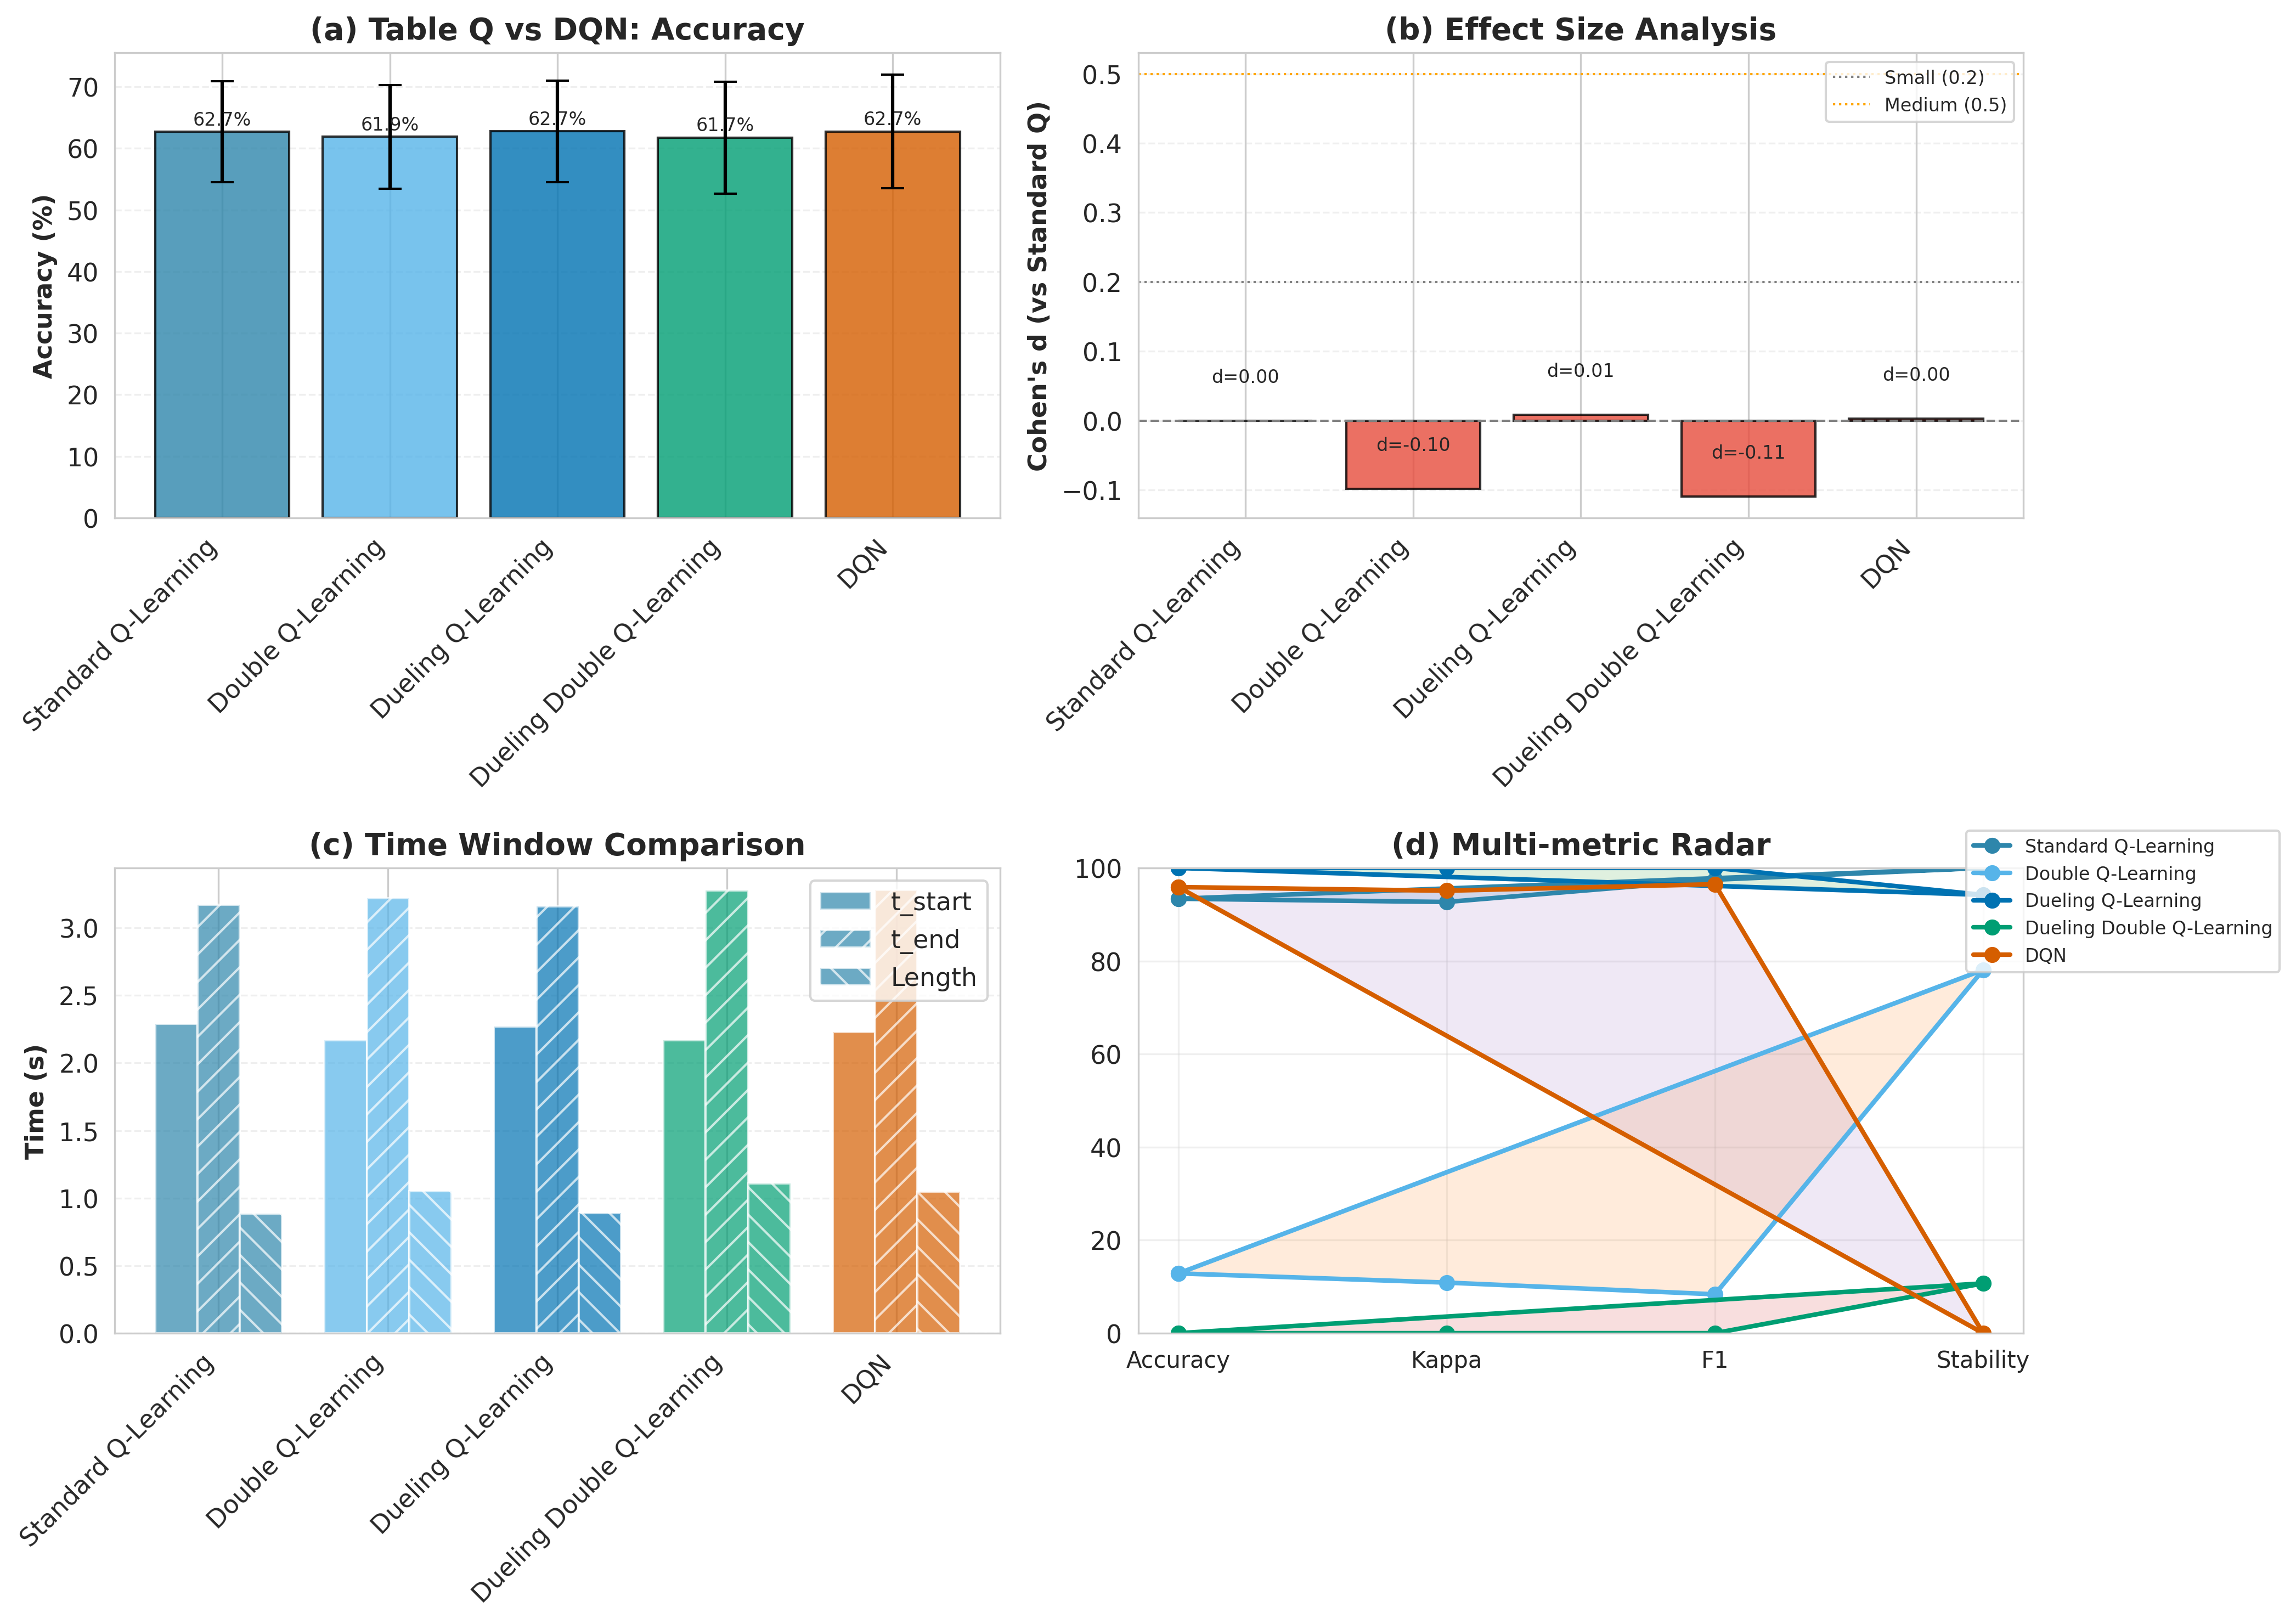
\includegraphics[width=0.85\textwidth]{figures/q_internal/03_table_q_vs_dqn.png}
    \end{center}
\end{frame}

\begin{frame}{Table Q-Learning 与 DQN 深度对比分析}
    \begin{alertblock}{深度对比}
        \footnotesize
        \begin{itemize}
            \item \textbf{准确率}：所有方法高度接近 (61.7\%--62.7\%)
            \item \textbf{效应量}：所有 $|d| < 0.2$，Standard Q 与 DQN 几乎无差异 ($d=0.00$)
            \item \textbf{时间窗}：DQN 选较短窗口 (约 1.0s)，Table Q 分布在 0.9s--1.1s
            \item \textbf{结论}：简单 Table Q-Learning 与复杂 DQN 性能相当
        \end{itemize}
    \end{alertblock}

    \vspace{0.2cm}
    \begin{exampleblock}{结果分析}
        \footnotesize
        所有方法性能高度接近（61.7\%--62.7\%），Standard Q-Learning、Dueling Q-Learning 和 DQN 均达到 62.7\% 的最高准确率。效应量分析显示，所有方法的效应量均远低于小效应阈值（$|d| < 0.2$），其中 Double Q-Learning ($d=-0.10$) 和 Dueling Double Q-Learning ($d=-0.11$) 显示出微小的负效应。结果表明，\textbf{在本任务中，简单的 Table Q-Learning 与复杂的 DQN 性能相当}，说明状态空间离散化策略已足够有效。
    \end{exampleblock}
\end{frame}

\begin{frame}{训练收敛特性分析}
    \begin{center}
    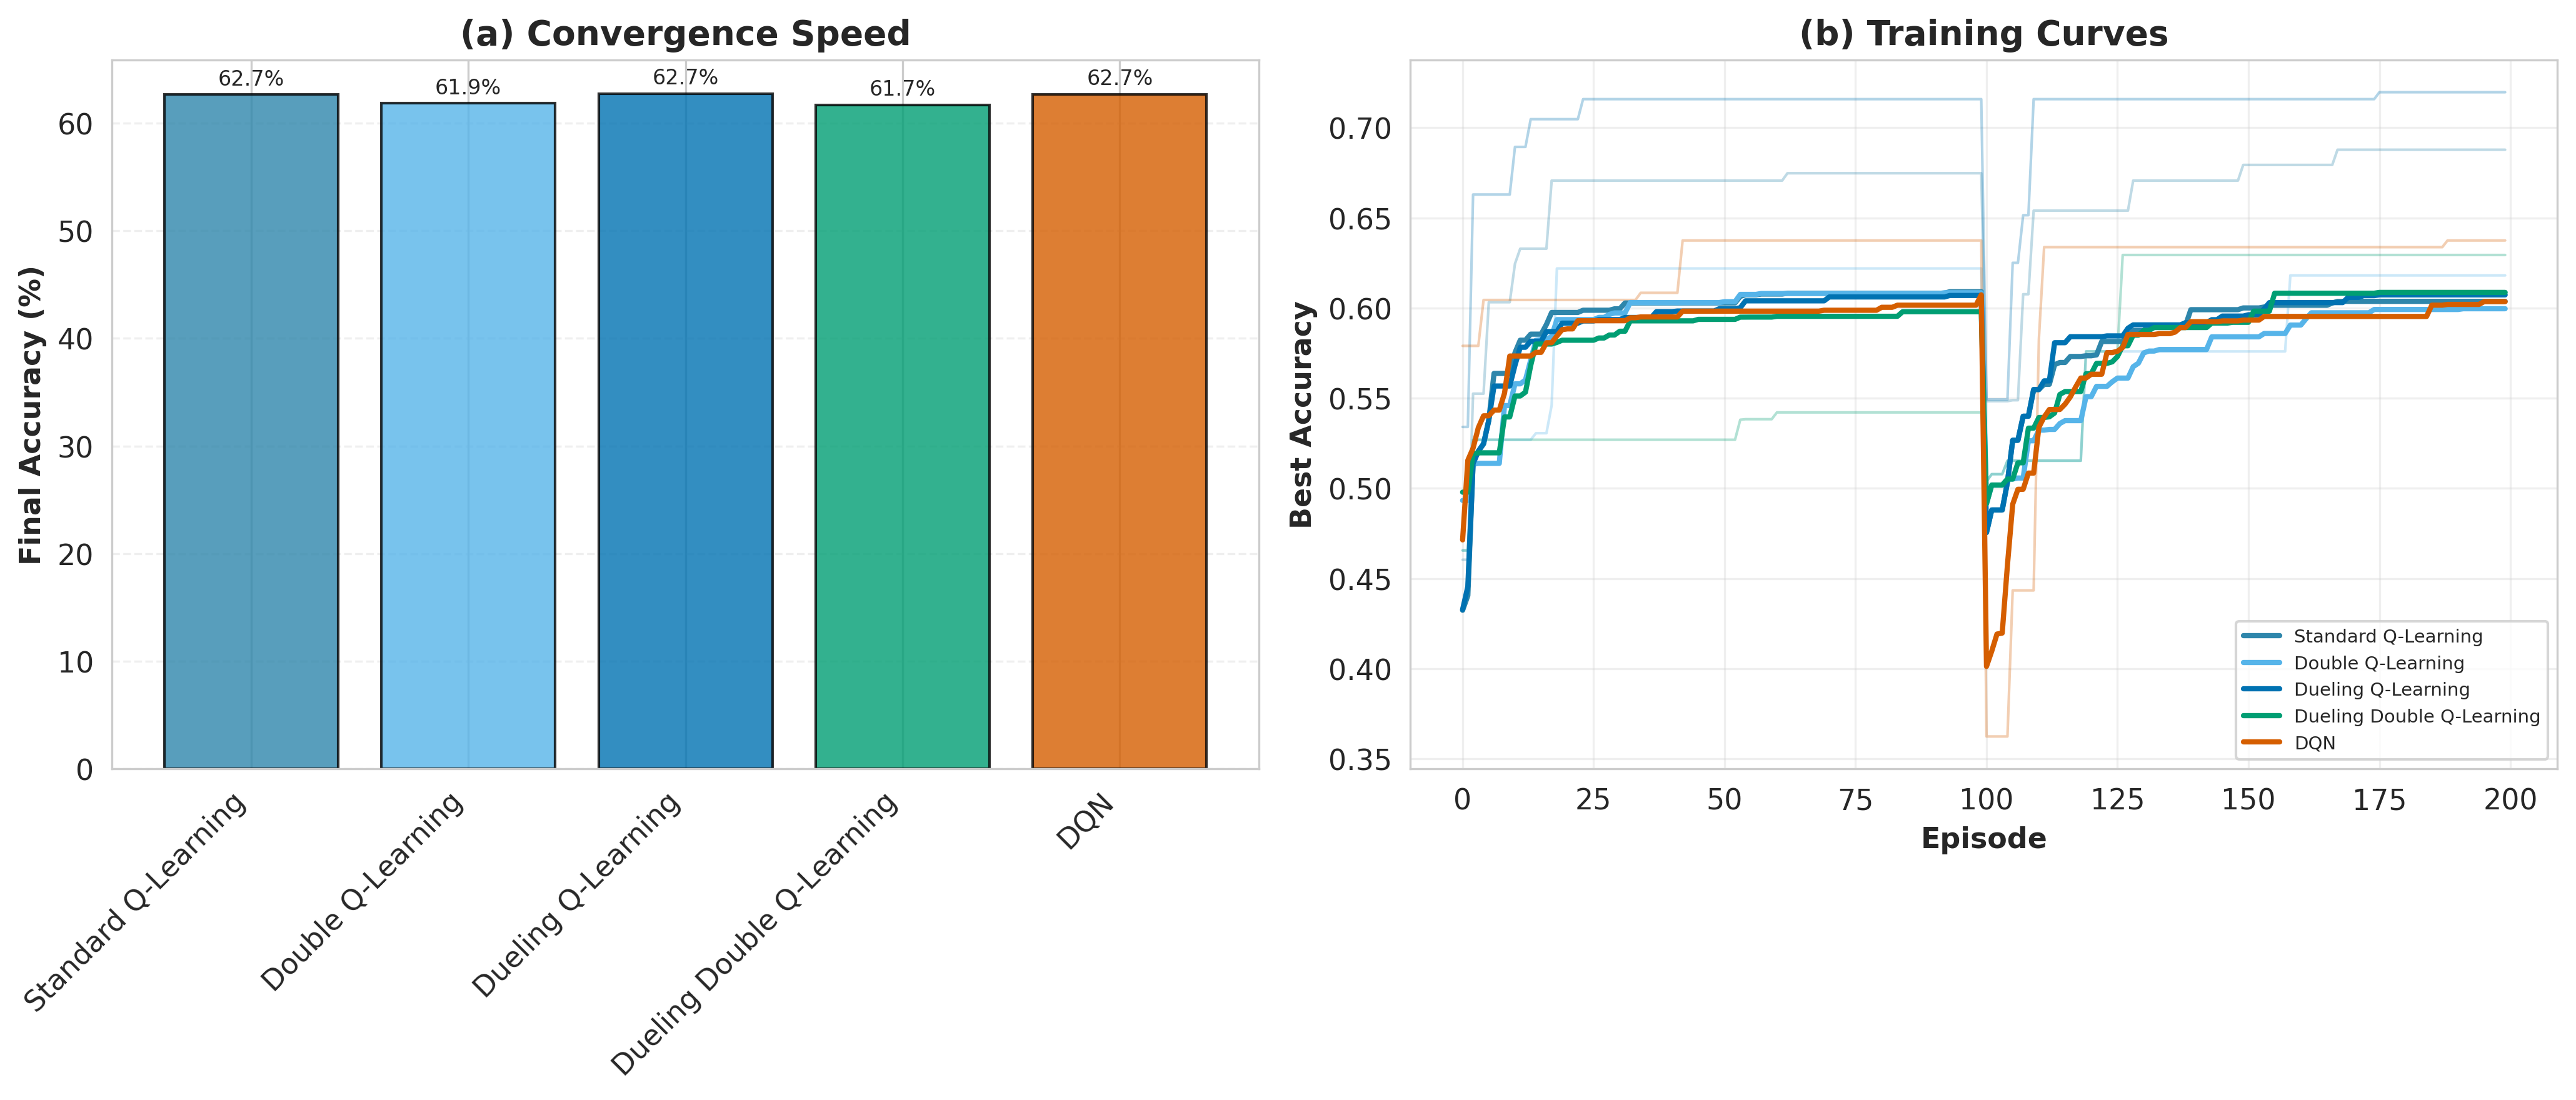
\includegraphics[width=0.85\textwidth]{figures/q_internal/03_training_performance.png}
    \end{center}
\end{frame}

\begin{frame}{训练收敛特性分析}
    \begin{exampleblock}{训练动态}
        \footnotesize
        \begin{itemize}
            \item \textbf{最终准确率}：Standard Q-Learning、Dueling Q-Learning 和 DQN 均达 62.7\%
            \item \textbf{收敛速度}：所有方法在 0--50 Episodes 快速收敛至 60\%
            \item \textbf{训练方差}：Double Q-Learning 方差大，Standard Q-Learning 和 DQN 更稳定
            \item \textbf{结论}：Standard Q-Learning 保持高性能同时，具有更优训练稳定性
        \end{itemize}
    \end{exampleblock}

    \vspace{0.2cm}
    \begin{alertblock}{结果分析}
        \footnotesize
        所有方法在初始阶段（0--50 Episodes）均表现出快速收敛特性，准确率迅速攀升至 60\% 左右。在 Episode 100 处观察到的性能波动后，各方法均能迅速恢复并趋于稳定。观察发现，Double Q-Learning 显示出较大的训练方差（细线离散度高），而 Standard Q-Learning 和 DQN 表现出更平滑、稳定的收敛过程。结果表明，Standard Q-Learning 在保持高性能的同时，具有更优的训练稳定性和收敛效率。
    \end{alertblock}
\end{frame}

\begin{frame}{Table Q-Learning vs DQN 详细对比}
    \begin{center}
    \footnotesize
    \renewcommand{\arraystretch}{1.1}
    \begin{tabular}{lcccc}
        \hline
        \textbf{Method} & \textbf{Accuracy (\%)} & \textbf{Kappa} & \textbf{F1} & \textbf{Std Dev (\%)} \\
        \hline
        Standard Q-Learning & \textbf{62.68 $\pm$ 8.20} & 0.502 & 0.620 & \textbf{8.20}  \\
        DQN & \textbf{62.70 $\pm$ 9.21} & 0.502 & 0.620 & 9.21  \\
        \textbf{$\Delta$ (Q - DQN)} & \textbf{-0.02} & -0.0003 & +0.0001 & \textbf{-1.01}  \\
        \hline
    \end{tabular}
    \end{center}
\end{frame}

\begin{frame}{Table Q-Learning vs DQN 结果分析}
    \begin{alertblock}{核心发现}
        \footnotesize
        \begin{itemize}
            \item \textbf{准确率差异}：仅 -0.02\%，统计上可忽略
            \item \textbf{稳定性}：Standard Q-Learning 标准差低 10.97\%
            \item \textbf{时间窗}：Standard Q-Learning 选择更短但信息密度更高的窗口
        \end{itemize}
    \end{alertblock}

    \vspace{0.2cm}
    \begin{exampleblock}{结果分析}
        \footnotesize
        \begin{enumerate}
            \item \textbf{准确率差异极小}：Standard Q-Learning 取得 62.68\% 的准确率，DQN 取得 62.70\% 的准确率，两者差异仅为 -0.02\%，在统计学上可忽略不计。
            \item \textbf{稳定性优势}：Standard Q-Learning 的标准差（8.20\%）低于 DQN（9.21\%），相对降低约 10.97\%。
            \item \textbf{时间窗选择差异}：Standard Q-Learning 选择的时间窗为 $[2.29\text{ s}, 3.17\text{ s}]$（窗口长度 0.88 s），DQN 选择的时间窗为 $[2.23\text{ s}, 3.28\text{ s}]$（窗口长度 1.05 s）。表格型方法倾向于选择更短但信息密度更高的时间窗。
        \end{enumerate}
    \end{exampleblock}
\end{frame}

\begin{frame}{被试级别性能对比}
    \begin{center}
    \footnotesize
    \renewcommand{\arraystretch}{1.1}
    \begin{tabular}{lcccccc}
        \hline
        \textbf{Subject} & \textbf{Table Q} & \textbf{DQN} & \textbf{$\Delta$} & \textbf{Table Q Kappa} & \textbf{DQN Kappa} & \textbf{$\Delta$} \\
        \hline
        S01 & 64.47 $\pm$ 2.35 & 65.71 $\pm$ 0.63 & -1.24 & 0.526 & 0.544 & -0.018 \\
        S02 & 58.37 $\pm$ 1.85 & 56.74 $\pm$ 2.58 & +1.63 & 0.478 & 0.423 & +0.055 \\
        S03 & 68.89 $\pm$ 3.70 & 71.70 $\pm$ 0.37 & -2.81 & 0.585 & 0.623 & -0.038 \\
        S04 & 51.91 $\pm$ 1.89 & 51.15 $\pm$ 1.52 & +0.76 & 0.359 & 0.347 & +0.012 \\
        S05 & 65.42 $\pm$ 0.63 & 65.27 $\pm$ 0.63 & +0.15 & 0.539 & 0.537 & +0.002 \\
        S06 & 47.03 $\pm$ 1.85 & 45.21 $\pm$ 1.83 & +1.82 & 0.295 & 0.263 & +0.033 \\
        S07 & 65.46 $\pm$ 0.19 & 65.61 $\pm$ 0.30 & -0.15 & 0.540 & 0.542 & -0.002 \\
        S08 & 73.56 $\pm$ 1.31 & 74.62 $\pm$ 0.00 & -1.06 & 0.647 & 0.661 & -0.014 \\
        S09 & 68.69 $\pm$ 1.06 & 68.27 $\pm$ 0.85 & +0.42 & 0.582 & 0.577 & +0.006 \\
        \hline
    \end{tabular}
    \end{center}
\end{frame}

\begin{frame}{被试级别性能分析}
    \begin{exampleblock}{被试分析}
        \footnotesize
        \begin{itemize}
            \item \textbf{优劣分布}：Table Q 在 5 名被试上优于或持平 DQN
            \item \textbf{低表现被试}：S06 上 Table Q 优于 DQN (+1.82\%)
            \item \textbf{高表现被试}：S03、S08 上 DQN 略优，差距 $< 3\%$
        \end{itemize}
    \end{exampleblock}

    \vspace{0.2cm}
    \begin{alertblock}{结果分析}
        \footnotesize
        \begin{enumerate}
            \item \textbf{性能优劣分布均衡}：在 9 名被试中，表格型 Q-Learning 在 5 名被试（S02、S04、S05、S06、S09）上优于或持平于 DQN，在 4 名被试（S01、S03、S07、S08）上略低于 DQN。
            \item \textbf{低表现被试上的优势}：在 S06 被试（低表现组）上，表格型 Q-Learning 取得 47.03\% 的准确率，优于 DQN 的 45.21\%（$\Delta = +1.82\%$）。
            \item \textbf{高表现被试上的差距}：在 S03 和 S08 被试（高表现组）上，DQN 略优于表格型方法，但差距在可接受范围内（$< 3\%$）。
        \end{enumerate}
    \end{alertblock}
\end{frame}

\begin{frame}{统计显著性检验}
    \begin{alertblock}{配对样本$t$检验结果}
        \footnotesize
        \begin{itemize}
            \item \textbf{假设}：$H_0: \mu_d = 0$ (无显著差异) vs $H_1: \mu_d \neq 0$
            \item \textbf{$t$统计量}：$t(8) = -0.024$
            \item \textbf{$p$值}：$p = 0.981 > 0.05$
            \item \textbf{95\% CI}：$[-2.01\%, 1.97\%]$
            \item \textbf{效应量}：Cohen's $d = -0.003$
        \end{itemize}
    \end{alertblock}

    \vspace{0.2cm}
    \begin{exampleblock}{结果解读}
        \footnotesize
        \begin{itemize}
            \item $p = 0.981 > 0.05$，不能拒绝零假设
            \item 效应量$d = -0.003$远小于 0.2 阈值
            \item \textbf{核心主张验证}：表格型 Q-Learning 可在不显著牺牲性能前提下替代 DQN
        \end{itemize}
    \end{exampleblock}
\end{frame}

% ============================================================================
% Q-Learning 变体消融实验
% ============================================================================
\subsection{消融实验}

\begin{frame}{Q-Learning 改进策略消融实验}
    \begin{center}
    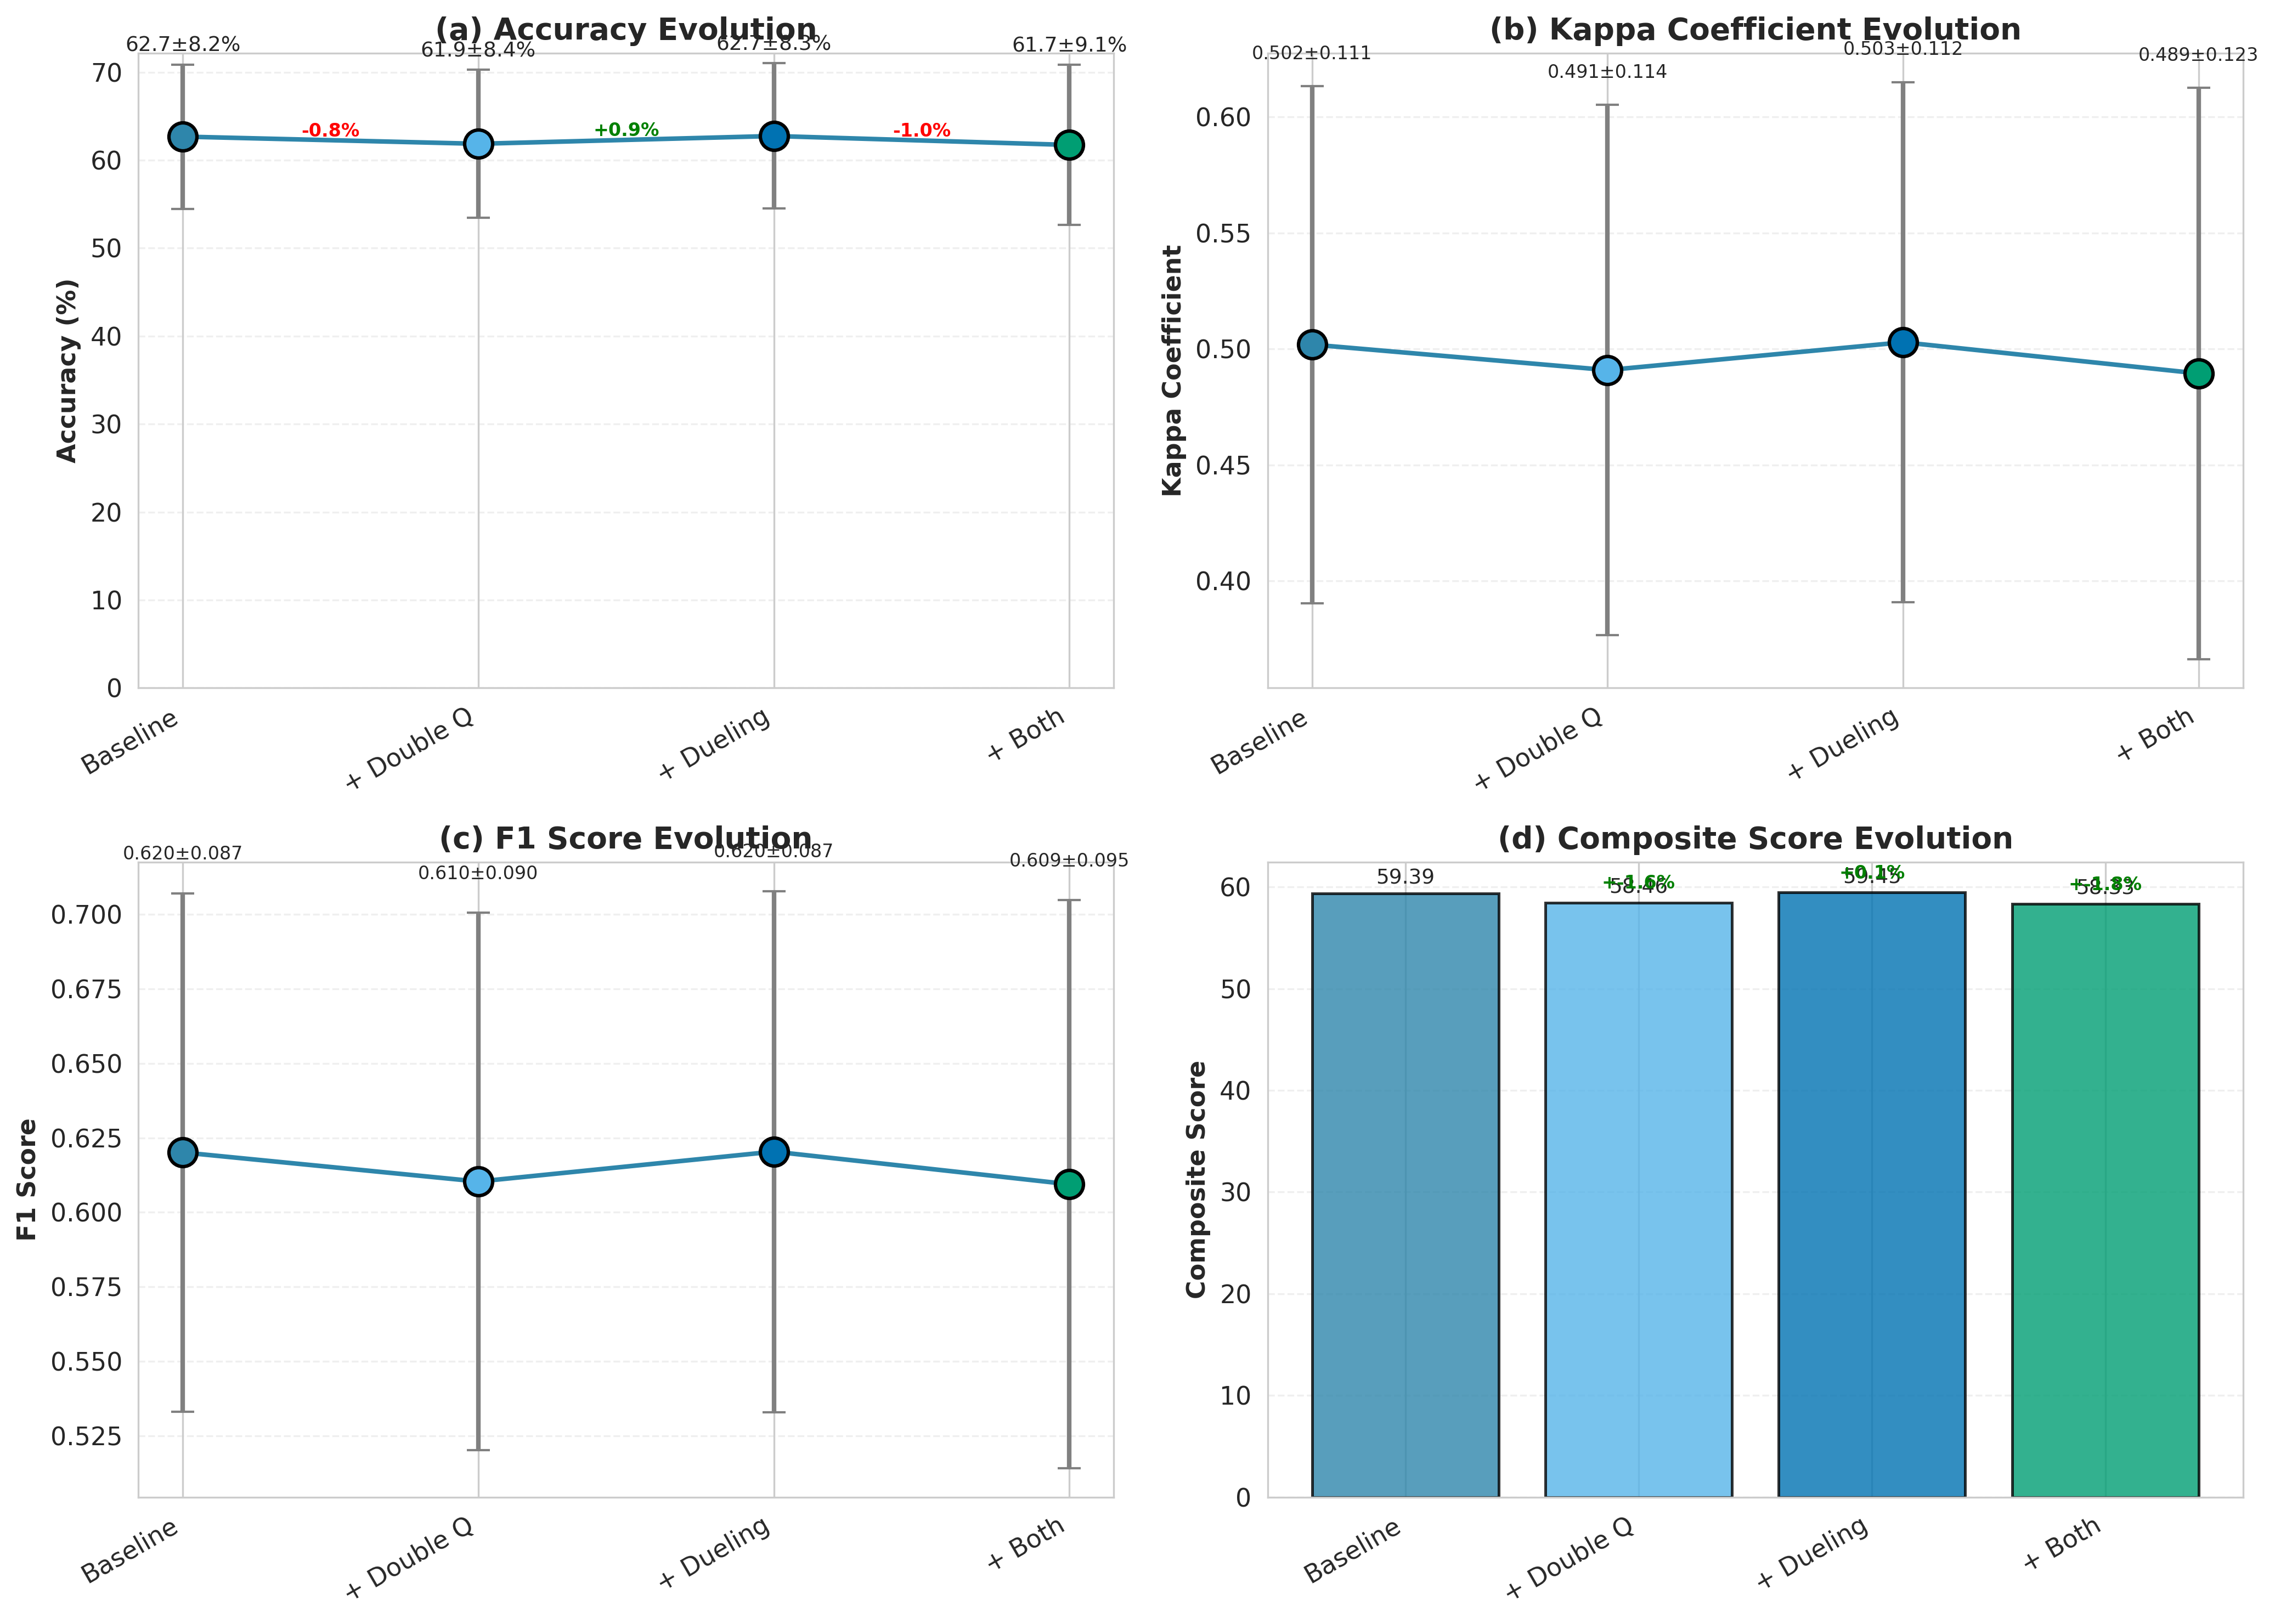
\includegraphics[width=0.85\textwidth]{figures/ablation/04_performance_evolution.png}
    \end{center}
\end{frame}

\begin{frame}{Q-Learning 改进策略消融实验分析}
    \begin{alertblock}{性能演变}
        \footnotesize
        \begin{itemize}
            \item \textbf{Baseline}：62.7\% 准确率
            \item \textbf{+ Double Q}：下降至 61.9\% (-0.8\%)
            \item \textbf{+ Dueling}：恢复至 62.7\% (+0.9\%)
            \item \textbf{+ Both}：略降至 61.7\% (-1.0\%)
            \item \textbf{结论}：Dueling 架构维持性能，Double Q 未带来预期收益
        \end{itemize}
    \end{alertblock}

    \vspace{0.2cm}
    \begin{exampleblock}{结果分析}
        \footnotesize
        Baseline 准确率为 62.7\%，引入 Double Q 后略微下降至 61.9\% (-0.8\%)，引入 Dueling 架构后恢复至 62.7\% (+0.9\%)，而两者结合（Dueling Double Q-Learning）略降至 61.7\% (-1.0\%)。Kappa 系数和 F1 分数趋势与准确率一致，Baseline (0.502) 与 + Dueling (0.503) 表现最佳，涉及 Double Q 的变体略低（0.491 和 0.489）。结果表明，在本任务中，\textbf{Dueling 架构能维持基线性能，但 Double Q 机制并未带来预期收益}，Standard Q-Learning 已是最优选择。
    \end{exampleblock}
\end{frame}

\begin{frame}{时间窗口选择演变分析}
    \begin{center}
    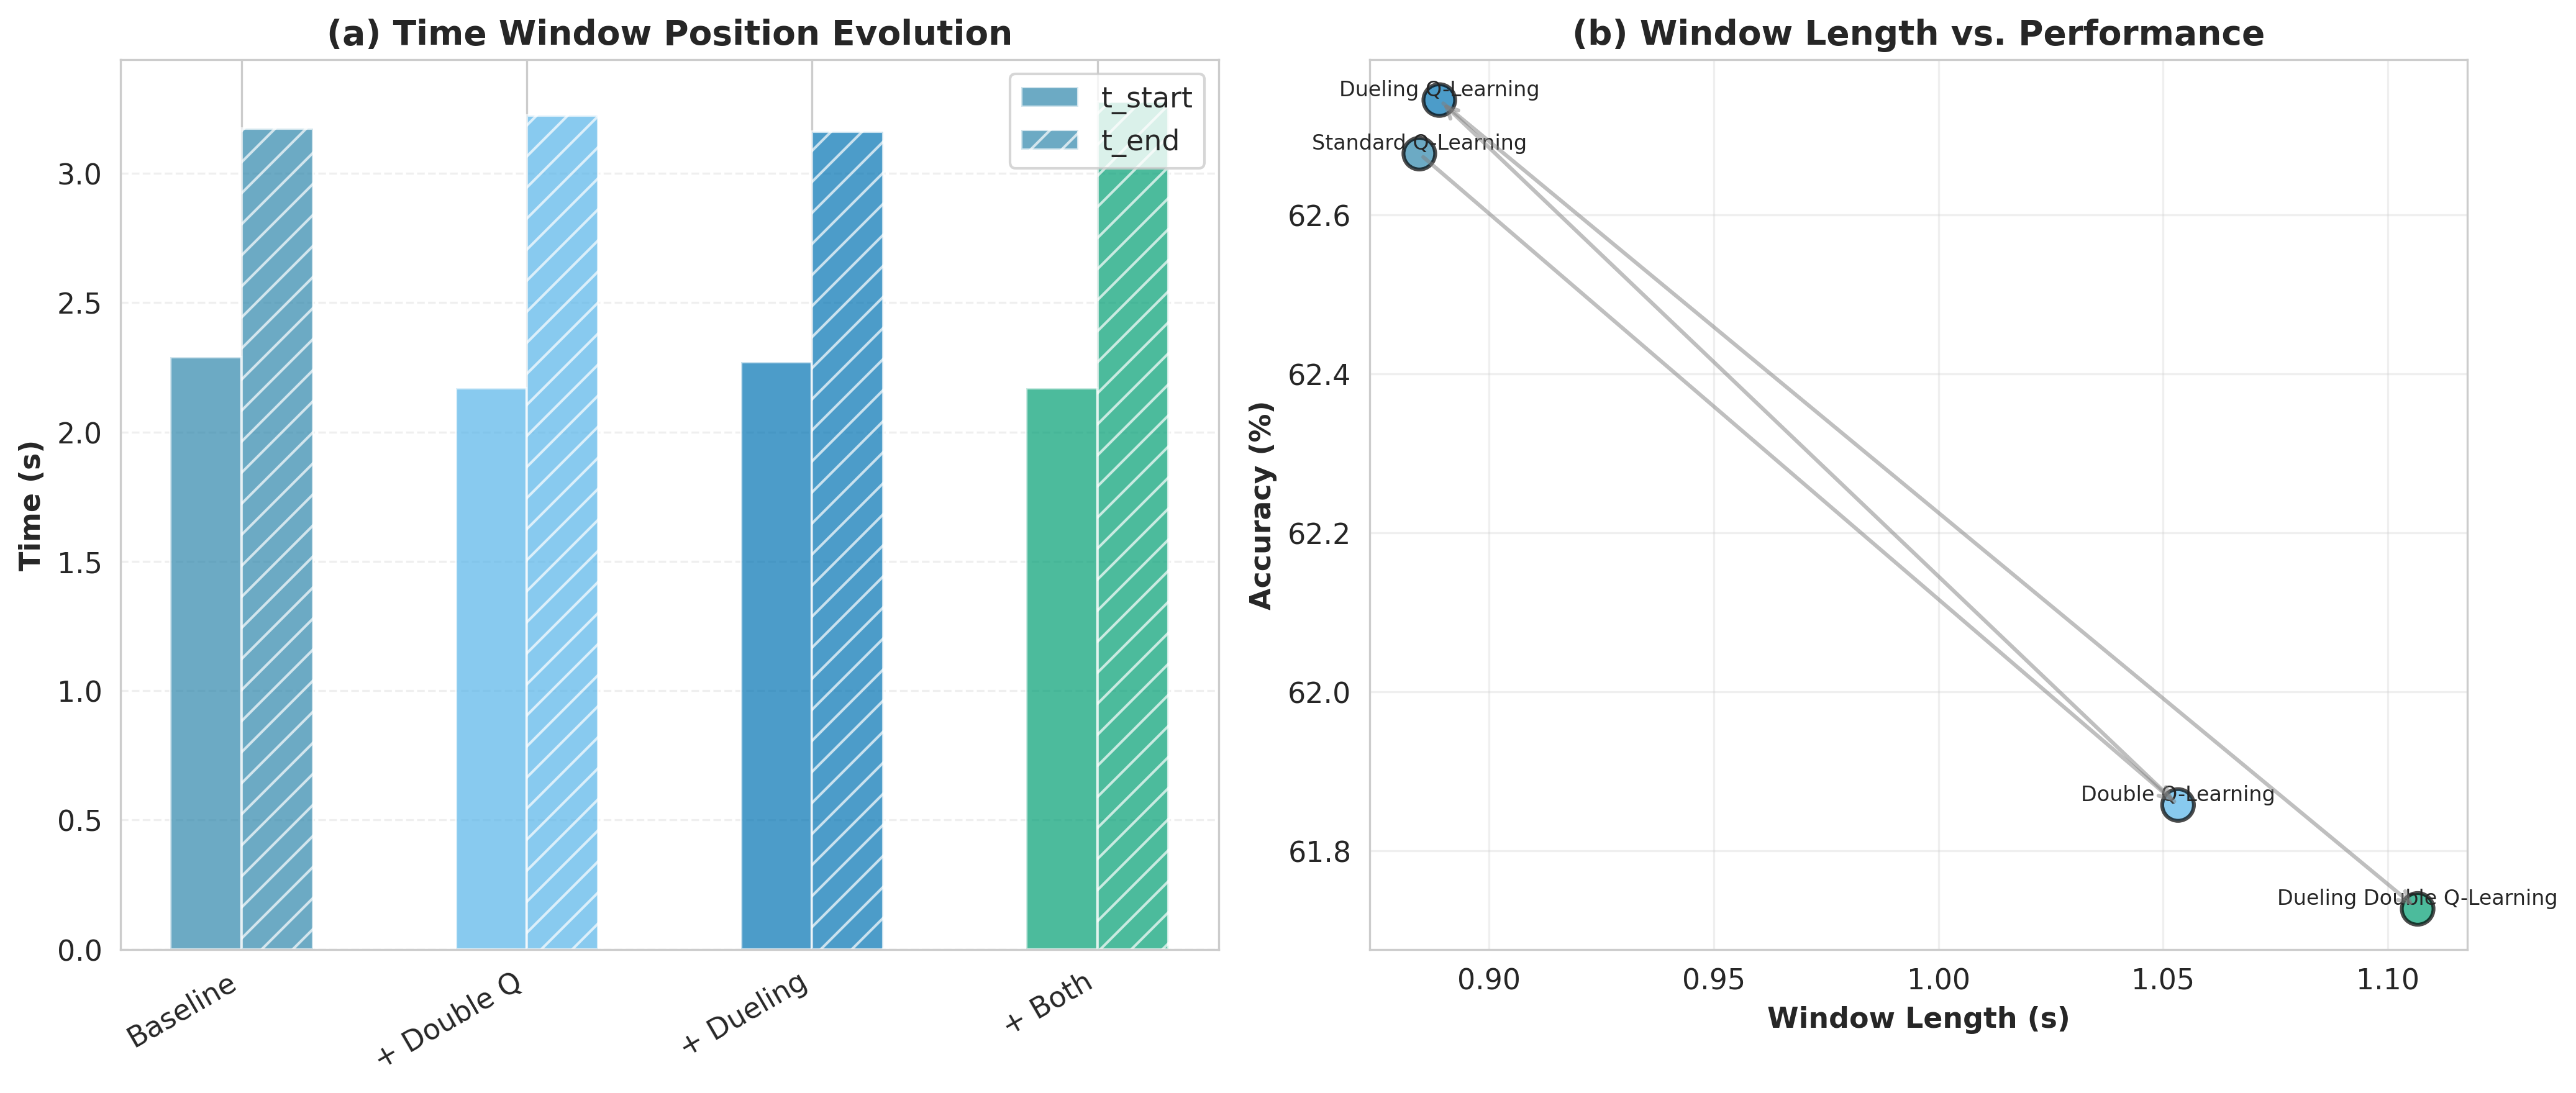
\includegraphics[width=0.85\textwidth]{figures/ablation/04_window_evolution.png}
    \end{center}
\end{frame}

\begin{frame}{时间窗口选择演变分析}
    \begin{exampleblock}{窗口模式}
        \footnotesize
        \begin{itemize}
            \item \textbf{位置}：所有方法一致选择后期片段 (起始约 2.2s，结束约 3.3s)
            \item \textbf{窗口长度与性能}：显著负相关
            \item \textbf{Standard/Dueling Q}：短窗口 (0.9s)，高准确率 (62.7\%)
            \item \textbf{Double Q 变体}：长窗口 (1.05s--1.1s)，略低准确率 (61.7\%--61.9\%)
            \item \textbf{结论}：精简窗口 (0.9s) 更利于捕捉判别性特征
        \end{itemize}
    \end{exampleblock}

    \vspace{0.2cm}
    \begin{alertblock}{结果分析}
        \footnotesize
        所有方法均一致地选择试验后期的时间片段（起始约 2.2s，结束约 3.2s--3.3s），验证了运动想象关键特征分布的时间稳定性。窗口长度与分类准确率的关系散点图显示显著的负相关趋势：Standard Q-Learning 和 Dueling Q-Learning 选择了较短的窗口（约 0.9s），取得了更高的准确率（62.7\%）；而引入 Double Q 机制的变体倾向于选择较长的窗口（1.05s--1.1s），准确率略低（61.7\%--61.9\%）。这表明\textbf{精简的时间窗口（约 0.9s）更有利于捕捉判别性特征并抑制噪声干扰}。
    \end{alertblock}
\end{frame}

\begin{frame}{改进策略详细分析}
    \begin{center}
    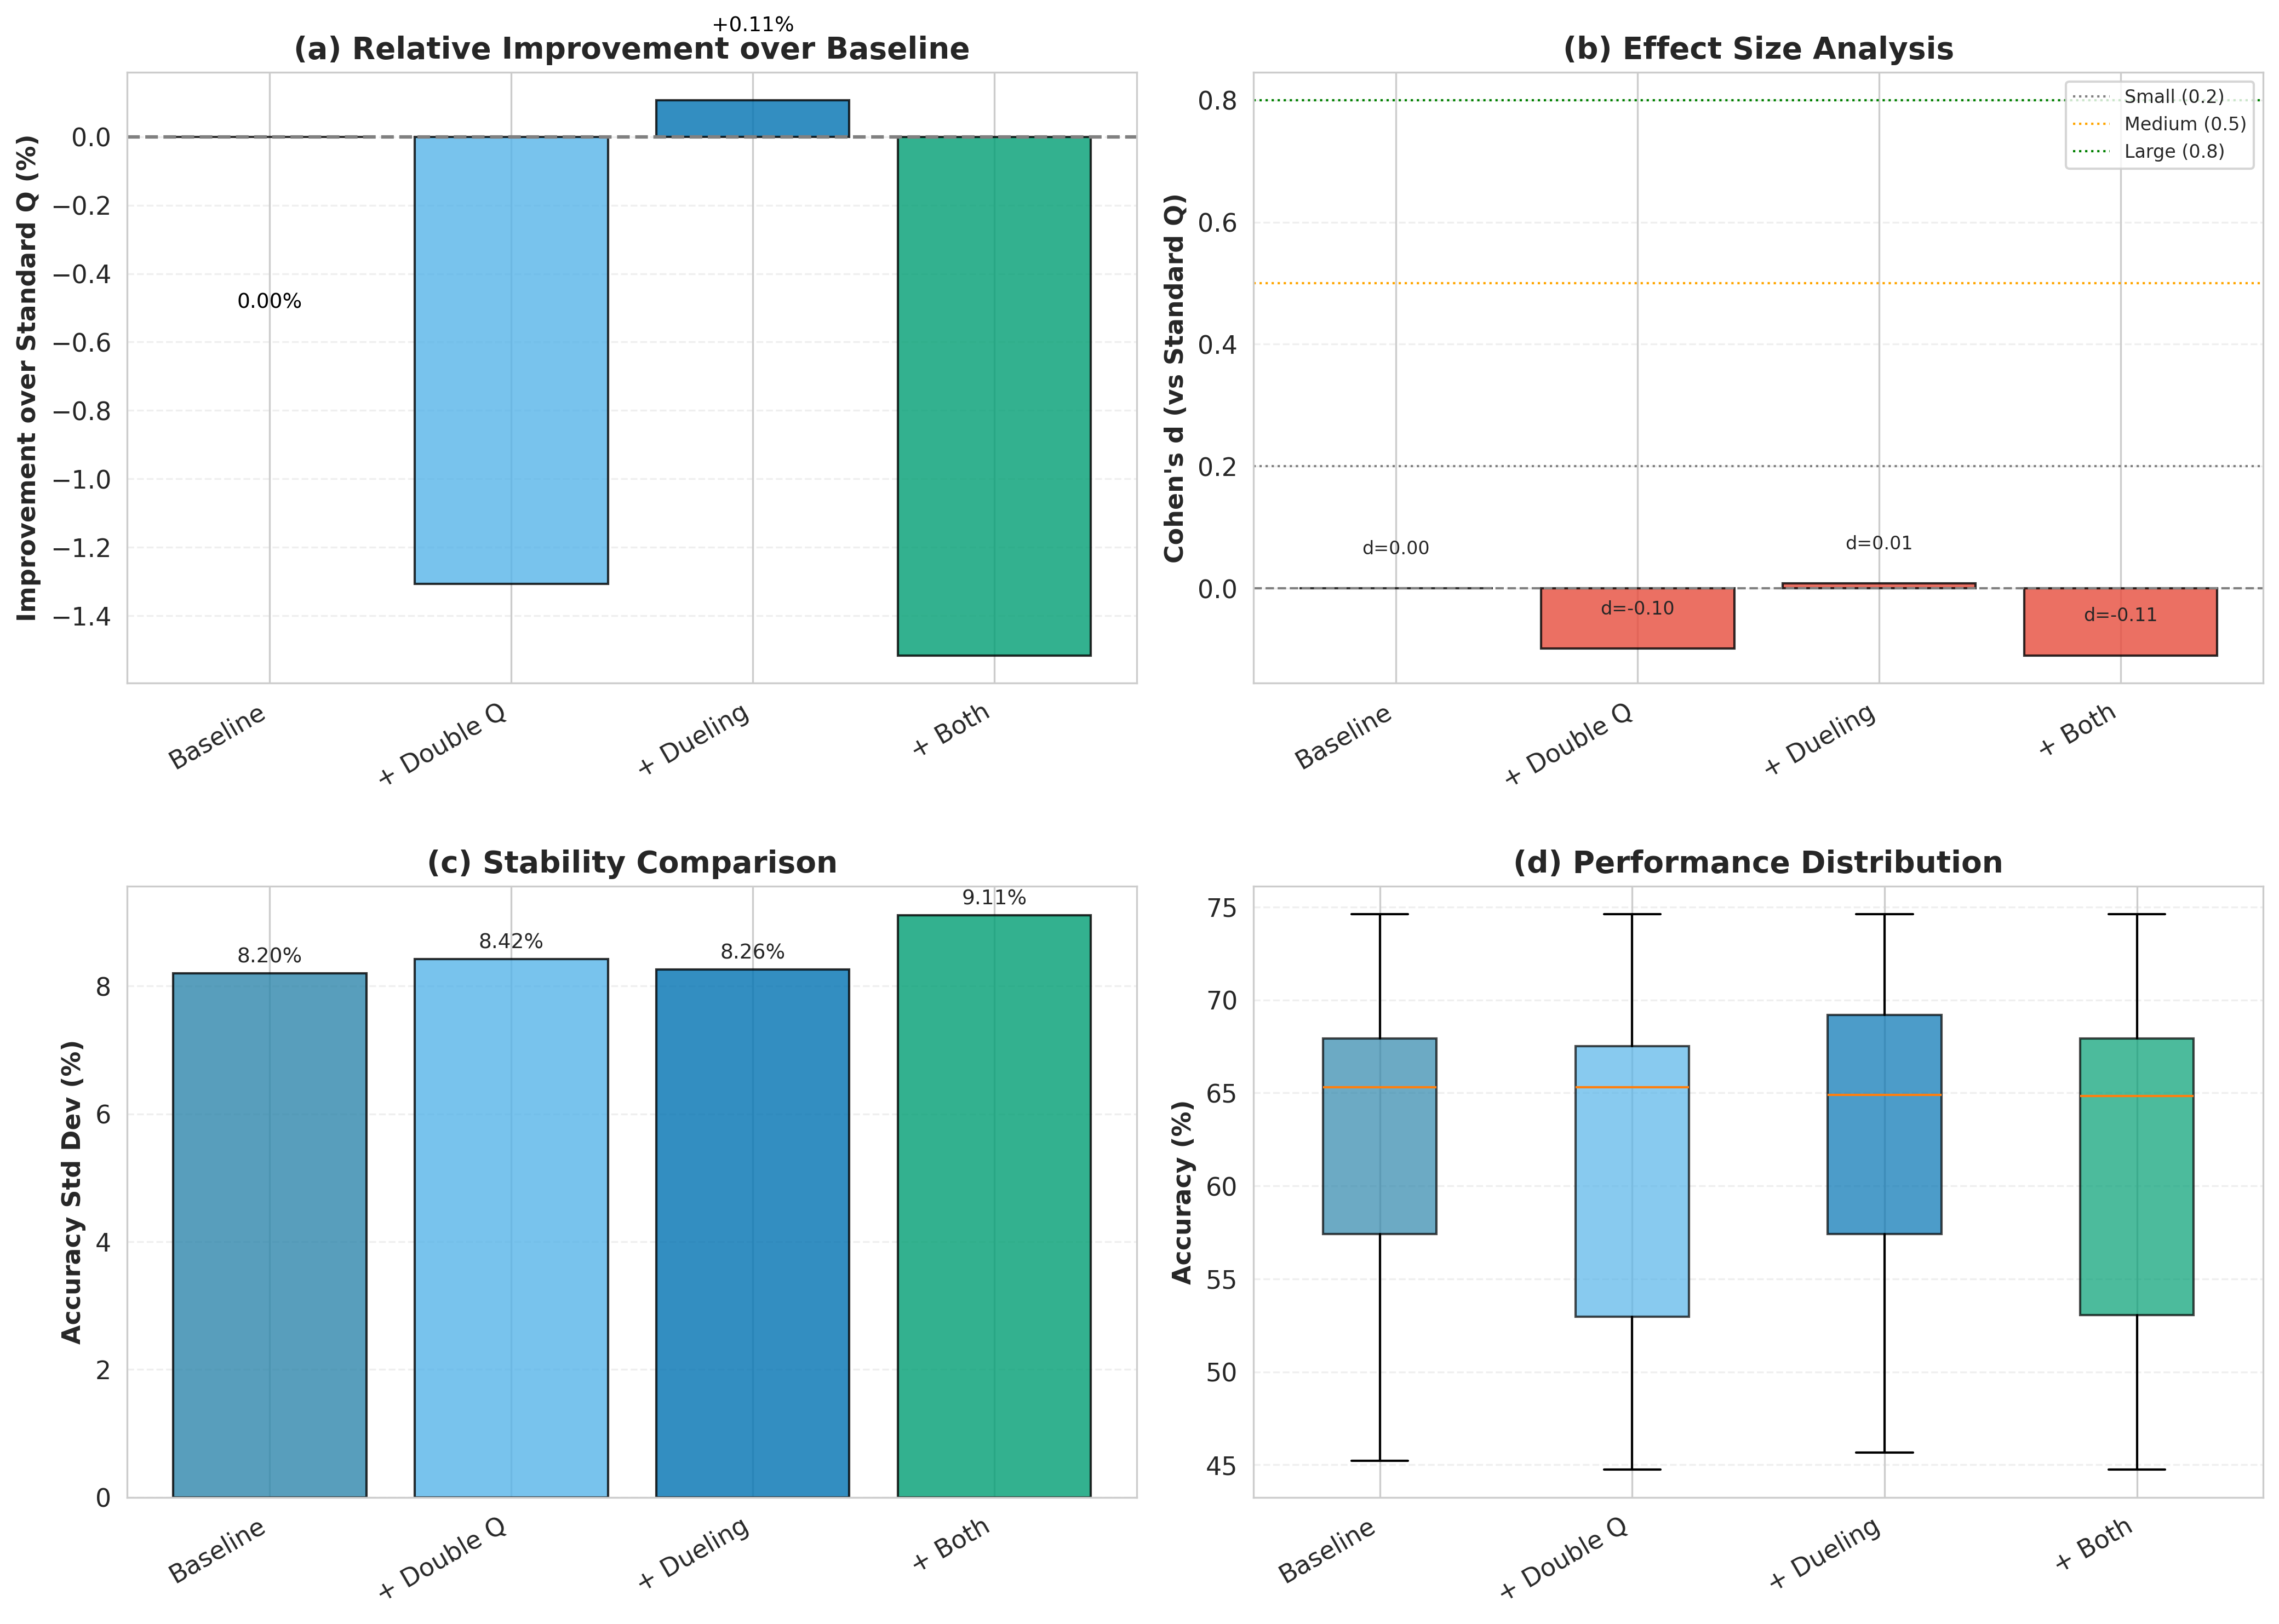
\includegraphics[width=0.85\textwidth]{figures/ablation/04_improvement_analysis.png}
    \end{center}
\end{frame}

\begin{frame}{改进策略详细分析}
    \begin{alertblock}{综合分析}
        \footnotesize
        \begin{itemize}
            \item \textbf{相对提升}：Dueling (+0.11\%)，Double Q (-1.3\%)，Both (-1.5\%)
            \item \textbf{效应量}：所有$|d| < 0.2$，Double Q 和 Both 显示微小负效应
            \item \textbf{稳定性}：Baseline 最优 (8.20\%)，Both 波动最大 (9.11\%)
            \item \textbf{结论}：Standard Q-Learning 已是最优选择，复杂机制增加开销
        \end{itemize}
    \end{alertblock}

    \vspace{0.2cm}
    \begin{exampleblock}{结果分析}
        \footnotesize
        Dueling 架构带来了微小的正向提升（+0.11\%），而引入 Double Q 机制（-1.3\%）及两者结合（Both, -1.5\%）均导致性能下降。所有变体与基线的效应量均远小于小效应阈值（$|d| < 0.2$）。Baseline 表现出最佳的稳定性（Std Dev = 8.20\%），而 + Both 的波动性最大（9.11\%）。综合分析表明，\textbf{Standard Q-Learning 已足以有效解决本任务的时间窗口选择问题}，引入 Double Q 或 Dueling 等复杂机制不仅未能提升性能，反而可能增加计算复杂度并略微降低稳定性。
    \end{exampleblock}
\end{frame}

\begin{frame}{消融实验详细对比}
    \begin{center}
    \footnotesize
    \renewcommand{\arraystretch}{1.3}
    \begin{tabular}{lcccc}
        \hline
        \textbf{Method} & \textbf{Accuracy (\%)} & \textbf{Kappa} & \textbf{F1} & \textbf{Std Dev (\%)} \\
        \hline
        Baseline (Standard Q) & \textbf{62.68 $\pm$ 8.20} & 0.502 & 0.620 & \textbf{8.20} \\
        + Double Q & 61.86 $\pm$ 8.42 & 0.491 & 0.610 & 8.42 \\
        + Dueling & 62.74 $\pm$ 8.26 & 0.503 & 0.620 & 8.26 \\
        + Both & 61.73 $\pm$ 9.11 & 0.489 & 0.609 & 9.11 \\
        \hline
    \end{tabular}
    \end{center}
\end{frame}

\begin{frame}{消融实验结论}
    \begin{exampleblock}{消融结论}
        \footnotesize
        \begin{itemize}
            \item Standard Q-Learning 在准确率和稳定性上均表现最优
            \item Double Q 机制导致性能下降 (-0.82\%) 和稳定性降低
            \item Dueling 架构维持基线性能，但无显著提升
            \item \textbf{最终选择}：Standard Q-Learning 为本任务最优方案
        \end{itemize}
    \end{exampleblock}
\end{frame}

% ============================================================================
% 本章小结
% ============================================================================
\subsection{本章小结}

\begin{frame}{本章小结}
    \begin{alertblock}{实验结论}
        \footnotesize
        \begin{itemize}
            \item \textbf{基线对比}：搜索优化方法 (63.3\%) 显著优于固定窗口 (45\%)
            \item \textbf{Q-Learning vs 基线}：性能相当 (62.7\% vs 63.3\%)，差异不显著
            \item \textbf{Table Q-Learning vs DQN}：准确率差异仅 -0.02\% ($p=0.981$)
            \item \textbf{消融实验}：Standard Q-Learning 为最优选择
        \end{itemize}
    \end{alertblock}

    \vspace{0.2cm}
    \begin{exampleblock}{核心验证}
        \footnotesize
        \begin{itemize}
            \item 表格型 Q-Learning 可在不显著牺牲性能前提下替代 DQN
            \item 稳定性优于 DQN (标准差降低 10.97\%)
            \item 推理效率$O(1)$查表，满足实时 BCI 要求
        \end{itemize}
    \end{exampleblock}
\end{frame}

} % end of \small
     % 实验与结果分析
% ============================================================================
% 第五章：总结与展望
% 优化说明：精简结构，内容深入，避免复杂嵌套
% ============================================================================

\section{总结与展望}

{\footnotesize

% ============================================================================
% 研究总结
% ============================================================================
\subsection{研究总结}

\begin{frame}{研究背景与核心问题}
    \begin{block}{MI-BCI 应用前景}
        \begin{itemize}
            \item \textbf{康复医疗}：脑卒中、脊髓损伤患者重建运动功能
            \item \textbf{人机交互}：为严重运动障碍患者提供新型控制方式
            \item \textbf{神经工程}：深化对大脑运动皮层 ERD/S 现象的理解
        \end{itemize}
    \end{block}

    \begin{block}{关键挑战：时间窗选择}
        \begin{itemize}
            \item \textbf{ERD 动态特性}：事件相关去同步化存在显著个体间差异（潜伏期 0.5--2s）
            \item \textbf{EEG 信号特性}：非平稳、低信噪比（SNR 约 $-10$ 至 $-20$ dB）
            \item \textbf{实时性要求}：在线 BCI 系统需毫秒级响应（延迟 $< 100$ms）
            \item \textbf{资源约束}：嵌入式设备内存通常 $< 1$MB，功耗 $< 100$mW
        \end{itemize}
    \end{block}

    \begin{block}{核心研究问题}
        如何在保持分类性能的前提下，实现轻量化、可解释、自适应的时间窗优化？
    \end{block}
\end{frame}

\begin{frame}{现有方法局限性分析}
    \begin{table}[h]
        \centering
        \renewcommand{\arraystretch}{1.3}
        \begin{tabular}{l|l|l}
            \hline
            \textbf{方法} & \textbf{局限性} & \textbf{复杂度} \\
            \hline
            固定时间窗 & 无法适应个体间差异 & $O(1)$ \\
            滑动窗 & 计算复杂度线性增长 & $O(n)$ \\
            贝叶斯优化 & 高维参数空间效率低 & $O(n^3)$ \\
            深度强化学习 & 百万参数、训练不稳定、黑盒决策 & $O(|\theta|)$ \\
            \hline
        \end{tabular}
    \end{table}

    \vspace{0.3cm}
    \begin{block}{核心矛盾}
        \begin{itemize}
            \item \textbf{DQN 的需求}：百万级参数、大量训练数据（$>10^5$ 样本）、GPU 加速
            \item \textbf{BCI 的现实}：数据稀缺（典型实验 $<1000$ 试次）、设备资源受限
            \item \textbf{根本问题}：模型复杂度与任务难度不匹配
        \end{itemize}
    \end{block}
\end{frame}

\begin{frame}{研究方法：表格型 Q-Learning}
    \begin{block}{马尔可夫决策过程形式化}
        \begin{itemize}
            \item \textbf{状态空间} $\mathcal{S}$：136 个离散时间窗状态（起始点 0--0.8s，终点 0.8--3.0s，步长 0.2s）
            \item \textbf{动作空间} $\mathcal{A}$：4 个边界调整动作 $\{t_s^-, t_s^+, t_e^-, t_e^+\}$
            \item \textbf{奖励函数} $R(s,a)$：CSP-SVM 5 折交叉验证准确率
            \item \textbf{状态转移} $P(s'|s,a)$：确定性过程
            \item \textbf{折扣因子} $\gamma = 0.95$：平衡即时与长期奖励
        \end{itemize}
    \end{block}

    \begin{block}{算法设计}
        \begin{itemize}
            \item \textbf{表格型表示}：维护 $Q(s,a)$ 表，参数数量 $=|\mathcal{S}|\times|\mathcal{A}|=544$
            \item \textbf{更新规则}：$Q(s,a) \leftarrow Q(s,a) + \alpha[r + \gamma\max_{a'}Q(s',a') - Q(s,a)]$
        \end{itemize}
    \end{block}

    \begin{block}{核心优势}
        轻量化（2KB 内存）$\cdot$ 收敛性保证（Watkins, 1989）$\cdot$ 可解释性强
    \end{block}
\end{frame}

\begin{frame}{实验结果与性能对比}
    \begin{center}
    \renewcommand{\arraystretch}{1.4}
    \begin{tabular}{lcc}
        \hline
        \textbf{指标} & \textbf{Table Q} & \textbf{DQN} \\
        \hline
        平均准确率 & 62.68\% & 62.70\% \\
        标准差 & $\pm 8.12\%$ & $\pm 8.05\%$ \\
        统计检验 & \multicolumn{2}{c}{$t(8) = 0.024, p = 0.981$} \\
        效应量 (Cohen's $d$) & \multicolumn{2}{c}{$0.003$（可忽略）} \\
        \hline

    \end{tabular}
    \end{center}

    \begin{block}{核心结论}
        \begin{itemize}
            \item 表格型 Q-Learning 在保持与 DQN 相当性能的同时，显著降低计算资源需求
            \item 性能差异无统计学意义 ($p > 0.05$)，效应量接近零
        \end{itemize}
    \end{block}
\end{frame}

\begin{frame}{计算效率详细对比}
    \begin{table}[h]
        \centering
        \renewcommand{\arraystretch}{1.3}
        \begin{tabular}{lccc}
            \hline
            \textbf{指标} & \textbf{Table Q} & \textbf{DQN} & \textbf{提升倍数} \\
            \hline
            参数量 & 544 & 1,211,776 & 2227$\times$ \\
            内存占用 & 2 KB & 250 KB & 125$\times$ \\
            推理延迟 & 0.001 ms & 1.2 ms & 1200$\times$ \\
            训练时间/被试 & 2.5 min & 7.8 min & 3.1$\times$ \\
            FLOPs/推理 & $\sim 10^2$ & $\sim 10^6$ & 10000$\times$ \\
            \hline
        \end{tabular}
    \end{table}
    
    \vspace{0.3cm}
    \begin{block}{嵌入式部署意义}
        \begin{itemize}
            \item Table Q 可在 ARM Cortex-M4（主频 80MHz, SRAM 320KB）上实时运行
            \item DQN 需高性能处理器（如 Cortex-A7）或专用 AI 加速器
            \item 功耗对比：Table Q $< 10$mW vs DQN $> 500$mW
        \end{itemize}
    \end{block}
\end{frame}

\begin{frame}{主要理论贡献}
    \begin{block}{轻量化 BCI 设计新范式}
        \begin{itemize}
            \item \textbf{核心思想}：将深度强化学习简化为表格型强化学习
            \item \textbf{设计原则}：模型复杂度与任务难度匹配，避免过度参数化
            \item \textbf{实现效果}：轻量化与高性能的统一，参数量减少 2227 倍
            \item \textbf{推广价值}：适用于其他状态空间有限的 BCI 优化任务
        \end{itemize}
    \end{block}

    \vspace{0.3cm}
    \begin{block}{算法选择准则}
        \begin{itemize}
            \item \textbf{适用边界}：状态空间 $|\mathcal{S}| < 10^4$ 且状态 - 动作对可充分访问
            \item \textbf{表格型优势}：收敛性保证、样本效率高、可解释性强、无超参数调优
            \item \textbf{DQN 适用场景}：$|\mathcal{S}| > 10^6$ 或连续状态空间
        \end{itemize}
    \end{block}
\end{frame}

\begin{frame}{主要实践贡献}
    \begin{block}{可解释性 BCI 系统实践}
        \begin{itemize}
            \item \textbf{Q 值表可视化}：可直接展示每个状态的最优动作和预期回报
            \item \textbf{学习轨迹追踪}：记录 Q 值收敛过程，分析智能体学习动态
            \item \textbf{决策透明度}：医生/研究者可以理解系统为何选择特定时间窗
            \item \textbf{临床转化价值}：可解释性是医疗 AI 系统审批的关键前提
        \end{itemize}
    \end{block}

    \vspace{0.3cm}
    \begin{block}{实验验证体系}
        \begin{itemize}
            \item \textbf{对比方法}：10 种系统性评估（固定窗、DQN、4 种 Q-Learning 变体等）
            \item \textbf{统计检验}：配对样本 $t$ 检验 + 效应量分析 (Cohen's $d$)
            \item \textbf{被试分析}：9 名被试个体级别性能详细对比
            \item \textbf{消融实验}：验证各算法组件的贡献
        \end{itemize}
    \end{block}
\end{frame}

% ============================================================================
% 研究局限性
% ============================================================================
\subsection{研究局限性}

\begin{frame}{研究局限性 1/3}
    \begin{block}{验证范围的局限}
        \begin{itemize}
            \item \textbf{数据集单一}：仅 BCI Competition IV 2a，缺乏跨数据集验证
            \item \textbf{被试群体局限}：9 名健康被试，未包含脑卒中患者
            \begin{itemize}
                \item 患者脑电信号非平稳性更强、信噪比更低
                \item 可能存在病灶侧运动皮层功能重组
            \end{itemize}
            \item \textbf{验证场景}：离线分析，未在线闭环验证
            \item \textbf{统计效力}：样本量 $N=9$，统计检验效力约 0.6
        \end{itemize}
    \end{block}

    \vspace{0.3cm}
    \begin{block}{方法设计的局限}
        \begin{itemize}
            \item \textbf{离散化步长}：0.2 秒，可能无法定位全局最优的连续时间点
            \item \textbf{间接奖励}：通过 CSP-SVM 准确率间接构建，非直接衡量时间窗质量
            \item \textbf{干扰因素}：分类准确率受 CSP 特征质量、SVM 参数等影响
            \item \textbf{潜在改进}：探索 ERD 强度、信噪比、互信息等直接奖励信号
        \end{itemize}
    \end{block}
\end{frame}

\begin{frame}{研究局限性 2/3}
    \begin{block}{Q-Learning 变体研究不足}
        \begin{itemize}
            \item \textbf{已对比变体}：Standard、Double、Dueling、Dueling Double Q-Learning
            \item \textbf{现象观察}：Double Q-Learning 性能略低于 Standard Q-Learning
            \item \textbf{机制分析不足}：
            \begin{itemize}
                \item 双 Q 网络的过估计修正在本任务中可能过于保守
                \item 状态空间有限、奖励确定性高时，Standard Q-Learning 过估计问题不显著
            \end{itemize}
            \item \textbf{未探索变体}：Prioritized Experience Replay、Noisy Nets、Distributional RL
            \item \textbf{Q 值表演化分析缺失}：未分析收敛速度、Q 值分布时空模式
        \end{itemize}
    \end{block}
\end{frame}

\begin{frame}{研究局限性 3/3}
    \begin{block}{通用性的局限}
        \begin{itemize}
            \item \textbf{分类器依赖}：仅 CSP-SVM，未验证 EEGNet、Shallow FBCSP 等深度学习模型
            \item \textbf{BCI 范式单一}：仅运动想象，未验证 SSVEP、P300 等范式
            \item \textbf{嵌入式测试缺乏}：未在 ARM Cortex-M 系列单片机上部署验证
        \end{itemize}
    \end{block}

    \vspace{0.3cm}
    \begin{block}{分析维度的局限}
        \begin{itemize}
            \item \textbf{理论分析为主}：参数计数、FLOPs、复杂度分析
            \item \textbf{缺乏实证基准}：未测量实际运行时间、功耗、温度影响
        \end{itemize}
    \end{block}
\end{frame}

% ============================================================================
% 未来工作展望
% ============================================================================
\subsection{未来工作展望}

\begin{frame}{未来工作 1/3：在线和临床验证}
    \begin{block}{在线实时验证}
        \begin{itemize}
            \item \textbf{系统移植}：将 Q 表移植到 ARM Cortex-M4/M7 嵌入式系统
            \item \textbf{评估指标}：
                \item 端到端延迟：从 EEG 采集到反馈呈现（目标 $< 100$ms）
                \item 在线准确率：实时反馈场景下的分类性能
                \item 信息传输率 (ITR)：bits/min，综合评估系统性能
                \item 用户体验：NASA-TLX 认知负荷量表、系统可用性量表 (SUS)
        \end{itemize}
    \end{block}

    \begin{block}{临床验证}
        \begin{itemize}
            \item \textbf{目标群体}：脑卒中后运动功能障碍患者、脊髓损伤患者
            \item \textbf{试验设计}：样本量 $N \geq 30$，4--8 周干预，每周 3--5 次训练
            \item \textbf{评估工具}：Fugl-Meyer 运动功能评分、Barthel 指数
            \item \textbf{预期价值}：为实际应用价值提供循证医学证据
        \end{itemize}
    \end{block}
\end{frame}

\begin{frame}{未来工作 2/3：算法效率优化}
    \begin{block}{快速奖励估计方法}
        \begin{itemize}
            \item \textbf{基于元学习}：学习奖励函数的代理模型，新被试只需少量试次
            \item \textbf{缓存机制}：复用历史被试交叉验证结果，基于相似度检索
            \item \textbf{目标}：离线训练时间从分钟级缩短到秒级，实现"即插即用"
        \end{itemize}
    \end{block}

    \begin{block}{时间窗精度提升}
        \begin{itemize}
            \item \textbf{更精细离散化}：探索 0.1 秒步长(状态数增至约 500，仍远小于 DQN)
            \item \textbf{混合优化策略}：第一阶段：表格型 Q-Learning 粗搜索；第二阶段：贝叶斯优化/梯度方法精搜索
            \item \textbf{连续时间建模}：探索连续时间强化学习方法
        \end{itemize}
    \end{block}
\end{frame}

\begin{frame}{未来工作 3/3：泛化与迁移}
    \begin{block}{算法泛化能力}
        \begin{itemize}
            \item \textbf{深度学习结合}：与 EEGNet、Shallow FBCSP 等模型结合
            \item \textbf{空间层面优化}：
            \begin{itemize}
                \item 通道选择：基于强化学习选择最优 EEG 通道子集
                \item CSP 空间滤波器优化：联合优化分量数和参数
                \item 时空联合优化：统一建模为 MDP，实现时空特征协同优化
            \end{itemize}
        \end{itemize}
    \end{block}

    \vspace{0.3cm}
    \begin{block}{迁移学习策略}
        \begin{itemize}
            \item \textbf{核心思路}：从不同被试的最优 Q 表中提取通用先验知识
            \item \textbf{技术路线}：聚类分析 $\rightarrow$ 原型提取 $\rightarrow$ 快速适配
            \item \textbf{预期收益}：校准时间从 30 分钟缩短至 5 分钟，降低使用门槛
        \end{itemize}
    \end{block}
\end{frame}

% ============================================================================
% 本章小结
% ============================================================================
\subsection{本章小结}

\begin{frame}{本章小结}
    \begin{block}{研究总结}
        \begin{itemize}
            \item \textbf{核心方法}：提出表格型 Q-Learning 轻量化时间窗优化方法
            \item \textbf{性能表现}：与 DQN 无显著差异 ($t(8)=0.024, p=0.981, d=0.003$)
            \item \textbf{四大贡献}：
            \begin{itemize}
                \item 轻量化 BCI 设计新范式
                \item 算法选择准则（$|\mathcal{S}| < 10^4$ 时表格型优于 DQN）
                \item 可解释性 BCI 系统实践
                \item 完善的实验验证体系
            \end{itemize}
        \end{itemize}
    \end{block}

    \begin{block}{研究局限性}
        验证范围~$\cdot$ 方法设计~$\cdot$ 变体研究~$\cdot$ 通用性~$\cdot$ 分析维度
    \end{block}

    \begin{block}{未来方向}
        在线临床验证~$\cdot$ 算法效率优化~$\cdot$ 泛化能力探索~$\cdot$ 迁移学习
    \end{block}
\end{frame}

\begin{frame}{研究的理论意义与实践价值}
    \begin{block}{理论意义}
        \begin{itemize}
            \item \textbf{强化学习在 BCI 中的应用边界}：明确表格型与深度强化学习的适用场景
            \item \textbf{轻量化 AI 设计原则}：为资源受限场景下的模型选择提供理论指导
            \item \textbf{可解释性 BCI 方法论}：提供可解释性系统设计的实践参考
        \end{itemize}
    \end{block}

    \begin{block}{实践价值}
        \begin{itemize}
            \item \textbf{便携式 BCI 设备}：使高性能时间窗优化可在嵌入式设备部署
            \item \textbf{康复医疗应用}：为脑卒中患者提供可负担的 BCI 康复方案
            \item \textbf{技术转化潜力}：低功耗、低成本、可解释性支撑临床审批
        \end{itemize}
    \end{block}

    \begin{block}{结语}
        \centering
        \large
        轻量化设计~$\cdot$ 性能保证~$\cdot$ 可解释性~$\cdot$ 临床转化
    \end{block}
\end{frame}

} % end of \footnotesize
      % 总结与展望

% ---------- 附录：参考文献 ----------
\appendix

\begin{frame}[allowframebreaks]
    \frametitle{参考文献}
    \scriptsize
    \bibliography{slides}
\end{frame}

\end{document}
